\documentclass[a4paper,10pt]{book}
\usepackage[pdftex]{graphicx}
\usepackage{epstopdf}
\usepackage{subfigure}
\usepackage{amsmath,amsthm}
\usepackage{tikz}
\usepackage{circuitikz}
\usetikzlibrary{babel}
\usetikzlibrary{shapes, arrows, patterns, angles, quotes}
\textwidth= 15cm
\evensidemargin=0cm
\usepackage[spanish]{babel}
\usepackage[utf8]{inputenc}
\usepackage{textcomp}
\usepackage{amstext}
\usepackage{amsfonts}
\usepackage{amssymb}
\usepackage[hyperindex=true,breaklinks=true,colorlinks=true,linkcolor=blue]{hyperref}
\renewcommand{\tablename}{Tabla}
\renewcommand{\listtablename}{\'Indice de Tablas}

\usepackage{listings}
\usepackage{color} %red, green, blue, yellow, cyan, magenta, black, white
\definecolor{mygreen}{RGB}{28,172,0} % color values Red, Green, Blue
\definecolor{mylilas}{RGB}{170,55,241}

\usepackage{multirow}
\usepackage{makeidx}

%\usepackage{draftwatermark}
%\SetWatermarkText{Borrador,juan.jimenez@fis.ucm.es}
%\SetWatermarkScale{2}

% Atajos para el tikz
\tikzstyle{block} = [draw, rectangle, minimum width=6em]
\tikzstyle{sum} = [draw, fill=blue!20, circle, node distance=1cm]
\tikzstyle{input} = [coordinate]
\tikzstyle{output} = [coordinate]
\tikzstyle{pinstyle} = [pin edge={to-,thin,black}]

% Entornos para los "teoremas"
\newtheorem{algo}{Algoritmo}[section]
\newtheorem{theorem}{Teorema}[section]
\newtheorem{problem}{Problema}[section]
\newtheorem{corollary}{Corolario}[section]
\newtheorem{lemmas}{Lema}[section]
\newcommand*{\lema}{Lema}
\newenvironment{lemma}[1][\lema]{\begin{lemmas}[#1]\renewcommand*{\qedsymbol}{\(\Diamond\)}}{\end{lemmas}}

\theoremstyle{definition}
%\newtheorem{definition}{Definición}[section]
\newtheorem{definitions}{Definición}[section]
\newcommand*{\definicion}{Definición}
\newenvironment{definition}[1][\definicion]{\begin{definitions}[#1]\renewcommand*{\qedsymbol}{\(\bigtriangledown\)}}{\end{definitions}}

\newtheorem{examples}{Ejemplo}[section]
\newcommand*{\ejemplo}{Ejemplo}
\newenvironment{example}[1][\ejemplo]{\begin{examples}[#1]\renewcommand*{\qedsymbol}{\(\maltese\)}}{\end{examples}}
%\renewcommand{\qedsymbol}{\maltese}

\theoremstyle{remark}
\newtheorem{remark}{Atención}[section]

\graphicspath{{./figuras/}}
\makeindex
\begin{document}
\title{
\begin{flushleft}

\includegraphics[width=2.5cm]{ucm2.eps}
Universidad Complutense de Madrid\\
---------------------------------------------------------------------\
\end{flushleft}
Sistemas din\'amicos y realimentaci\'on}
\author{ Juan Jim\'enez \\ H\'ector Garc\'ia de Marina}

\maketitle\
\
\vspace*{\fill}

\includegraphics[scale=1]{by-sa.eps}\\
El contenido de estos apuntes est\'e1 bajo licencia Creative Commons Atribution-ShareAlike 4.0\\
\href{http://creativecommons.org/licenses/by-sa/4.0/}{http://creativecommons.org/licenses/by-sa/4.0/}\\
\copyright Juan Jim\'enez

\bigskip
\tableofcontents
\listoffigures
\listoftables
%\section*{Matlab Code}
\lstset{language=Matlab,%
    %basicstyle=\color{red},
    breaklines=true,%
    morekeywords={matlab2tikz},
    keywordstyle=\color{blue},%
    morekeywords=[2]{1}, keywordstyle=[2]{\color{black}},
    identifierstyle=\color{black},%
    stringstyle=\color{mylilas},
    commentstyle=\color{mygreen},%
    showstringspaces=false,%without this there will be a symbol in the places where there is a space
    numbers=left,%
    numberstyle={\tiny \color{black}},% size of the numbers
    numbersep=9pt, % this defines how far the numbers are from the text
    emph=[1]{for,end,break},emphstyle=[1]\color{red}, %some words to emphasise
    %emph=[2]{word1,word2}, emphstyle=[2]{style},    
}
\chapter{Introducción}
Estas notas de clase, conforman el contenido de la asignatura "Sistemas Dinámicos y Realimentación". La asignatura está especialmente orientada  a los estudiante del grado en Física y contiene tan solo dos ideas básicas:

\begin{enumerate}
\item Una parte apreciable --si no toda-- la realidad física que conocemos puede modelarse mediante el uso de lo que denominaremos sistemas dinámicos. Éstos vendrán caracterizados por un conjunto de variables de estado, que describen aspectos mensurables de la realidad y son dinámicos en el sentido de que el valor de las variables de estado evoluciona en el tiempo. Una manera habitual de describir un sistema dinámico, a partir de sus variables de estado, es mediante el uso de ecuaciones diferenciales\footnote{Para sistemas que evolucionan en tiempo continuo $t\in \mathbb{R}^+$. Para sistemas de tiempo discreto $t \in \mathbb{N}$ se emplean ecuaciones en diferencias. Por falta de tiempo, no estudiaremos sistemas de tiempo discreto en esta asignatura, aunque tienen un gran interés tanto en sí mismos como por su relación con los sistemas de tiempo continuo.}:

\begin{equation}
	\Sigma := \begin{cases}
		\dot x(t) =& f(t,x(t),u(t)) \\ y(t) =& g(t,x(t),u(t))
	\end{cases}, 
\label{eq: sigma}
\end{equation}
en donde $\dot x := \frac{\mathrm{d}}{\mathrm{dt}}(x(t))$ es la notación para la derivada total con respecto del tiempo, y $f:\mathbb{R} \times \mathbb{R}^n \times \mathbb{R}^k \to \mathbb{R}^n$ y $g: \mathbb{R} \times \mathbb{R}^n \times \mathbb{R}^k \to \mathbb{R}^m$ son funciones. Las variables de estado se agrupan en el vector $x(t)$.  El vector $u(t)$ agrupa las variables de entrada que representan magnitudes físicas externas al sistema cuyos valores influyen en la evolución de las variables de estado. Por último el vector $y(t)$ representa las salidas del sistema: magnitudes físicas, dependientes de las variables de estado y de las entradas, que pueden ser observadas (medidas). 

\item En muchos sistemas es posible manipular los valores de las variables de entrada de modo que se pueda obtener una evolución deseada de sus variables de estado y, por tanto, de su salida. El estudio de los modos de manipular las variables de entrada para conseguir la evolución deseada del sistema constituye lo que se conoce como \emph{Control de Sistemas}.

Una forma particularmente adecuada y poderosa, de manipular las variables de entrada para controlar la evolución de un sistema, es hacerlas depender de los valores que toman las variables de estado mismas: $u(t) = u(x(t))$ o de las salidas del sistema $u(t) = u(y(t))$. Esta manera de controlar un sistema se conoce como \emph{control por realimentación}.
\end{enumerate}

Podríamos decir que el estudio de los sistemas dinámicos tiene un carácter transversal ya que es aplicable a fenómenos físicos cualquier naturaleza; mecánicos, eléctricos, ópticos, etc. Además aplicando el conocido principio ''ecuaciones iguales tienen soluciones iguales'', podemos  con facilidad trasladar los resultados obtenidos en sistemas de una determinada naturaleza a otros distintos que puedan ser modelados con ecuaciones equivalentes. Así, por ejemplo, es posible establecer analogías entre sistemas mecánicos y sistemas eléctricos.

Un aspecto particularmente interesante en el estudio de los sistemas dinámicos, es el análisis de su estabilidad. En términos puramente intuitivos podríamos dar una definición preliminar de estabilidad diciendo que un sistema es estable cuando la evolución en el tiempo de sus variables de estado no diverge. A lo largo de la asignatura precisaremos este concepto, estudiaremos formas de establecer la estabilidad o no de un sistema y veremos su relación con la posibilidad de controlar un sistema mediante realimentación.

El concepto de realimentación está presente en la naturaleza. Los sistemas biológicos son capaces de reaccionar a su estado y modificarlo en beneficio propio.  Ejemplos de ello son la regulación del contenido de azúcar en sangre, de la temperatura corporal, o del equilibrio. En todos los casos, se parte del conocimiento del estado actual para actuar modificando el estado de modo que se alcance la situación deseada; a continuación, se vuelve a observar el estado resultante y se vuelve actuar, etc. Este ciclo observación-actuación-observación es un principio muy poderoso y está en la base del desarrollo científico y tecnológico. Los sistemas de control, basados en repetir dicho ciclo, son ubicuos. Están presentes en la industria, en los sistemas de comunicaciones, en el transporte y, por supuesto, en la investigación científica. Por ejemplo, el interferómetro de ondas gravitacionales  (LIGO) funciona gracias a un sofisticado sistema de control para estabilizarlo; el (gran) colisionador de hadrones (LHC) del CERN solo es una realidad gracias a los sistemas de control que permiten controlar los haces, mantener a baja temperatura sus electroimanes, etc.

La asignatura y el contenido de estos apuntes está divido en dos grandes bloques. Los temas 2, 3 y 4, son una introducción al estudio de los sistemas dinámicos no-lineales, su estabilidad y el diseño de algunos controladores básicos para este tipo de sistemas. Los capítulos 5 y 6 se centrar en el estudio de los sistemas lineales y su control por realimentación.  Se ha incluido también un apéndice con algunos ejemplos de uso de Matlab para resolver ejercicios de sistemas dinámicos.

Por último, los apuntes son para vosotros (los que estudiáis la asignatura). Están escritos en \LaTeX\ y todos los archivos fuente están colgados en el repositorio de GitHub \url{https://github.com/UCM-237/Realimentados}. Así que, si os animáis, podéis \emph{clonaros} el \emph{repo} y añadir cambiar y corregir todo lo que queráis a vuestros apuntes. Además, podéis enviarnos un \emph{pull request} cuando corrijáis errores, y así vamos mejorando los apuntes entre todos. Si no os va mucho git y/o \LaTeX\, también podéis enviar sugerencias y correcciones directamente al Campus Virtual o por correo electrónico.



\include{introduccion}
\chapter{Modelado de sistemas dinámicos}

\section{Sistemas en el espacio de estados}
Nos vamos a centrar en sistemas que puedan ser descritos por características cuantificables. A estas características las vamos a llamar {\bf estados}, como por ejemplo, una temperatura, una velocidad, o un voltaje. Si estos estados dependen del tiempo, entonces, llamamos {\bf señal} a la sucesión de valores de los estados en el tiempo. Uno podría interaccionar con el sistema a través de una {\bf entrada} cuantificable, y a su vez medir información del sistema a través de una {\bf salida} cuantificable.

Vamos a definir $x(t)\in\mathbb{R}^n$, $y(t)\in\mathbb{R}^m$ y $u(t)\in\mathbb{R}^k$ como el vector apilado de estados, la salida, y la entrada a un sistema $\Sigma$ respectivamente. En particular, son señales, e.g., $x :[0,\infty) \to \mathbb{R}^n$.

El sistema $\Sigma$ es un modelo que predice el valor de los estados y la salida a lo largo del tiempo. Esta predicción incorpora la interacción de la entrada con los estados y la salida. En particular, vamos a emplear ecuaciones diferenciales como herramienta para predecir la evolución en el tiempo de los estados del sistema $\Sigma$ como se muestra a continuación
\begin{equation}
	\Sigma := \begin{cases}
		\dot x(t) =& f(t,x(t),u(t)) \\ y(t) =& g(t,x(t),u(t))
	\end{cases}, 
\label{eq: sigma}
\end{equation}
en donde $\dot x := \frac{\mathrm{d}}{\mathrm{dt}}(x(t))$ es la notación para la derivada total con respecto del tiempo, y $f: \mathbb{R}^n \times \mathbb{R}^k \to \mathbb{R}^n$ y $g: \mathbb{R}^n \times \mathbb{R}^k \to \mathbb{R}^m$ son funciones.

Podemos representar el sistema $\Sigma$ como un bloque con puertos de entrada y de salida como se muestra en la figura \ref{fig: sigma}.

\begin{figure}[!h]
\centering
\begin{tikzpicture}[auto, node distance=2cm,>=latex']
	\node [input, name=input] {};
	\node [block, right of=input] (system) {$\Sigma$};
	\node [output, right of=system] (output) {};
	\draw [draw,->] (input) -- node {$u(t)$} (system);
	\draw [->] (system) -- node [name=y] {$y(t)$}(output);
\end{tikzpicture}
	\caption{Diagrama de bloque entrada/salida del sistema $\Sigma$.}
	\label{fig: sigma}
\end{figure}

Dado que el sistema viene descrito por las variables de estado,  con frecuencia es posible prescindir de la salida y centrar el estudio en la primera de las dos ecuaciones anteriores.

 En ocasiones podemos emplear para describir un sistema ecuaciones de estado en las que no aparece explícitamente la entrada,
\begin{equation}
\dot x = f(t,x)
\end{equation}\label{eq: for}
En este caso se, se habla de una ecuación de estado no forzada. Esto no quiere decir necesariamente que la entrada al sistema sea cero. Puede aparecer representada directamente como una función del tiempo, $u=\rho(t)$,  como una función (\emph{realimentación}) de los estados $u = \rho(x)$ o como una función de ambos $u=\rho(t,x)$.
Un caso especialmente interesante de (\ref{eq: for}) se obtiene cuando $f$ no depende explícitamente del tiempo,
\begin{equation}
\dot x = f(x)
\end{equation}
Se trata entonces de un sistema \emph{autónomo} o \emph{invariante en el tiempo}. Es decir, el comportamiento del sistema es invariante bajo traslaciones del origen de tiempos; si cambiamos la variable tiempo de $t$ a $t-a$, la parte derecha de la ecuación de estado no experimenta cambio.

Para un sistema dinámico, descrito mediante variable de estados, un punto de equilibrio $\overline x$  tiene la propiedad de que si el sistema se encuentra en $\overline x$ en un instante de tiempo $t_0$, permanecerá en ese  mismo punto para todo instante de tiempo posterior $t>t_0$. En el caso de un sistema autónomo, los puntos de equilibrio son las raíces reales de la ecuación,
\begin{equation}
f(x)=0
\end{equation} 

Los puntos de equilibrio de juegan un papel muy importante en el estudio de los sistemas dinámicos, como tendremos ocasión de ver más adelante.

Un caso particular de sistema dinámicos los constituyen los sistemas lineales. Para ellos la ecuación \ref{eq: sigma} toma la forma,
\begin{equation}
	\Sigma := \begin{cases}
		\dot x(t) =& A(t)x(t)+B(t)u(t) \\ y(t) =& C(t)x(t)+D(t)u(t)
	\end{cases}, 
\label{eq: sigmaL}
\end{equation}

En el capítulo 5 se estudiarán en detalle los sistemas lineales, cuyas propiedades permiten emplear herramientas de análisis precisas y potentes para su estudio y caracterización. En el caso del resto de los sistemas, es decir todos aquellos que son no-lineales, el análisis resulta más complejo.

Una primera aproximación al estudio de los sistemas no-lineales es linealizarlos en torno a punto de trabajo y estudiar el sistema lineal resultante. Esta aproximación es muy valiosa, como  veremos en la sección (\ref{sec: linear}), sin embargo, solo es válida en las proximidades del punto de trabajo, por tanto no es posible predecir a partir de ella el comportamiento del sistema cuando nos alejamos de dicho punto. Por otro lado, los sistemas no-lineales presentan una dinámica mucho mas rica, con fenómenos que no se dan en los sistemas lineales y, por tanto no pueden describirse con un modelo linealizado del sistema no-lineal. Algunos de éstos fenómenos son:

\paragraph{Múltiples puntos de equilibrio aislados.} Para un sistema lineal solo es posible encontrar un punto de equilibrio.  Un sistema lineal es asintóticamente estable cuando, partiendo de valores iniciales arbitrarios, sus variables de estado se aproximan al punto de equilibrio con el tiempo. 

\begin{equation}
\lim_{ t \to \infty} x \to \overline x
\end{equation}


Un sistema no lineal puede presentar más de un punto de equilibrio y aproximarse a uno u otro dependiendo de las condiciones iniciales.

\paragraph{Tiempo de escape finito (\emph{Finite escape time}).} Un sistema lineal es inestable cuando, partiendo de valores arbitrarios, sus variables de estado divergen --se van a infinito-- con el tiempo.
\begin{equation}
\lim_{ t \to \infty} x \to \infty
\end{equation}
Es posible encontrar sistemas no-lineales inestables que se comportan de modo análogo a los lineal pero además, algunos sistemas lineales divergen, se van a infinito, en un tiempo finito. 
\begin{equation}
\lim_{ t \to t_e} x \to \infty
\end{equation}

\paragraph{Cíclos límite.} Un sistema lineal se dice que es marginalmente estable, cuando sus variables de estado oscilan periódicamente. Sin embargo, como veremos más adelante, las circunstancias para que se de una oscilación mantenida en un sistema lineal, constituyen una condición no robusta, por lo que es casi imposible que se dé en presencia en condiciones reales. Además la amplitud de las oscilaciones depende de las condiciones iniciales del sistema.

Hay sistemas no lineales que pueden oscilar de modo estable con una amplitud y frecuencia independiente de las condiciones iniciales. A este tipo de oscilaciones se les conoce con el nombre de ciclos límite. 

\paragraph{Caos.} Algunos sistemas no-lineales exhiben comportamientos aún más complicados. No alcanzan un punto de equilibrio, no presentan oscilaciones periódicas, ni tampoco son inestable. A este comportamiento se le denomina caótico. Alguno sistemas presentan incluso un comportamiento aleatorio, a pesar de la naturaleza determinista de las ecuaciones diferenciales que lo definen.


 Resulta por tanto necesario, buscar herramientas específicas para el análisis de los sistemas no-lineales.
\section{Ejemplos de sistemas dinámicos}\label{sec: ejem}
A continuación se presentan algunos ejemplos clásicos de sistemas dinámicos.
\begin{example}[Péndulo invertido]

Vamos a derivar las funciones $f$ y $g$ en (\ref{eq: sigma}) para el sistema del péndulo invertido.

Primero, vamos a hallar la ecuación diferencial que describe la dinámica de una masa $m\in\mathbb{R}_+$ en el extremo de un péndulo de longitud $l\in\mathbb{R}_+$ tal y como se muestra en la figura \ref{fig: invpen}. Vamos a considerar que podemos interactuar con el sistema por medio de un torque $T\in\mathbb{R}$ en el otro extremo del péndulo, que la masa sufre un rozamiento proporcional $b\in\mathbb{R}_+$ a su celeridad, y que podemos medir el ángulo $\theta\in\mathbb{R}$ que forma el péndulo con la vertical.

\begin{figure}[!h]
\centering
\begin{tikzpicture}
    \coordinate (origo) at (0,0);
    \coordinate (pivot) at (1,5);

    % draw axes
	\fill[black] (origo) circle (0.05) ++ (-0.25,0.25) node (T) [black] {$T$} ++(0.75,0.75) node (l) [above] {$l$};
    \draw[thick,gray,->] (origo) -- ++(4,0) node[black,right] {$x$};
    \draw[thick,gray,->] (origo) -- ++(0,4) node (mary) [black,above] {$y$};

    % draw roof
    \fill[pattern = north east lines] ($ (origo) + (-1,0) $) rectangle ($ (origo) + (1,-0.5) $);
    \draw[thick] ($ (origo) + (-1,0) $) -- ($ (origo) + (1,0) $);

    \draw[thick] (origo) -- ++(-300:3) coordinate (bob) ++(0.5,0) node (hola) [black] {$m$};
    \fill (bob) circle (0.2);
    \draw[->] (bob) -- ++(0,-1) node (mg) [right] {$mg$};
    \draw[->] (bob) -- ++(-0.5,0.5) node (fr) [above] {$b\dot\theta$};

    \pic [draw, <-, "$\theta$", angle eccentricity=1.5] {angle = bob--origo--mary};
\end{tikzpicture}
\caption{Péndulo Invertido}
\label{fig: invpen}
\end{figure}

Define $g = 9.8$ y $I\in\mathbb{R}_+$ como la aceleración gravitatoria y el momento de inercia del péndulo respectivamente. Es sencillo comprobar que $I = ml^2$, y explotaremos que $I \ddot\theta = \text{suma de torques}$. De hecho, tenemos que considerar tres torques: 1. Torque $T$ ejercido por nosotros en la base del péndulo; 2. Torque $-bl\dot\theta$ ejercido por la fricción en la masa; 3. Torque $mgl \sin\theta$ ejercido por la atracción gravitatoria. Por lo que la ecuación diferencial que modela el comportamiento del péndulo invertido es
\begin{equation}
\ddot\theta = \frac{1}{ml^2}\left(mgl\sin{\theta}-bl\dot\theta + T\right).
\label{eq: dyn}
\end{equation}

Parece razonable escoger $\theta$ como uno de los estados para construir $x(t)$ en (\ref{eq: sigma}). De hecho, la ecuación (\ref{eq: dyn}) es de segundo orden en $\theta$, por lo que es conveniente escoger $\dot\theta$ como un estado también. Por lo tanto, definamos nuestro vector de estados como
\begin{equation}
x := \begin{bmatrix}\theta \\ \dot\theta \end{bmatrix},
\end{equation}
y como el torque $T$ es como interactuamos con el sistema, escogemos como entrada $u(t) = T(t)$.

Ahora estamos listos para construir las funciones $f$ and $g$ en (\ref{eq: sigma}) para el péndulo invertido. Atención a que $f$ y $g$ solo toma como argumentos los vectores de estados $x$ y de entradas $u$. En el lado izquierdo de (\ref{eq: sigma}) tenemos la derivada temporal de $x(t)$, por lo que

\begin{equation}
	\frac{\mathrm{d}}{\mathrm{dt}}\left(\begin{bmatrix}\theta \\ \dot\theta \end{bmatrix}\right) = f(x(t), u(t)) = \begin{bmatrix}f_1(x(t), u(t)) \\ f_2(x(t), u(t))\end{bmatrix}, \label{eq: fn}
\end{equation}
donde automáticamente obtenemos que $f_1 = \dot\theta$. Fijarse que la primera fila de $f$ en (\ref{eq: fn}), a la izquierda tenemos que $\frac{\mathrm{d}}{\mathrm{dt}}\theta$, y a la derecha tenemos que $f_1 = \dot\theta$ porque $\dot\theta$ es un estado o elemento de $x$. Desafortunadamente, no podemos decir que $f_2 = \ddot\theta(t)$ porque $ \ddot\theta$ no es un estado o elemento de $x$. No obstante, tenemos que la segunda fila $f_2$ viene dada por la ecuación (\ref{eq: dyn}). Por lo que podemos escribir $f$ como
\begin{equation}
	\frac{\mathrm{d}}{\mathrm{dt}}\left(\begin{bmatrix}\theta \\ \dot\theta \end{bmatrix}\right) =  f(x(t), u(t)) = \begin{bmatrix} \dot\theta \\ \frac{1}{ml^2}\left(mgl\sin{\theta}-bl\dot\theta + T\right) \end{bmatrix}. \label{eq: f}
\end{equation}

El cálculo de $g$ es más sencillo en este caso. Hemos establecido al comienzo que solo podemos medir el ángulo $\theta$. Por lo que $y(t) = \theta(t)$, i.e.,
\begin{equation}
g(x(t),u(t)) =  \theta(t).
	\label{eq: g}
\end{equation}

%A Python simulation of this dynamics can be found at \url{https://github.com/noether/aut_course}.
\qed 
\end{example}

\begin{example}[El oscilador de Van der Pol]
Se trata de un oscilador, propuesto por primera vez por Balthasar Van der Pol, cuando trabajaba en Philips, para explicar las oscilaciones observadas en tubos de vacío. Podemos obtener la ecuación del oscilador, empleando el circuito de la figura \ref{fig:vdp}.
\begin{figure}
\centering
\begin{circuitikz}[american, scale = 0.6]\draw
(0,-4)to[short]
(4,-4)to[short,,i^<= $i_C$]
(5,-4)to[short,i=$i_N$]
(6,-4)to[short](10,-4)
(0,-7.5)to[C = C](0,-4)
(5,-4) to[L = L, i>^= $i_L$,*-* ](5,-7.5)
(10,-4) to[generic=NL,  i= $i_N \equiv h(v)$](10,-7.5) 
(0,-7.5)to[short](10,-7.5)
;
\end{circuitikz}
\caption{Circuito eléctrico no lineal}
\label{fig:vdp}
\end{figure}

Donde el elemento no lineal NL, presenta una relación entre voltaje e intensidad caracterizada por la función $h(v)$.

El voltaje $v$ en los tres componentes del circuito debe ser igual; además,
\begin{align}
v = L \frac{di_L}{dt}\\
i_C = C\frac{dv}{dt}
\end{align}
Si aplicamos la primera ley de Kirchohff al nodo superior del circuito,
\begin{align}
i_C+i_L+i_N = 0\\
C\frac{dv}{dt}+\frac{1}{L}\int_{-\infty}^{t}v(s)ds +h(v)=0\label{eq:vdp}
\end{align}
Si derivamos (\ref{eq:vdp}) con respecto al tiempo, dividimos por $C$ y reordenamos,
\begin{equation}\label{eq:vdp2}
\frac{d^2v}{dt^2}  + \frac{1}{C}\frac{dh(v)}{dv}\frac{dv}{dt} + \frac{1}{LC}\cdot v= 0
\end{equation}
Se trata de un caso particular de la ecuación de Liénard,
\begin{equation}
\ddot{v} +f(v)\dot{v}+g(v) = 0
\end{equation}
Si definimos ahora, $h(v)$,
\begin{align}
h(v) = m(\frac{1}{3}v^3-1)\\
\frac{dh}{dv} = m(v^2-1)
\end{align}
y sustituyendo en (\ref{eq:vdp2}),
\begin{equation}
\ddot{v} +m\frac{1}{C}(v^2-1)\dot{v}+\frac{1}{LC}v = 0
\end{equation}

Podemos representarla finalmente en variables de estado, tomando $x_1=v$ y $x_2=\dot{v}$,
\begin{align}
\dot{x}_1 &= x_2\\
\dot{x}_2 &= -\frac{1}{LC}x_1 - m\frac{1}{C}(x_1^2-1)x_2 \label{eq:vdpst2}
\end{align}
Podemos ahora hacer un primer análisis cualitativo. El primer término a la derecha del igual en  la ecuación (\ref{eq:vdpst2}) representa una fuerza recuperadora proporcional al desplazamiento, el segundo término, crecerá con la velocidad para $x_1 < 1$, alejando así al sistema del origen  y representará un término disipativo para $x_1 > 1$ acercándolo por tanto de nuevo al origen. Es por tanto esperable, que se alcance
algún tipo de situación de equilibrio. Más adelante definiremos esta situación rigurosamente como un ciclo límite. \qed
\end{example} 
\begin{example}[Un vehículo de cuatro ruedas.]
La figura \ref{fig:vehir} muestra un esquema de un vehículo terrestre de cuatro ruedas, visto desde arriba. Si consideramos que se mueve en el plano $x,y$, y que su velocidad instántanea $\vec{V}$ está siempre orientada en la dirección de avance del vehículo $\psi$ --asumimos que no derrapa, ni se mueve lateralmente--, podemos entonces definir la velocidad, en el sistema de referencia $x,y$ como,
\begin{align}
\dot{x} = V_x(t) = V\cos(\psi(t))\\
\dot{y} = V_y(t) = V\sin(\psi(t)).
\end{align}

\begin{figure}
\centering

\begin{tikzpicture}
\draw(0,0)[rotate around={30:(0,0)},very thick,draw = blue!60!black!40]rectangle(2,1);
\draw(-0.3,-0.2)[rotate around={30:(0,0)},very thick,draw = blue!60!black!40]rectangle(0.3,0.0);
\draw(-0.3,1)[rotate around={30:(0,0)},very thick,draw = blue!60!black!40]rectangle(0.3,1.2);
\draw({2*cos(30)-0.3},{2*sin(30)-0.1})[rotate around={60:({2*cos(30)},{2*sin(30)})},very thick,draw = blue!60!black!40]rectangle({2*cos(30)+0.3},{2*sin(30)+0.1});
\draw({2*cos(30)-sin(30)-0.3},{2*sin(30)+cos(30)-0.1})[rotate around={60:({2*cos(30)-sin(30)},{2*sin(30)+cos(30)})},very thick,draw = blue!60!black!40]rectangle({2*cos(30)-sin(30)+0.3},{2*sin(30)+cos(30)+0.1});
\draw[blue]({cos(30)-0.5*sin(30)},{sin(30)+0.5*cos(30)})--node[above]{$\vec{V}$}({4*cos(30)-0.5*sin(30)},{4*sin(30)+0.5*cos(30)})[-latex];
\draw[red]({cos(30)-0.5*sin(30)},{sin(30)+0.5*cos(30)})--node[above]{$\vec{v'}$}({cos(30)-0.5*sin(30)+3*cos(60},{sin(30)+0.5*cos(30)+3*sin(60})[-latex];

\draw({cos(30)-0.5*sin(30)},{sin(30)+0.5*cos(30)})--({3+cos(30)-0.5*sin(30)},{sin(30)+0.5*cos(30)})[-latex]node[anchor=north]{x};
\draw({cos(30)-0.5*sin(30)},{sin(30)+0.5*cos(30)})--({cos(30)-0.5*sin(30)},{3+sin(30)+0.5*cos(30)})[-latex]node[anchor=east]{y};

\draw[blue]({2+cos(30)-0.5*sin(30)},{sin(30)+0.5*cos(30)})arc(0:30:2);
\draw[red]({3*cos(30)-0.5*sin(30)},{3*sin(30)+0.5*cos(30)})arc(30:60:2);
\draw[blue]({3.2*cos(30)},{3.2*sin(30)}) node[]{$\psi$};
\draw[red]({3.4*cos(50)},{3.3*sin(50)}) node[]{$\phi$};
\draw[latex-latex](0.25,-0.3)--node[below]{l}({2*cos(30)+0.25},{2*sin(30)-0.3});
\end{tikzpicture}
\caption{Esquema de un vehículo terrestre de 4 ruedas}
\label{fig:vehir}
\end{figure}

Además el vehículo girará, siempre que las ruedas delanteras no estén alineadas con las ruedas traseras, cambiando así su dirección de avance . Podemos relacionar la velocidad de giro del vehículo $\dot{\psi}$ con el ángulo de orientación de las ruedas delanteras $\phi$, y la velocidad a la que avanzan $\vec{v}'$.  podemos obtener las componentes de dicha velocidad en ejes cuerpo (paralela y perpendicular a la dirección de avance del vehículo),

\begin{align}
v_{P} = v'\cos(\phi(t))\\
v_{T} = v'\sin(\phi(t))
\end{align} 

Pero la rueda esta unida al vehículo así que su velocidad en la direccíon de avance debe ser la misma que la del vehículo: $v_P \equiv V$.  A partir de esta relación podemos obtener la velocidad tangencial de las ruedas como,
\begin{equation}
v_T = V\frac{\sin(\phi)}{\cos(\phi)} = V\tan(\phi)
\end{equation}

Si tomamos como centro de giro del vehículo el centro de su eje trasero, y la batalla (distancia entre ejes) es $l$, obtenemos una expresión para su velocidad de giro,
\begin{equation}
\dot{\psi} = \frac{V}{l}\tan(\phi)
\end{equation}

En resumen, podemos describir el sistema mediante tres ecuaciones de estado $x_1 \equiv x, x_2\equiv	y, x_3 \equiv \psi$:

%\begin{align}
%\dot{x}_1 =  V\cos(x_3)\\  
%\dot{x}_2 =  V\sin(x_3)\\
%\dot{x}_3 = \frac{V}{l}\tan(\phi)
%\end{align}

\begin{equation}
	\begin{cases}
		\dot x_1 &=  V\cos(x_3)\\  
		\dot x_2 &=  V\sin(x_3)\\
		\dot x_3 &= \frac{V}{l}\tan(\phi)
	\end{cases}
\end{equation}

Si consideramos $V=cte$, la única entrada al sistema sería el ángulo de giro de las ruedas $u(t) = \phi(t)$, controlando su valor, podemos hacer girar al vehículo en la dirección deseada. \qed
\end{example}

\section{Simulación o soluciones numéricas del sistema $\Sigma$}
Dado un punto inicial $x(0)$, podemos predecir o calcular numéricamente $x(t)$. El método de \emph{integración de Euler} es un método numérico sencillo que puede darnos información sobre la evolución temporal de los estados y salidas de $\Sigma$. El siguiente algoritmo describe la integración numérica por Euler:
\begin{algo}
	\begin{enumerate}
		\item Define el paso de tiempo $\Delta T$
		\item Define $x = x(0)$
		\item Define $y = g(x,u)$
		\item Registra $x$ and $y$, para poder procesarlos después si fuera necesario
		\item Define $t = 0$
		\item Define un tiempo final $t^*$
		\item Mientras $t \leq t^*$ entonces:
			\begin{enumerate}
				\item $x_{\text{nuevo}} = x_{\text{viejo}} + f(x_{\text{viejo}},u)\Delta T$
				\item $y_{\text{nuevo}} = g(x_{\text{nuevo}},u)$
				\item Representa $x$ gráficamente
				\item Registra $x$ e $y$, para poder procesarlos más adelante si fuera necesario
				\item $t = t + \Delta t$
			\end{enumerate}
		\item Representa $x$ e $y$ a lo largo de $t$
	\end{enumerate}
\end{algo}

Este algoritmo rinde bien cuando $\Delta T$ es suficientemente pequeño en función de como de rápido varíe $f$ en el tiempo. Por ahora hemos considerado $u=0$, es decir, no hay control o interacción alguna con el sistema.

\section{Sistemas autónomos de segundo orden}
Los sistema autónomos de segundo orden, son especialmente atractivos para el estudio de los fenómenos no lineales porque sus soluciones se pueden representar fácilmente en el llamado plano e fases.
En general, podemos definir un sistema autónomo de segundo orden a partir de dos ecuaciones escalares, una para la derivada temporal de cada estado,
\begin{align}
\dot x_1 &= f_1(x_1,x_2) \label{eq: sysa1}\\
\dot x_2 &= f_2(x_1,x_2) \label{eq: sysa2}
\end{align}

Supongamos que conocemos una solución al sistema $x(t) = [x_1(t),x_2(t)]^T$, que pasa por el punto $x(0) = x_0$. La solución describe una curva sobre el plano $x_1-x_2$ que pasa por el punto $x_0$. Esta curva recibe el nombre de trayectoria u órbita, desde $x_0$, del sistema. El plano $x_1-x_2$ recibe el nombre de plano de fases. La ecuaciones (\ref{eq: sysa1}) - (\ref{eq: sysa2}) representa un vector tangente $\dot x(t) = [\dot x_1(t),\dot x_2(t)]$ a la trayectoria en el punto $x(t)$ .

Además podemos considerar $f(x)=[f_1(x),f_2(x)]$ como un campo vectorial definido sobre el plano de fases., es decir asignamos a cada punto $x$ en el espacio de fases el vector $f(x)$. Es posible obtener una representación aproximada del campo vectorial asociado a un sistema si definimos una región de interés del plano de fase, por ejemplo, una región que contenga sus puntos de equilibrio. Seleccionamos un conjunto de puntos $x$ en posiciones equiespaciadas dentro de la región de interés, y representamos en cada punto $x$ el campo asociado $f(x)$ mediante una flecha que apunte en la dirección de $f(x)$ y cuya longitud sea proporcional al módulo de $f(x)$.

El conjunto de todas las trayectorias en el plano de fases de un sistema se denomina su diagrama de fases. de modo análogo al caso de campo vectorial, podemos obtener una representación aproximada del diagrama de fases obteniendo las trayectorias del sistemas para un conjunto suficientemente grande de condiciones iniciales en una región de interés y dibujándolas en el plano de fases.

Las representaciones en el plano de fases, nos ofrecen un camino sencillo para observar algunos de los fenómenos propios de los sistemas no lineales. A continuación, vamos a emplearlas con algunos de los ejemplos de la sección \ref{sec: ejem}

\begin{example}[Diagrama de fases para el péndulo invertido]
Podemos obtener un sistema autónomo para el péndulo invertido, eliminando la tensión $T$ de las ecuaciones \ref{eq: f},

\begin{align}
\dot x_1 = &x_2 \label{eq: pi1} \\ 
\dot x_2 = &\frac{g}{l}\sin x_1 - \frac{b}{ml}x_2 \label{eq: pi2}
\end{align}
donde $x_1 = \theta$ y $x_2 = \dot \theta$,. Una primera característica del sistema la obtenemos calculando los puntos de equilibrio, $x*=[n\pi,0]^T, n \in \mathbb{Z}$. Tenemos un conjunto infinito de posibles puntos de equilibrio, correspondiente a las posiciones verticales del péndulo.

La figura \ref{fig:trpen} muestra una trayectoria del péndulo invertido para una realización particular; $l=g$,$ml=b$ y una condición inicial $x_0=[\pi/3,0]$. 

\begin{figure}
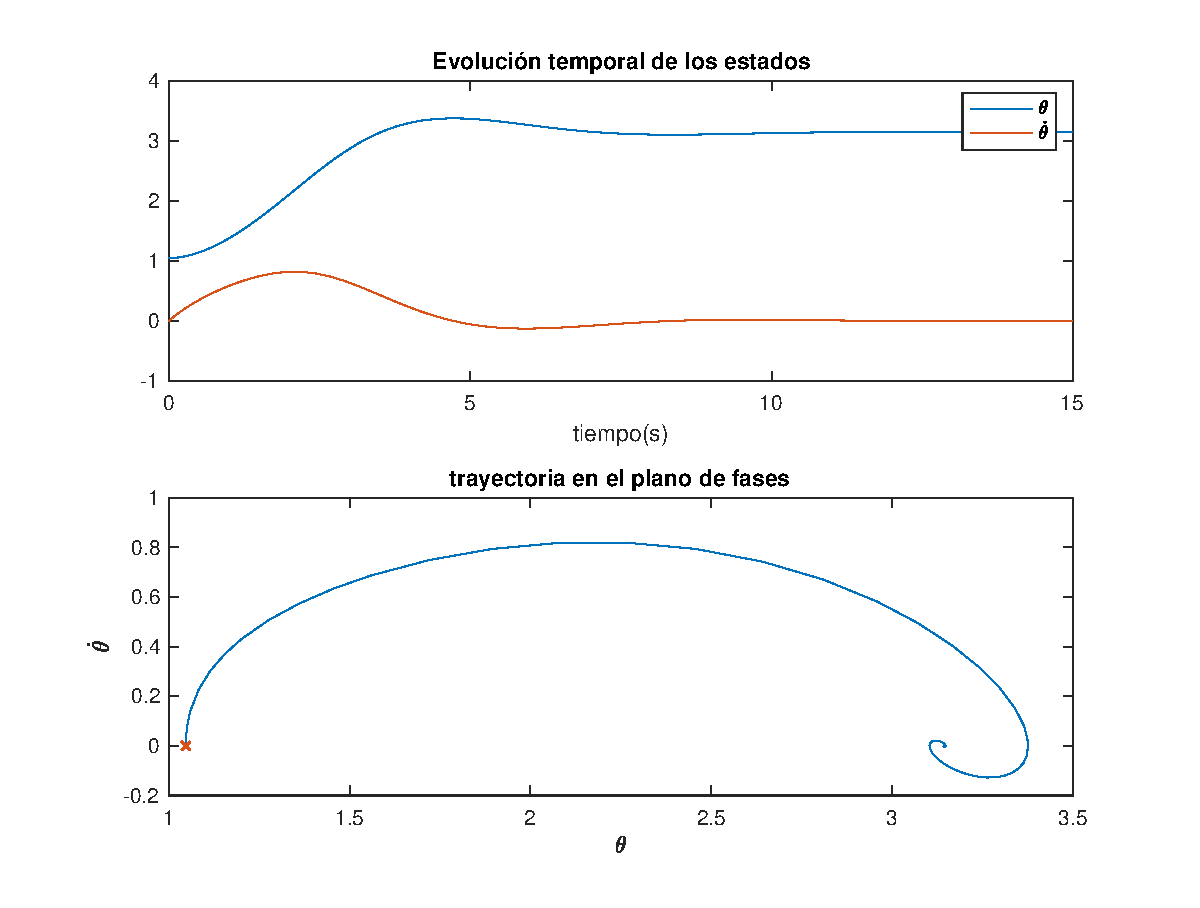
\includegraphics[scale=0.8]{resp_p_inv.eps}
\caption{Evolución temporal y trayectoria en el plano de fases para el péndulo invertido. La condición ininial, $x_0=[\pi/3,0]^T$, aparece representada con un aspa en el espacio de fases.} \label{fig:trpen}
\end{figure}

En ese caso, es fácil analizar lo que sucede, de un modo cualitativo. Las condiciones iniciales sitúan el péndulo cerca de la vertical, formando un ángulo $\theta_0 =\pi/3$ y en reposo. El péndulo caerá y oscilará con una amplitud y velocidad cada vez menor acercándose al punto de equilibrio $\overline \theta = \pi$.

Podemos obtener más información si dibujamos aproximadamente el campo vectorial definido por las ecuaciones (\ref{eq: pi1})-(\ref{eq: pi2}). La figura \ref{fig:pifield} muestra un ejemplo. La región del plano de fases $\theta \in [-3\pi/2,3\pi/2], \dot \theta \in [-3,3]$
 
\begin{figure}
\centering
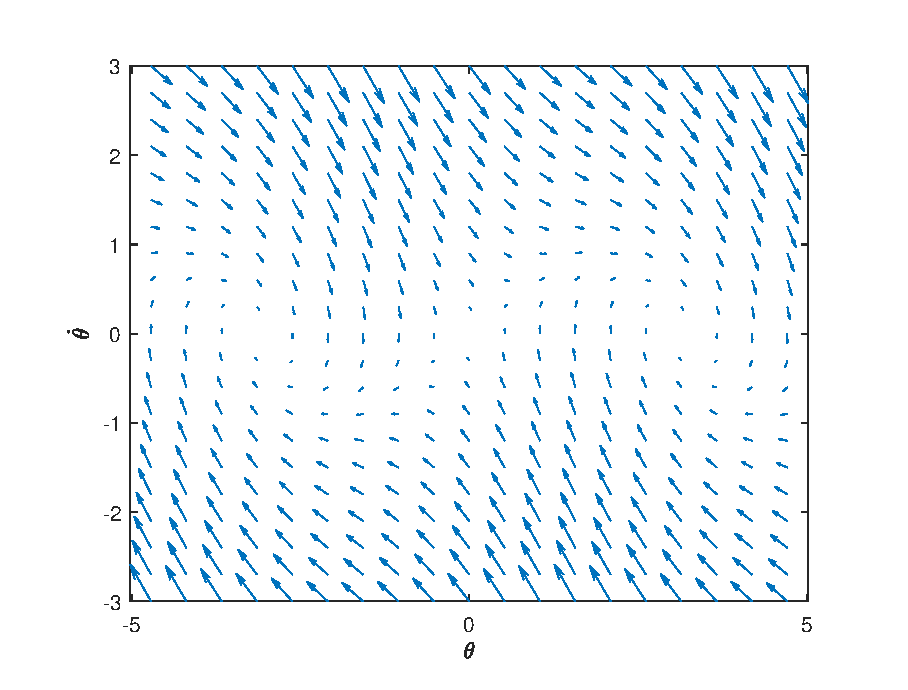
\includegraphics[scale=0.8]{pi_field.eps}
\caption{Evolución temporal y trayectoria en el plano de fases para el péndulo invertido. La condición inicial, $x_0=[\pi/3,0]^T$, aparece representada con un aspa en el espacio de fases.} \label{fig:pifield}
\end{figure}

 \begin{figure}
\centering
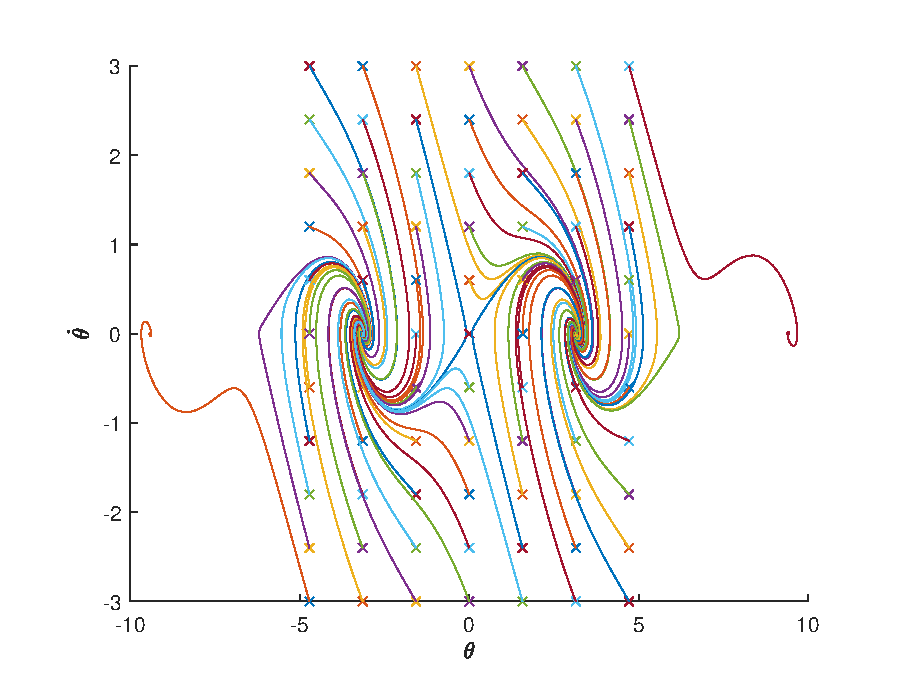
\includegraphics[scale=0.8]{pi_php.eps}
\caption{diagrama de fase para el péndulo invertido, cada aspa representa una condición inicial distinta} \label{fig:piphp}
\end{figure}
\qed
\end{example}



\chapter{Comportamiento dinámico y estabilidad}
El concepto de estabilidad y su análisis constituye unos de los aspectos claves para el estudio de los sistemas dinámicos. La estabilidad de un sistema esta estrechamente relacionada con su comportamiento dinámico y puede definirse de diversas maneras. En este capítulo nos centraremos en el análisis de los llamados puntos de equilibrio de un sistema y los estudiaremos de acuerdo con el concepto de estabilidad de Lyapunov. Además, incidiremos en otros aspectos de la estabilidad de los sistemas tales como la existencia de ciclos límite o el movimiento nominal. Empecemos pues por enunciar algunas definiciones de estabilidad.



\section{Estabilidad de un sistema dinámico}
Dado un sistema dinámico no forzado,
\begin{align}
\dot{x} = f(t,x) \label{eq: sis1}\\
y = g(t,x)
\end{align}

\begin{definition}[Estabilidad de las soluciones de un sistema dinámico]
Una solución $x(t;x_0)$ para la condición inicial $x(0) = x_0$ se dice que es estable si  $\exists R>0$ y  $ \exists r>0$ tal que, dada otra condición inicial $\hat x_0$ se verifica,
\begin{equation}
\|\hat x_0-x_0\|<r \Rightarrow \|x(t;\hat x_0) - x(t;x_0)\|<R, \forall t \geq 0
\end{equation}

En otro caso se dice que la solución es inestable 
\qed
\end{definition}

\begin{definition}[Estabilidad asintótica]
Una solución $x(t;x_0)$ para el sistema \ref{eq: sis1} se dice que es asintoticamente estable si es estable y además  $\exists r>0$, tal que dada otra condición inicial $\hat x_0$ se verifica,
\begin{equation}
\|\hat x_0-x_0\|<r \Rightarrow \lim_{t \to \infty}\|x(t;\hat x_0) - x(t;x_0)\|=0
\end{equation}

es decir, cualquier solución con condición inicial próxima  a $x(t;x_0)$ converge a $x(t;x_0)$
\qed
\end{definition}

\begin{definition}[Estabilidad marginal]
Una solución que es estable, pero asintóticamente estable, se denomina marginalmente estable
\qed
\end{definition}

\begin{definition}[Estabilidad exponencial]
Una solución $x(t;x_0)$ para el sistema \ref{eq: sis1} se dice que es exponencialmente estable estable si es estable y además  $\exists r>0$, tal que dada otra condición inicial $\hat x_0$ se verifica que existen $\alpha>0 , \sigma >0$, tales que,
\begin{equation}
\|\hat x_0-x_0\|<r \Rightarrow \|x(t;\hat x_0) - x(t;x_0)\| \leq \|\hat x_0 - x_0\| \alpha e^{-\sigma t}
\end{equation}
\qed
\end{definition}

Por último indicar que cuando la estabilidad se cumple para cualquier condición inicial, $\hat x  \in \mathbb{R}^n$ la solución $x(t;x_0)$ se denomina \emph{globalmente} estable.


\subsection{Puntos de equilibrio} 
\begin{definition}[Punto de equilibrio] Dados un sistema dinámico definido por las ecuaciones,
\begin{align}
\dot{x} = f(x,u)\\
y = g(x,u)
\end{align}
donde $x \in \mathbb{R}^n$, $u \in \mathbb{R}^m$ e $y \in \mathbb{R}^l$. Se definen como puntos de equilibrio o puntos estacionarios los valores del vector de estados $\overline x$ y del vector de entradas $\overline u$ para los cuales el estado y, consecuentemente, la salida del sistema permanecen constantes,

\begin{align}
\dot{\overline x} \equiv 0 = f(\overline x, \overline u)\\
\overline y = g(\overline x,\overline u)
\end{align}
\qed
\end{definition}

Si el vector de estados no cambia, su derivada será cero. Por tanto, mientras no se altere el valor de la entrada, el sistema permanecerá en el mismo estado y el valor del vector de salidas permanecerá también constante. 

Podemos, a partir de esta definición, obtener algunas propiedades importantes de los puntos de equilibrio:
\begin{enumerate}
\item Una vez que un sistema alcanza un punto de equilibrio, permanece en él indefinidamente. (Todas las derivadas temporales de las componentes del vector de estado son cero.
\item Desde el punto de vista del control de sistemas, los puntos de equilibrio juegan un papel importante ya que representan condiciones de operación constante.
\item Un sistema dinámico puede tener uno o más puntos de equilibrio, o no tener ninguno. 
\end{enumerate}

\paragraph{Sistemas autónomos.} Para simplificar el estudio de la estabilidad, podemos empezar por considerar el casos de sistemas autónomos con entrada nula  $u = 0, \ \forall t$. La salida evoluciona a partir de un estado inicial $x_0\equiv x(t_0)$,

\begin{align}
\dot{x} = f(x)\\
y = g(x)
\end{align}

\paragraph{Sistemas realimentados.} Del mismo modo, podemos considerar sistemas en los que la entrada es una función directa del valor de los estados; $\textbf{u}= \textbf{c(x)}$. Hablaremos entonces de un \emph{sistema realimentado}. A efectos de análisis de la estabilidad del sistema, no hay diferencia entre un sistema realimentado y un sistema autónomo,
\begin{align}
\dot{x} = f(x,c(x)) = \bar{f}(x)\\
y = g(x,c(x)) = \bar{g}(x)
\end{align}
El nombre de sistema realimentado, proviene de considerar que se están \emph{realimentando} los estados en la entrada del sistema. El concepto de realimentación constituye uno de los pilares de los sistemas de control. La figura \ref{fig:rea}, muestra esquemáticamente este concepto.

\begin{figure}
\centering
\begin{tikzpicture}
\draw(0,0) node(p)[rectangle, minimum height=10mm, minimum width=10mm,align=center, very thick, draw = blue!50!black!50]{$\mathbf{f}(\mathbf{x}(t),\mathbf{u}(t))$}

(0,-1.5) node(c)[rectangle, minimum height=10mm, minimum width=10mm,align=center ,very thick,draw = red!60!black!40]{$\mathbf{k}(\mathbf{x}(t))$};

\draw[line width = 1pt](p)--(2,0)node[midway,above]{$\mathbf{x}(t)$};
\draw[line width = 1pt](2,0)--(2,-1.5);
\draw[line width = 1pt, -latex](2,-1.5)--(c);
\draw[line width = 1pt](c)--(-2,-1.5);
\draw[line width = 1pt](-2,-1.5)--(-2,0);
\draw[line width = 1pt, -latex](-2,0)--(p)node[midway,above]{$\mathbf{u}(t)$};

\end{tikzpicture}

\caption{Esquema general de un sistema realimentado}\label{fig:rea}
\end{figure}

\section{Estabilidad de Lyapunov}
 En esta sección vamos a centrarnos en el estudio de la estabilidad de los puntos de equilibrio. 

Habitualmente, cuando se trata de la estabilidad de los puntos de equilibrio se suele hablar de estabilidad en el \emph{sentido} de Lyapunov. Aleksandr Mikhailovich Lyapunov un matématico ruso, de finales del siglo XIX, que estableció los fundamentos de la teoría de la estabilidad que ahora lleva su nombre.

Un punto de equilibrio de un sistema dinámico es \emph{estable} si toda  solución que comienzan cerca del punto de equilibrio permanece cercana al punto de equilibrio; en otro caso, el punto de equilibrio es inestable. Es \emph{asintóticamente estable} si toda solución que empieza próxima al punto de equilibrio no solo permanecen cerca del punto de equilibrio sino que tienden a él cuando el tiempo tiende a infinito.

Podemos relacionar directamente la estabilidad de un punto de equilibrio, con la estabilidad de las trayectorias de un sistema lineal definida en () i consideramos  un punto de equilibrio como una solución del sistema dinámico, cuya condición inicial es el propio punto de equilibrio: $x(t;\overline x) = \overline x$.

\subsection{Estabilidad de Lyapunov para sistemas autónomos}
Consideremos un sistema autónomo genérico,
\begin{equation}\label{eq: aut}
\dot x = f(x),
\end{equation}
donde $f(x): D\rightarrow \mathbb{R}^n$ es una función (localmente) lipschitziana desde un domino $D \subset \mathbb{R}^n$ a $\mathbb{R}^n$. Supongamos además que $\overline x \in D$ es un punto de equilibrio; es decir, $f(\overline x) = 0$. Lo que buscamos es un método para caracterizar el tipo de estabilidad de $\overline x$. En lo que sigue, y sin perdida de generalidad, consideramos que el punto de equilibrio es es origen de coordenadas $\overline x = 0$ \footnote{Siempre es posible hacer un cambio de coordenadas de modo que si $\overline x \neq 0$, $z = x-\overline x$; $\dot z = \dot x = f(x+\overline x) := g(z)$, donde $g(0)=0$.}.

\begin{definition} \label{def: est}
El punto de equilibrio x = 0 del sistema \ref{eq: aut} es:
\begin{itemize}
\item estable $\forall \epsilon > 0$ que cumpla:
\begin{equation*}
 \exists \delta =\delta(\epsilon)>0: \| x(0) \| < \delta \Rightarrow \| x(t)\| < \epsilon \ \forall t \ge 0
\end{equation*}
 
 \item Es inestable si no es estable.
 \item Es asintóticamente estable si es estable y además se puede elegir $delta$ de modo que,
\begin{equation*}
\| x(0)\| < \delta \Leftarrow \lim_{t \to \infty} x(t) = 0
\end{equation*}
\end{itemize}
\qed
\end{definition}

En 1892 Lyapunov propuso un método para analizar la estabilidad de un punto de equilibrio, basado en el análisis  una función $V:D\to \mathbb{R}$, continua y diferenciable en un entorno $D \subset \mathbb{R}^n$. En concreto, el método analiza la variación de la función $V$ a lo largo de las \emph{trayectorias} del sistema cuya estabilidad se quiere analizar, Podemos representar dicha variación empleando la derivada temporal de la función $V$
\begin{equation} \label{eq: dlyap}
\dot V(x) = \sum_{i=0}^{n}\frac{\partial V}{\partial x_i} \dot x_i = \sum_{i=0}^{n}\frac{\partial V}{\partial x_i} f(x) = \frac{\partial V}{\partial x}f(x)
\end{equation}

Es interesante hacer notar que, lógicamente, $\dot V$ depende del sistema que se desea analizar y que Si $\phi(t;x)$ es una solución del sistema \ref{eq: aut} , que empieza, como condición inicial, en estado $x$, para $t=0$ Entonces,
\begin{equation}
\dot V(x) =\left. \frac{d}{dt}V(\phi (t;x))\right|_{t=0},
\end{equation}
Por tanto, si $\dot V(x)$ es negativa, $V$ decrecerá a lo largo de la solución del sistema \ref{eq: aut}.

\begin{theorem}\label{th: lyap1}
Sea $x=0$ un punto de equilibrio para el sistema \ref{eq: aut} y $D \subset \mathbb{R}^n$ un dominio que contiene a $x=0$. Sea $V:D 	\to \mathbb{R}$ una función continua y diferenciable tal que,
\begin{equation}\label{eq: lyap1}
V(0) = 0\ y\ V(x) > 0\ en\  D-\{0\},
\end{equation}
\begin{equation}\label{eq: lyap2}
\dot V(x) \leq 0\ en\ D,
\end{equation} 
entonces $x=0$ es estable de forma local. Además, si
\begin{equation}\label{eq: lyap3}
\dot V(x) < 0 \ en\ D-\{0\},
\end{equation} 
Entonces $x(0)$ es asintóticamente estable de forma local.
\end{theorem}
\begin{proof}
Dado $\epsilon > 0$, elegimos $r \ in (0,\epsilon]$ tal que,
\begin{equation*}
B_r = \left\{ x \in \mathbb{R} \ |\  \|x\| \leq r \right\} \subset D.
\end{equation*}
Sea $\alpha =  \min_{\|x\| = r}V(x)$. Donde, $\alpha >0$ de acuerdo con \ref{eq: lyap1}. Tomamos ahora $\beta \in (0,\alpha)$ y construimos un nuevo dominio de modo que,
\begin{equation*}
\Omega_\beta = \left\{ x \in B_r \ |\  V(x) \leq \beta \right\}
\end{equation*}
Pero entonces $\Omega_\beta$ está en el interior de $B_r$.  Si no fuera así, sería posible encontrar un $p \in \Omega_\alpha$ que estaría situado en la frontera $B_r$. Pero en este punto $V(p) \ge \alpha > \beta$, lo que estaría en contradicción con la definición de $\Omega_\beta$. 

El conjunto $\Omega_\beta$ tiene la propiedad, de que cualquier trayectoria del sistema que empiece en $\Omega_\beta$  en $t=0$ permanecerá en $\Omega_\beta, \forall t \geq 0$; ya que, de acuerdo con \ref{eq: lyap2}
\begin{equation*}
\dot V \leq 0 \Rightarrow V(x(t)) \leq V(x(t)) \leq \beta, \forall t \geq 0.
\end{equation*}

Como $V(x)$ es continua y $V(0) = 0$,

\begin{equation*}
\exists \delta > 0\  |\  \|x\| \leq \delta \Rightarrow V(x) < \beta
\end {equation*}

la que implica que,
\begin{equation}
B_\delta \subset \Omega_\beta \subset B_r
\end{equation}
y
\begin{equation*}
x \in B_\delta \Rightarrow x(0) \in \Omega_\beta \Rightarrow x(t) \in B_r,
\end{equation*}
por tanto,
\begin{equation*}
\|x(0)\| < \delta \Rightarrow \|x(t)\|<r \leq \epsilon, \ t \geq 0
\end{equation*}

Lo cual demuestra que el punto $x=0$ es estable (ver definición: \ref{def: est}). 

Si además suponemos que se cumple \ref{eq: lyap3}, para demostrar que el sistema es asintóticamente estable, debemos probar que $x \to 0$ cuando $t \to \infty$; Condición que podemos reformular como, $\forall a >0, \exists T>0\ | \ \|x\| < a \ \forall t>T$. Pero, si repetimos nuestro razonamiento anterior, dato un valor $a>0$ siempre podremos encontrar un $b>0$ para el que se cumpla que $ \Omega_b \subset B_a$. Por tanto, es suficiente probar que $V$ alcanza el valor $0$ si nos movemos a lo largo de las trayectorias del sistema, $\lim_{t \to 0}V(x(t))=0$. Sabemos que $V(x(t))$ es monótona decreciente a lo largo de las trayectorias, y que está acotada inferiormente por cero.
\begin{equation}
\lim_{t \to 0}V(x(t)=c \geq 0
\end{equation}
Debemos demostrar que,  si se cumple \ref{eq: lyap3}, $c=0$. Vamos  demostrarlo por contradicción. Supongamos que $c>0$. Por continuidad de la función $V(x)$, $\exists d>0\ | \ B_d \subset \Omega_c$ pero entonces el límite $V(x(t))\to c>0$ implica que las trayectorias $x(t)$ se quedan fuera de la bola $B_d, \forall t \geq 0$. Si fijamos  un entorno $d \leq \|x\| \leq r$ exterior a $B_b$, $\dot V(x)$ deberá alcanzar un valor máximo, $-\gamma =\max_{d \leq \| x \| \leq r} \dot{V}(x)$. Además, por \ref{eq: lyap3} $-\gamma < 0$. Si integramos $\dot V$,
\begin{equation*}
V(x(t)) = V(x(0)) + \int_0^t \dot V(x(\tau))d\tau \leq V(x(0)) -\gamma t
\end{equation*}
Pero la expresión a la derecha del menor o igual, terminará por hacerse negativa, por lo que $c$ no puede ser mayor que 0.
\end{proof}
Algunas observaciones,
\begin{itemize}
\item Una función continua y diferenciable $V(x)$ que cumple las condiciones \ref{eq: lyap1} y \ref{eq: lyap2} recibe el nombre de función de Lyapunov.
\item La derivada $\dot V$, definida en la ecuación (\ref{eq: dlyap}) recibe el nombre de derivada de Lyapunov o derivada de Lie.
\item Una función $V(x)$ que satisface $V(0)=0$ y $V(x)>0$ para $x\neq 0$ en $D$, (\ref{eq: lyap1}), se dice que es definida positiva en $D$.Si la solo satisface $V(x)\geq 0$ para $x\neq 0$ en $D$, se dice que es semidefinida positiva en $D$.
\item Una función que cumple que $-V(x)$ es definida positiva/semidefinida positiva en $D$, se dice que es definida negativa/semidefinida negativa en $D$. Podríamos por tanto reescribir el teorema \ref{th: lyap1} diciendo que el origen es un punto de equilibrio estable, para un sistema dinámico si existe una función diferenciable definida positiva $V(x)$ tal que $\dot V(x)$ es semidefinida negativa, y es asintóticamente estable si $\dot V(x)$ es definida negativa.
\item El teorema \ref{th: lyap1} aporta condiciones suficientes para la estabilidad de un sistema; el hecho de no ser capaz de encontrar una función de Lyapunov para un sistema dado, no implica necesariamente que este sea inestable. 
\item Además, no es constructivo; indica que si existe una función de Lyapunov para el sistema, éste es estable, pero no indica cómo construir dicha función. 
\end{itemize}







\section{Principio de invarianza de LaSalle}


\chapter{Diseño de controladores para sistemas en el espacio de estados}

\section{Seguidor de trayectorias deseadas}
Considera el sistema $\Sigma$ en (\ref{eq: sigma}). Dada una señal deseada o trayectoria $x^*(t)\in\mathbb{R}^n$, nuestro objetivo es diseñar $u(t)\in\mathbb{R}^k$ tal que $x(t) \to x^*(t)$ para $t\to\infty$.

Para ello vamos a construir la función de error
\begin{equation}
	e(t) := x(t) - x^*(t),
\end{equation}
junto con la siguiente función candidata de Lyapunov
\begin{equation}
	V(t) = \frac{1}{2}||e(t)||^2,
	\label{eq: lyaE}
\end{equation}
cuya derivada temporal satisface
\begin{equation}
	\frac{\mathrm{d}V}{\mathrm{dt}} = e^T\dot e = e^T\big(\dot x(t) - \dot x^*(t)\big) = e^Tf(x,u) - e^T \dot x^*(t).
\end{equation}
Podemos garantizar que $e(t)\to 0$ cuando $t\to\infty$ si para un conjunto compacto $\mathcal{B} := \{e : ||e|| \leq \rho, \, \rho\in\mathbb{R}_+ \}$ tenemos que $\frac{\mathrm{d}V}{\mathrm{dt}} < 0$ si $e\in\mathcal{B} \setminus \{0\}$ y $\frac{\mathrm{d}V}{\mathrm{dt}} = 0$ si $e = 0$.

\subsection{Ejemplo con un sistema cinemático de segundo orden}
Considera el siguiente sistema cinemático de segundo orden
\begin{equation}
	\ddot p(t) = u,
	\label{eq: pdyn}
\end{equation}
donde $p,u\in\mathbb{R}^n$ son las \emph{posiciones} y las \emph{aceleraciones} respectivamente en un espacio $l\in\mathbb{N}$-dimensional. Vamos a particularizar para $l=2$. Apilamos las posiciones y velocidades $p_x,p_y,\dot p_x$ y $\dot p_y$ en $x\in\mathbb{R}^4$, consideramos que podemos medir $x$, y apilamos las aceleraciones $\ddot p_x$ y $\ddot p_y$ en $u\in\mathbb{R}^2$. Por lo que las funciones $f$ y $g$ del sistema $\Sigma$ (\ref{eq: sigma}) son
\begin{equation}
	\begin{cases}
		f &= \begin{bmatrix}0 & 1 & 0 & 0 \\ 0 & 0 & 0 & 0 \\
		0 & 0 & 0 & 1 \\ 0 & 0 & 0 & 0 \end{bmatrix} x + \begin{bmatrix}0 & 0  \\ 1 & 0  \\ 0 & 0 \\ 0 & 1\end{bmatrix} u \\
			g &= x.
\end{cases}
\end{equation}

Definimos como trayectorias deseadas para seguir
\begin{equation}
	p^*(t) = f(t), \quad \dot p^*(t) = f'(t),
\end{equation}
donde $f(t) \in C^2$.
Vamos a construir las siguientes señales de error
\begin{equation}
	e_1(t) = p(t) - p^*(t), \quad e_2(t) = \dot p(t) - \dot p^*(t),
\end{equation}
	para definir la siguiente función candidata de Lyapunov al estilo de (\ref{eq: lyaE}).
\begin{equation}
	V(e(t)) = \frac{1}{2}||e(t)||^2,
	\label{eq: Ve}
\end{equation}
	en donde $e(t)\in\mathbb{R}^4$ hemos apilado $e_1$ y $e_2$. La derivada temporal de ($\ref{eq: Ve}$) satisface
\begin{align}
	\frac{\mathrm{d}V}{\mathrm{dt}} &= e^T\dot e = e_1^T\dot e_1 + e_2^T\dot e_2 =  e_1^T(\dot p - f'(t)) + e_2^T(u - f''(t)) \nonumber \\
	&= e_1^Te_2 + e_2^T(u - f''(t))
\end{align}
por lo que si uno escoge
	\begin{equation}
	u = f''(t) - e_1 - e_2 = f''(t) - p(t) + f(t) -\dot p(t) + f'(t),
	\label{eq: ue}
	\end{equation}
nos lleva a
	\begin{equation}
\frac{\mathrm{d}V}{\mathrm{dt}} = -||e_2||^2 \leq 0.
	\end{equation}
	De hecho, la derivada temporal de $V(t)$ es cero sí y solo sí $e_2 = 0$. Por lo que para invocar al principio de invariance de LaSalle, debemos comprobar cual es el conjunto invariante más grande del sistema (autónomo) error $\dot e$ cuando $e_2 = 0$, esto es,
	\begin{equation}
	\begin{cases}
	\dot e_1 &= e_2 \\
	\dot e_2 &= -e_1 -e_2
	\end{cases},
	\end{equation}
	donde se puede ver que cuando $e_2 = 0$, el conjunto invariante más grande es $e_1 = e_2 = 0$. Consecuentemente, podemos concluir que $e(t) \to 0$ cuando $t\to\infty$ para cualquier $e(0)$ empezando en $\mathcal{B}$ con un $\rho$ arbitrario, esto es, tenemos convergencia global.

	\section{Diseño de ciclos límites para sistemas planos}
	Consideremos de nuevo el sistema (\ref{eq: pdyn}) para $l=2$, es decir, seguimos en 2D, o un sistema en el plano. En vez de querer seguir una trayectoria $p^*(t)$, queremos que la posición converja a un \emph{camino} cerrado que además sea un ciclo límite. El camino cerrado lo podemos definir como una curva $\phi(p_x, p_y) = 0$, es decir, todos los puntos con curva de nivel igual a cero definen \emph{el camino}. Por ejemplo, un círculo de radio $r\in\mathbb{R}_+$ 
 satisface
	\begin{equation}
	\phi(p) := p_x^2 + p_y^2 - r^2 = 0.
	\end{equation}
Atención a que podemos considerar $\phi(p)$ como una señal de error, i.e., $e(t) := \phi(p(t))$. Consecuentemente, podemos definir la siguiente función candidata de Lyapunov.
\begin{equation}
	V(e(t)) = \frac{1}{2}e(t)^2 + \frac{1}{2}||\dot p(t) - \dot p^*(t)||^2,
	\label{eq: Ve2}
\end{equation}
	cuya derivada temporal satisface (por ahora considera $\dot p^*(t) = 0$).
	\begin{equation}
		\frac{\mathrm{d}V}{\mathrm{dt}} = e\dot e + \dot p^T\ddot p = e \nabla\phi(p) \dot p + \dot p^T u,
	\end{equation}
	entonces, si uno escoge $u = -e \nabla\phi(p)^T -\dot p$, entonces tenemos que
	\begin{equation}
\frac{\mathrm{d}V}{\mathrm{dt}} = -||\dot p||^2 \leq 0,
	\end{equation}
y, similarmente a como hemos hecho en la sección anterior, por el principio de invarianza de LaSalle's concluimos que $e(t) \to 0$ cuando $t\to\infty$.

\subsection{Ejercicio}
Para que $\phi(p)$ sea un ciclo límite, la posición no solo ha de converger a ese camino, sino que ha de evolucionar en él en el tiempo. Para ello considera $\dot p^*(t) = \begin{bmatrix}0 & 1 \\ -1 & 0\end{bmatrix}\nabla\phi(p)^T$, y concluye que ahora $\phi(p)$ sí es un ciclo límite.


\chapter{Sistemas lineales}\label{chap5}

\section{Mapas lineales}

En este capítulo nos vamos a centrar en una clase de sistema llamado \emph{sistema linea en el espacio de estados}. Primero, necesitamos la noción de que es un \emph{mapa lineal}.

\begin{definition} Considera un mapeado $H: V \to W$. Si $H$ preserva la operación suma y la multiplicación por un escalar, i.e.,
\begin{align}
	H(v_1+v_2) &= H(v_1) + H(v_2), \quad v_1, v_2\in\mathbb{V} \nonumber \\
	H(\alpha v_1) &= \alpha H(v_1), \quad \alpha\in\mathbb{K} \nonumber,
\end{align}
	entonces $H$ es un \emph{mapa lineal}.
\end{definition}

\subsection{Ejercicio: Comprueba si los siguientes mapas son lineales}

\begin{enumerate}
	\item $H_1(v) := Av, A\in\mathbb{R}^{n\times n}, \quad v\in\mathbb{R}^n$
	\item $H_2(v) := \frac{\mathrm{d}}{\mathrm{dt}}(v(t)), \quad v\in\mathcal{C}^1$
	\item $H_3(v) := \int_0^T v(t) dt, \quad v\in\mathcal{C}^1, T\in\mathbb{R}_{\geq 0}$
	\item $H_4(v) := D(v) := v(t - T), \quad v\in\mathcal{C}^1, T\in\mathbb{R}_{\geq 0}$
	\item $H_5(v) := Av + b, \quad A\in\mathbb{R}^{n\times n}, v,b\in\mathbb{R}^n$
\end{enumerate}

\section{Sistemas continuos y lineales en el espacio de estados}

El siguiente sistema define un sistema continuo y lineal en el espacio de estados.

\begin{equation}
	\Sigma := \begin{cases}
	\dot x(t) &= A(t)x(t) + B(t)u(t), \quad x\in\mathbb{R}^n, u\in\mathbb{R}^k \\
	y(t) &= C(t)x(t) + D(t)u(t), \quad y\in\mathbb{R}^m
	\end{cases}
	\label{eq: linsys}
\end{equation}

\subsection{Ejercicio: Escribe un sistema continuo y lineal en el espacio de estados como un diagrama de bloques entrada/salida y comprueba que es un mapa lineal.}

\subsection{Ejercicio: Interconecta sistemas continuos y lineales en el espacio de estados y comprueba que el sistema resultante es otro sistema continuo y lineal en el espacio de estados.}

Reescribe como un único sistema lineal\footnote{Por abreviar, cuando no exista ambiguedad, llamaremos sistema lineal al sistema continuo y lineal en el espacio de estados} como en (\ref{eq: linsys}):

\begin{enumerate}
	\item La conexión en serie (o en cascada) de dos sistemas lineales, i.e., $y_1(t) = u_2(t)$.
	\item La conexión en paralelo de dos sistemas lineales, i.e., $y(t) = y_1(t) + y_2(t)$.
	\item La conexión realimentada, i.e., $u_1(t) = u(t) - y(t)$, asumiendo que $u, y, \in\mathbb{R}^k$.
\end{enumerate}

\begin{figure}
\centering
\begin{tikzpicture}[auto, node distance=3.5cm, >=latex']
	\node [input, name=input] {};
	\node [block, right of=input] (system) {$\Sigma_1$};
	\node [output, right of=system] (output) {};
	\draw [draw,->] (input) -- node {$u(t) = u_1(t)$} (system);
	\draw [->] (system) -- node [name=y] {$y_1(t)$}(output);
	\node [block, right of=output] (system2) {$\Sigma_2$};
	\node [output, right of=system2] (output2) {};
	\draw [draw,->] (output) -- node {$u_2(t)$} (system2);
	\draw [->] (system2) -- node [name=y] {$y_2(t) = y(t)$}(output2);
\end{tikzpicture}
	\caption{Conexión en serie de dos sistemas lineales y continuos en el espacio de estados.}
	\label{fig: series}
\end{figure}

\section{Solución a sistemas continuos lineales en el espacio de estados}
La solución a una ecuación diferencial ordinaria viene dada por la suma de dos soluciones: la solución a la parte homogénea, y la solución a la parte no homogénea.

\begin{equation}
	\dot x(t) = \underbrace{A(t)x(t)}_{\text{homogénea}} + \underbrace{B(t)u(t)}_{\text{no homogénea}}
	\label{eq: xdyn}
\end{equation}

\begin{theorem}{Serie de Peano-Barker.}
La solución única al sistema homogéneo $\dot x = Ax$ viene dada por
	\begin{equation}
		x(t) = \Phi(t,t_0)x(t_0), \quad x(t_0)\in\mathbb{R}^n, t\geq 0,
	\end{equation}
donde
	\begin{align}
		\Phi(t,t_0) := I + \int_{t_0}^t A(s_1)ds_1 + \int_{t_0}^t A(s_1) \int_{t_0}^{s_1} A(s_2)ds_2ds_1 \nonumber \\ + \int_{t_0}^t A(s_1) \int_{t_0}^{s_1} A(s_2)\int_{t_0}^{s_2} A(s_3) ds_3ds_2ds_1 + \dots . \label{eq: ser}
	\end{align}
\end{theorem}
Esbozo de la prueba: \\
Primero calculamos la siguiente derivada
	\begin{align}
		\frac{d}{dt}\Phi(t,t_0) &= A(t) + A(t)\int_{t_0}^{t}A(s_2)ds_2 \nonumber \\ &+ A(t)\int_{t_0}^t A(s_2) \int_{t_0}^{s_2} A(s_3)ds_3ds_2 + \dots \nonumber \\
		&= A(t) \Phi(t,t_0).
	\end{align}
	Afirmamos que la solución a la parte homogénea de (\ref{eq: xdyn}) es $x(t) = \Phi(t,t_0)x_0$ cuya derivada con respecto al tiempo es
\begin{align}
	\frac{d}{dt} x &= \frac{d}{dt}\Phi(t,t_0)x_0 \nonumber \\
	&= A(t) \Phi(t,t_0) x_0 \nonumber \\
	&= A(t)x(t),
\end{align}
lo cual prueba la identidad $\dot x = A(t)x(t)$ dado que $x(t) = \Phi(t,t_0)x_0$. Para terminar la prueba, necesitaríamos probar que la serie (\ref{eq: ser}) converge para todo $t\geq t_0$.

La matriz $\Phi(t,t_0)$ es llamada \textbf{\emph{matriz de transición de estados}}. Dada una condición inicial $x_0$, podemos predecir $x(t)$ en (\ref{eq: xdyn}) iterando $\Phi(t,t_0)$ en el caso de que no existiera ninguna interacción con el sistema, i.e., $u(t) = 0, t\geq t_0$.

\subsection{Ejercicio}
Comprobar que
\begin{align}
	x(t) &= \Phi(t,t_0)x_0 + \int_{t_0}^t \Phi(t,\tau)B(\tau)u(\tau)d\tau  \label{eq: solx} \\
	y(t) &= C(t)\phi(t,t_0)x_0 + \int_{t_0}^t C(t)\Phi(t,\tau)B(\tau)u(\tau)d\tau + D(t)u(t), \label{eq: soly}
\end{align}
son las soluciones a

\begin{align}
	\dot x(t) &= A(t)x(t) + B(t)u(t)  \nonumber \\
	y(t) &= C(t)x(t) + D(t)u(t).  \nonumber
\end{align}

\section[Solución a sistemas LTI en el espacio de estados]{Solución a sistemas invariantes en el tiempo, continuos y lineales en el espacio de estados}\label{5:lti}

Comunmente conocidos como sistemas \emph{lti} (linear time invariant), son los sistemas en los que nos centraremos principalmente en el resto del curso. La matriz $\Phi(t,t_0)$ puede ser hallada analíticamente cuando $A$ es una matriz de coeficientes constantes. Si $A$ es constante, entonces podemos sacarla de las integrales en (\ref{eq: ser}), quedando
\begin{align}
	\Phi(t,t_0) := I + A \int_{t_0}^t ds_1 + A^2 \int_{t_0}^t \int_{t_0}^{s_1} ds_2ds_1 \nonumber \\ + A^3 \int_{t_0}^t \int_{t_0}^{s_1} \int_{t_0}^{s_2} ds_3ds_2ds_1 + \dots \label{eq: phi},
\end{align}
y observando que las siguientes integrales tienen solución analítica
\begin{align}
	\int_{t_0}^t ds_1 &= (t-t_0) \nonumber \\
	\int_{t_0}^t\int_{t_0}^{s_1} ds_2ds_1 &= \frac{(t-t_0)^2}{2} \nonumber \\
	\vdots \nonumber \\
	\int_{t_0}^t\int_{t_0}^{s_1} \cdots \int_{t_0}^{s_{k-2}}\int_{t_0}^{s_{k-1}}ds_k ds_{k-1} \cdots ds_2ds_1 &= \frac{(t-t_0)^k}{k!}, \nonumber
\end{align}
entonces tenemos que (\ref{eq: phi}) es calculada como
\begin{equation}
	\Phi(t,t_0) = \sum_{k=0}^{\infty} \frac{(t-t_0)^k}{k!}A^k,
\end{equation}
lo cual es familiar a la serie de Taylor de una función exponencial. Por ejemplo, para un escalar $x$, tenemos que $e^x := \sum_{k=0}^{\infty}\frac{1}{k!}x^k = 1 + x + \frac{x^2}{2} + \frac{x^3}{3!} + \dots $. De hecho, la definición de la \emph{exponencial de una matriz} es
\begin{equation}
	exp(A) = I + A + \frac{1}{2} A^2 + \frac{1}{3!} A^3 + \dots
\end{equation}
Fijemos $t_0 = 0$ por conveniencia, entonces
\begin{align}
	\Phi(t,0) &= I + tA + \frac{t^2}{2} A^2 + \frac{t^3}{3!} A^3 + \dots \nonumber \\
	&= exp(At),
\end{align}
por lo tanto, la solución a la parte homogénea (\ref{eq: xdyn}) teniendo $A$ con coeficientes constantes y fijando $t_0 = 0$ es
\begin{equation}
	x(t) = exp(At)x_0,\quad t\geq 0.
	\label{eq: xexp}
\end{equation}

Para continuar, necesitamos el siguiente resultado de álgebra lineal.
\begin{theorem}
\textbf{Forma de Jordan}. Para una matriz cuadrada $A\in\mathbb{C}^{n \times n}$, existe un cambio de base no singular $P\in\mathbb{C}^{n \times n}$ que transforma $A$ en
\begin{equation}
	J = PAP^{-1} = \begin{bmatrix}
		J_1 & 0 & 0 & \dots & 0 \\
		0 & J_2 & 0 & \dots & 0 \\
		0 & 0 & J_3 & \dots & 0 \\
		\vdots & \vdots & \vdots & \cdots & \vdots \\
		0 & 0 & 0 & \cdots & J_l
	\end{bmatrix},
\end{equation}
donde $J_i$ es el bloque de Jordan con forma
	\begin{equation}
	J_i = \begin{bmatrix}
\lambda_i & 1 & 0 & \dots & 0 \\
		0 & \lambda_i & 1 & \dots & 0 \\
		0 & 0 & \lambda_i & \dots & 0 \\
		\vdots & \vdots & \vdots & \cdots & \vdots \\
		0 & 0 & 0 & \cdots & \lambda_i
	\end{bmatrix}_{n_i\times n_i},
	\end{equation}
	en donde cada $\lambda_i$ es un autovalor de $A$, y el número $l$ de bloques de Jordan es igual al número total de autovectores independientes de $A$. La matrix $J$ es única (descontando reordenación de filas/columnas) y es llamada la \textbf{forma normal de Jordan} de $A$.
\end{theorem}

Partiendo de la observación que $A = P^{-1}JP$ también, entonces es fácil probar que 
\begin{equation}
	A^k = P^{-1} J^k P,
\end{equation}
de tal manera que podamos calcular que
\begin{align}
	exp(At) &= P^{-1}\left(\sum_{k=1}^\infty \frac{t^k}{k!} \begin{bmatrix}J_1^k & 0 & \cdots & 0 \\ 0 & J_2^k & \cdots & 0 \\ \vdots & \vdots & \cdots & \vdots \\ 0 & 0 & \cdots & J_l^k \end{bmatrix} \right) P \nonumber \\
		&= P^{-1} \begin{bmatrix}exp(J_1t) & 0 & \cdots & 0 \\ 0 & exp(J_2t) & \cdots & 0 \\ \vdots & \vdots & \cdots & \vdots \\ 0 & 0 & \cdots & exp(J_lt) \end{bmatrix} P
\end{align}

Observa que si $J$ es simplemente una matriz diagonal con los autovalores de $A$, i.e., $J_l = \lambda_l \in \mathbb{C}$, entonces $exp(J_lt) = e^{\lambda_lt} \in\mathbb{C}$ es un cálculo trivial.

Now, let us check the consequencues on the following two conditions
Ahora, veamos las consecuencias de las siguientes dos suposiciones
\begin{enumerate}
	\item $J$ es diagonal.
	\item Todos los autovalores de $A$ tienen parte real negativa.
\end{enumerate}

Sabiendo que $\lim_{t\to\infty} e^{\lambda t} \to 0$ si $\lambda \in \mathbb{R}_{<0}$, entonces tenemos que $exp(At) \to 0$ según $t\to\infty$ si las dos previas suposiciones se dan. Si echamos un vistazo a (\ref{eq: xexp}), podemos concluir que 
\begin{equation}
	\lim_{t\to\infty} x(t) \to 0,
	\label{eq: xlim}
\end{equation}
por tanto, podemos predecir la evolución de $x(t)$ con sólamente mirar los autovalores de $A$. Si $J$ no es diagonal, podremos concluir más resultados. Lo veremos en la sección siguiente a la linearización de sistemas en el espacio de estados.


\section{Linearización de sistemas en el espacio de estados}\label{sec: linear}
Desafortunadamente, es realmente dificil (cuando no imposible) calcular una solución analítica para $x(t)$ e $y(t)$ para un sistema arbitrario $\Sigma$ como en (\ref{eq: sigma}). No obstante, hemos visto que sí se puede calcular una solución analítica para $x(t)$ e $y(t)$ cuando $\Sigma$ es un sistema invariante en el tiempo, continuo y lineal en el espacio de estados.

Será de gran utilidad encontrar una relación entre ambos sistemas.

Si $f(x,t)$ y $g(x,t)$ son reales analíticas en un entorno a un punto específico $(x^*,u^*)$, entonces podemos trabajar con aproximaciones de Taylor de $f(x,t)$ y $g(x,t)$ en ese mismo entorno. Cuando nos quedamos en orden uno en la aproximación es lo que se conoce como \emph{linearización}.
\begin{equation}
	\Sigma := \left.\begin{cases}
	\dot x(t) =& f(x(t),u(t)) \\ y(t) =& g(x(t),u(t))
	\end{cases}\right|_{x\approx x^*, u\approx u^*} \approx
	\begin{cases}
		x(t) &= x^* + \delta x(t) \\
		u(t) &= u^* + \delta u(t) \\
	\delta \dot x(t) &= A(t)\delta x(t) + B(t)\delta u(t) \\
	\delta y(t) &= C(t)\delta x(t) + D(t)\delta u(t)
	\end{cases}, \nonumber
\end{equation}
donde
\begin{align}
	A(t) &= \begin{bmatrix}
		\frac{\partial f_1}{\partial x_1} & \dots & \frac{\partial f_1}{\partial x_n} \\
		\vdots & \vdots & \vdots \\
		\frac{\partial f_n}{\partial x_1} & \dots & \frac{\partial f_n}{\partial x_n}
	\end{bmatrix}_{|_{x=x^*, u=u^*}} \quad
	&B(t) = \begin{bmatrix}
		\frac{\partial f_1}{\partial u_1} & \dots & \frac{\partial f_1}{\partial u_k} \\
		\vdots & \vdots & \vdots \\
		\frac{\partial f_k}{\partial u_1} & \dots & \frac{\partial f_k}{\partial u_k}
	\end{bmatrix}_{|_{x=x^*, u=u^*}} \nonumber \\
	C(t) &= \begin{bmatrix}
		\frac{\partial g_1}{\partial x_1} & \dots & \frac{\partial g_1}{\partial x_n} \\
		\vdots & \vdots & \vdots \\
		\frac{\partial g_m}{\partial x_1} & \dots & \frac{\partial g_m}{\partial x_n}
	\end{bmatrix}_{|_{x=x^*, u=u^*}} \quad
	&D(t) = \begin{bmatrix}
		\frac{\partial g_1}{\partial u_1} & \dots & \frac{\partial g_1}{\partial u_k} \\
		\vdots & \vdots & \vdots \\
		\frac{\partial g_m}{\partial u_1} & \dots & \frac{\partial g_m}{\partial u_k}
	\end{bmatrix}_{|_{x=x^*, u=u^*}}. \nonumber
\end{align}
Informalmente, estamos calculando la sensibilidad (hasta primer orden) de $f$ y $g$ cuando hacemos una variación pequeña de $x$ y $u$ alrededor de $(x^*,u^*)$. Como de pequeña ha de ser esa variación depende del sistema $\Sigma$. En particular, cuando diseñemos controladores basados en linearizar alrededor de un punto, daremos cotas para $\delta x$ y $\delta u$ de tal manera que el controlador pueda garantizar estabilidad.

\subsection{Ejercicio. Linearización del péndulo invertido}
Más adelante, veremos que podemos diseñar una entrada de control $u(t)$, i.e., una señal que ha de seguir el torque $T$ en (\ref{eq: f}) de tal manera que $\theta$ y $\dot\theta$ converjan a unos valores constantes o trayectorias deseadas.

Por ejemplo, vamos a fijar un punto constante de interés $x^* = \begin{bmatrix}\theta^* \\ 0\end{bmatrix}$, por lo que la velocidad angular se marca a cero. Esta situación corresponde a una situación de equilibrio para el ángulo $\theta$. Para hallar el $u^*(t)$ en (\ref{eq: f}) necesario para tal equilibrio necesitamos que $\frac{\mathrm{d}}{\mathrm{dt}}\left(\begin{bmatrix}\theta \\ \dot\theta \end{bmatrix}\right) = \begin{bmatrix}0 \\ 0 \end{bmatrix}$. Una inspección a la dinámica (\ref{eq: dyn}) nos responde que
\begin{equation}
	u^* = T^* = -\frac{g}{l}\sin\theta^*,
\end{equation}
por ejemplo, para una posición totalmente vertical correspondiente a $\theta^* = 0$ tenemos que $T^*=0$, i.e., $x^* = \begin{bmatrix}0\\0\end{bmatrix}$ y $u^* = 0$.

El cáclulo de las matrices $A,B,C,$ y $D$ son los Jacobianos de $(\ref{eq: f})$ y $(\ref{eq: g})$, i.e.,

\begin{align}
\frac{\partial f_1}{\partial x_1} &= 0 \nonumber \\
\frac{\partial f_1}{\partial x_2} &= 1 \nonumber \\
\frac{\partial f_2}{\partial x_1} &= \frac{g}{l}\cos\theta \nonumber \\
\frac{\partial f_2}{\partial x_2} &= -\frac{b}{ml^2} \nonumber \\
\frac{\partial f_1}{\partial u_1} &= 0 \nonumber \\
\frac{\partial f_2}{\partial u_1} &= 1 \nonumber \\
\frac{\partial g_1}{\partial x_1} &= 1 \nonumber \\
\frac{\partial g_1}{\partial x_2} &= 0 \nonumber \\
\frac{\partial g_1}{\partial u_1} &= 0, \nonumber
\end{align}
por lo que podemos llegar a
\begin{align}
	\frac{\mathrm{d}}{\mathrm{dt}}\left(\begin{bmatrix}\delta\theta \\ \dot\delta\theta \end{bmatrix}\right) &= \begin{bmatrix}0 & 1 \\ \frac{g}{l}\cos\theta & -\frac{b}{ml^2} \end{bmatrix}_{|_{\theta=\theta^*}} \begin{bmatrix}\delta\theta \\ \dot\delta\theta \end{bmatrix} + \begin{bmatrix}0 \\ 1 \end{bmatrix} \delta T \nonumber \\
		\delta y &= \begin{bmatrix}1 & 0\end{bmatrix}\begin{bmatrix}\delta\theta \\ \dot\delta\theta \end{bmatrix} + 0 \, \delta T,
\end{align}
para modelar una aproximación a la dinámica de $x(t)$ y la salida $y(t)$ alrededor de los puntos $x^*$ y $u^*$.

\begin{comment}
\section{(Internal or Lyapunov) Stability}
\label{sec: sta}

Decimos que el sistema lineal (\ref{eq: linsys}) \emph{en el sentido de Lyapunov}
\begin{enumerate}
	\item es \emph{(marginalmente) estable} si para cada condición inicial $x_0$, entonces $x(t) = \Phi(t,t_0) x_0$ está acotada uniformamente para todo $t>t_0$.
	\item es \emph{asintóticamente estable} si además $x(t) \to 0$ según $t\to\infty$.
	\item es \emph{exponencialmente estable} si además $||x(t)|| \leq c e^{\lambda(t-t_0)}||x(t_0)||$ para algunas constantes $c,\lambda > 0$.
	\item is \emph{inestable} si no es marginalmente estable.
\end{enumerate}

%In control, it is very common to focus on \emph{error signals}, e.g., $e(t) := x(t) - x^*(t)$, where $x^*(t)$ is a trajectory goal. Note that if $x^*$ is constant, then $\dot e(t) = \dot x(t)$, and this is why we focus on having $x(t) \to 0$ as $t\to\infty$ in the above definitions for (\ref{eq: sigmalin}).

Centrémonos en sistemas \emph{lti}, es decir, cuando $A$ tiene coeficientes constantes o $\Phi(t,t_0) = e^{A(t-t_0)}$. Entonces, podemos establecer una clara relación entre los autovalores de $A$ y las definiciones de estabilidad en el sentido de Lyapunov únicamente inspeccionando la solución a $\dot x(t) = Ax(t)$ dada por (\ref{eq: solx}).

El sistema $\dot x(t) = Ax(t)$
\begin{enumerate}
	\item es marginalmente estable si y solo si todos los autovalores de $A$ tienen parte real negativa. Si algún autovalor tiene parte real nula, entonces su bloque de Jordan ha de ser $1\times 1$.
	\item es asintóticamente estable si y solo si todos los autovales de $A$ tienen estrictamente parte real negativa.
	\item es exponencialmente estable si es asintóticamente estable.
	\item es inestable si y solo si al menos un autovalor de $A$ tiene parte real positiva, o al menos uno de los autovalores con parte real nula tiene un bloque de Jordan mayor de $1\times 1$.
\end{enumerate}

Comprobando las soluciones (\ref{eq: solx})-(\ref{eq: soly}), podemos decir que si $A$ tiene coeficientes constantes y $\dot x = Ax$ es asintóticamente estable, entonces $x(t) \to \int_{t_0}^t e^{A(t-\tau)}B(\tau)u(\tau)d\tau$ según $t\to\infty$. 

\subsection{Estabilidad local de sistemas linearizados}
Si $x(t)$ es asintóticamente (exponencialmente) estable en $\dot x(t) = Ax(t)$, entonces, existe una única $P$ que satisface la \emph{ecuación de Lyapunov}
\begin{equation}
A^TP + PA = -Q, \quad \forall Q \succ 0.
	\label{eq: lya}
\end{equation}
Uno puede probar (\ref{eq: lya}) si considera
\begin{equation}
	P:= \int_0^\infty e^{A^Tt}Qe^{At}dt.
	\label{eq: P}
\end{equation}
Pista: Primero, sustituye $P$ en (\ref{eq: lya}), y después verifica el cálculo  $\frac{\mathrm{d}}{\mathrm{dt}}\left(e^{A^Tt}Qe^{At}\right)$. Si uno prueba que $P$ es única, entonces $P$ ha de ser positiva definida acorde a su definición (\ref{eq: P}).

Ahora vamos a considerar un sistema continuo, autónomo y no lineal en general
\begin{equation}
	\dot x(t) = f(x(t)), \quad x\in\mathbb{R}^n,
	\label{eq: non}
\end{equation}
con un punto de equilibrio $x^*\in\mathbb{R}^n$, i.e, $f(x^*) = 0$. La dinámica de $x(t)$ puede ser aproximada considerando $x(t) = x^* + \delta x(t)$ donde 
\begin{equation}
	\dot{\delta x(t)} = A\,\delta x(t), \quad A:=\frac{\partial f(x)}{\partial x}.
	\label{eq: delta}
\end{equation}

¿Cómo de buena es esta aproximación?

\begin{theorem}
	\label{thm: tayl}
	Asume que $f(x)$ is dos veces diferenciable. Si (\ref{eq: delta}) es exponencialmente estable, entonces, existe un entorno $\mathcal{B}$ alrededor de $x^*$ y constantes $c, \lambda > 0$ tal que para cada solución $x(t)$ del sistema (\ref{eq: non}) que empiece con $x(t_0)\in\mathcal{B}$, tenemos que
	\begin{equation}
	||x(t) - x^*|| \leq ce^{\lambda(t-t_0)} ||x(t_0) - x^*||, \quad \forall t\geq t_0.
	\end{equation}
\end{theorem}

\subsubsection{¿Cómo de grande es $\mathcal{B}$? ¿Podemos estimarlo? Esbozo de la prueba del Teorema \ref{thm: tayl}}

Como $f$ es dos veces diferenciable, de su desarrollo de Taylor tenemos que
\begin{equation}
	r(x) := f(x) - (f(x^*) + A(x - x^*)) = f(x) - A\,\delta x = O(||\delta x||^2),
\end{equation}
lo cual significa que existe una constante $c$ y una bola $\bar B$ alrededor de $x^*$ tal que 
\begin{equation}
	||r(x)|| \leq c||\delta x||^2, \quad x\in\bar B.
\end{equation}
Si el sistema linearizado es exponencialmente estable, tenemos que
\begin{equation}
A^TP + PA = -I.
\end{equation}
Ahora considera la siguiente señal escalar
\begin{equation}
	v(t) := (\delta x)^T P \delta x, \quad \forall t\geq 0.
\end{equation}
Observa que $\delta x(t) = x(t) - x^*$, entonces $\dot{\delta x(t)} = \dot x(t) = f(t)$. Por lo tanto, la derivada con respecto del tiempo de $v(t)$ satisface
\begin{align}
	\dot v &= f(x)^T P \delta x + (\delta x)^T P f(x) \nonumber \\
	&= (A\delta x + r(x))^T P \delta x + (\delta x)^T P (A\delta x + r(x)) \nonumber \\
	&= (\delta x)^T(A^T P + PA)\delta x + 2(\delta x)^T P r(x) \nonumber \\
	&= -||\delta x||^2 + 2(\delta x)^T P r(x) \nonumber \\
	&\leq -||\delta x||^2 + 2 ||P||\, ||\delta x|| \, ||r(x)||.
\end{align}

Sabemos que $v(t)$ es positiva excepto cuando $\delta x = 0$. Si podemos garantizar que $\dot v(t) < 0$ y que $\dot v(t) = 0$ solo cuando  $\delta x = 0$, entonces $v(t) \to 0$ as $t\to\infty$, lo cual implica que  $\delta x(t) \to 0$ as $t\to\infty$.

Ahora, si $x\in\mathcal{\bar B}$, entonces

\begin{equation}
	\dot v \leq -\Big(1 - 2c\,||P||\,||\delta x||\Big)||\delta x||^2,
\end{equation}
Por lo tanto, si la desviación  $\delta x$ es suficientemente pequeña, i.e., 
\begin{equation}
||\delta x|| < \frac{1}{2c||P||},
\end{equation}
entonces  $\dot v(t) < 0$ si $\delta x(0) \neq 0$ y $\delta x(0) < \frac{1}{2c||P||}$.

Podemos concluir que una estimación de $\mathcal B$ es
\begin{equation}
	\mathcal{B} := \{ \delta x : ||\delta x|| < \frac{1}{2c||P||} \}.
	\label{eq: Bregion}
\end{equation}

\section{Controlabilidad}
\subsection{Subespacios alcanzables y controlables}
Recordemos que cueando aplicamos una entrada genérica $u(\cdot)$ a (\ref{eq: linsys}), transferimos el sistema de un estado $x(t_0):=x_0$ a un estado $x(t_1):=x_1$, que además podemos calcular con la expresión
\begin{equation}
	x_1 = \Phi(t_1,t_0)x_0 + \int_{t_0}^{t_1} \Phi(t_1,\tau)B(\tau)u(\tau)d\tau,
\end{equation}
donde recordemos que $\Phi(\cdot)$ es la matriz de transición de estados del sistema.

Preguntas:
\begin{enumerate}
	\item ¿Qué estados puedo alcanzar desde $x_0$?
	\item ¿Existe siempre una entrada $u(\cdot)$ que transfiera un estado arbitrario $x_0$ a otro $x_1$?
\end{enumerate}

Estas dos preguntas llevan a acuñar las definiciones de (sub)espacios alcanzables y controlables.

\begin{definition}[Subespacio alcanzable]
	Dados dos instantes de tiempo $t_1>t_0\geq 0$, el subespacio alcanzable (o controlable desde el origen) $\mathcal{R}[t_0,t_1]$ consiste en todos los estados $x_1$ por los que existe una entrada $u:[t_0,t_1]\to \mathbb{R}^k$ que transfiere el estado $x_0 = 0$ a  $x_1 \in\mathbb{R}^n$; i.e.,
	\begin{equation}
		\mathcal{R}[t_0,t_1] := \Big\{x_1\in\mathbb{R}^n : \exists u(\cdot),\, x_1 = \int_{t_0}^{t_1} \Phi(t_1,\tau)B(\tau)u(\tau)d\tau \Big\}. \label{eq: rs}
	\end{equation}
\end{definition}

\begin{definition}[Subespacio controlable]
	Dados dos instantes de tiempo $t_1>t_0\geq 0$, el subespacio controlable (or controlable hacia el origen) $\mathcal{C}[t_0,t_1]$ consiste en todos los estados $x_0$ por los que existe una entrada $u:[t_0,t_1]\to \mathbb{R}^k$ que transfiera un estado $x_0\in\mathbb{R}^n$ a $x_1 = 0$; i.e.,
	\begin{equation}
		\mathcal{C}[t_0,t_1] := \Big\{x_0\in\mathbb{R}^n : \exists u(\cdot),\, 0 = \Phi(t_1,t_0)x_0 + \int_{t_0}^{t_1} \Phi(t_1,\tau)B(\tau)u(\tau)d\tau \Big\}.
	\end{equation}
\end{definition}

¿Cómo podemos calcular $\mathcal{R}[t_0,t_1]$ y $\mathcal{C}[t_0,t_1]$? Para ello vamos a introducir y explotar las siguientes dos matrices llamadas \emph{Gramianos}.

\begin{definition}[Gramianos de alcanzabilidad y controlabilidad]
	\begin{align}
		W_R(t_0,t_1) &:= \int_{t_0}^{t_1} \Phi(t_1,\tau)B(\tau)B(\tau)^T\Phi(t_1,\tau)^Td\tau \\
		W_C(t_0,t_1) &:= \int_{t_0}^{t_1} \Phi(t_0,\tau)B(\tau)B(\tau)^T\Phi(t_0,\tau)^Td\tau 
	\end{align}
\end{definition}

\begin{theorem}
Dados dos instantes de tiempo $t_1 > t_0 \geq 0$,
	\begin{align}
		\mathcal{R}[t_0,t_1] &= \text{Im}\{W_R(t_0,t_1)\} \label{RI} \\
		\mathcal{C}[t_0,t_1] &= \text{Im}\{W_C(t_0,t_1)\} \label{CI},
	\end{align}
	donde $\text{Im}\{A\}:= \Big\{y\in\mathbb{R}^m: \exists x\in\mathbb{R}^n, y = Ax\Big\}$ para una matriz $A\in\mathbb{R}^{m\times n}$.
\end{theorem}
\begin{proof}
	Solo vamos a probar (\ref{RI}) porque (\ref{CI}) tiene una prueba similar.
	Necesitamos mostrar ambas implicaciones: primero, si $x_1 \in \text{Im}\{W_R(t_0,t_1)$, entonces $x_1 \in \mathcal{R}[t_0,t_1]$; segundo, si $x_1 \in \mathcal{R}[t_0,t_1]$ entonces $x_1 \in \text{Im}\{W_R(t_0,t_1)$.\\
	Cuando  $x_1 \in \text{Im}\{W_R(t_0,t_1)$, existe un vector $\mu_1\in\mathbb{R}^n$ tal que
	\begin{equation}
	x_1 = W_R(t_0,t_1)\eta_1.
	\end{equation}
	Escoge $u(\tau) = B(\tau)^T\Phi(t_1, \tau)^T\eta_1$, y sustitúyelo en (\ref{eq: rs}), entonces tenemos que 
	\begin{equation}
	x_1 = \int_{t_0}^{t_1} \Phi(t_1,\tau)B(\tau) B(\tau)^T\Phi(t_1, \tau)^T \eta_1d\tau = W_R(t_0,t_1)\eta_1.
	\end{equation}
	Cuando $x_1 \in \mathcal{R}[t_0,t_1]$, existe una entrada $u(\cdot)$ para la cual 
	\begin{equation}
		x_1 = \int_{t_0}^{t_1} \Phi(t_1,\tau)B(\tau)u(\tau)d\tau.
		\label{x1}
	\end{equation}
	Si (\ref{x1}) es en $\text{Im}\{W_R(t_0,t_1)\}$, entonces $x_1^T\mu = 0, \, \mu \in \text{Ker}\{W_R(t_0,t_1)\}$\footnote{If $x\in\text{Ker}\{A^T\}$, por lo que $A^Tx = 0$. Si $y\in\text{Im}\{A\}$, entonces  $y = A\eta$. Por lo tanto, $x^Ty = x^TA\eta = \eta^TA^Tx = \eta \cdot 0 = 0$. Observa que $W_R^T = W_R$ por definción.} Vamos a calcular 
	\begin{equation}
		x_1^T\mu = \int_{t_0}^{t_1}u(\tau)^TB(\tau)^T\Phi(t_1,\tau)^T\mu \, d\tau. \label{eq: x1eta1}
	\end{equation}
	Y observando que 
	\begin{align}
	\mu \in \text{Ker}\{W_R(t_0,t_1)\} \implies \mu^TW_R(t_0,t_1)\mu &= 0 \nonumber \\ &= \int_{t_0}^{t_1}\mu^T \Phi(t_1,\tau)B(\tau)B(\tau)^T\Phi(t_1,\tau)^T \mu \, d\tau \nonumber \\ &= \int_{t_0}^{t_1} ||B(\tau)^T\Phi(t_1,\tau)^T \mu||^2 d \tau,
	\end{align}
	obtenemos que $B(\tau)^T\Phi(t_1,\tau)^T \mu  = 0$, llevando a (\ref{eq: x1eta1}) ser igual a cero.
\end{proof}
\begin{remark}
	Observa que hemos probado que $u(\tau) = B(\tau)^T\Phi(t_1,\tau)^T \eta_1$ puede ser como una entrada de control para transferir $x_0 = 0$ a $x_1\in\mathbb{R}^n$ en un tiempo finito $(t_1 - t_0)$. De hecho, esta es la señal de control \emph{en lazo abierto de mínima energía}.
\end{remark}
Vamos a ver este hecho en más detalle. Considera otra señal de control  $\bar u(t)$ tal que 
\begin{equation}
x_1 = \int_{t_0}^{t_1} \Phi(t_1,\tau)B(\tau)u(\tau)d\tau = \int_{t_0}^{t_1} \Phi(t_1,\tau)B(\tau)\bar u(\tau)d\tau.
\end{equation}
Para que sea cierto, debemos tener
For this to hold, we must have
\begin{equation}
	\int_{t_0}^{t_1} \Phi(t_1,\tau)B(\tau)v(\tau) \, d\tau = 0,
	\label{eq: ve}
\end{equation}
donde $v(\tau) = u(\tau) - \bar u(\tau)$.
Vamos a ver la energía asociada a $\bar u$
\begin{align}
\int_{t_0}^{t_1}||\bar u(\tau)||^2 d\tau &= \int_{t_0}^{t_1} || B(\tau)^T\Phi(t_1,\tau)^T \eta_1 + v(\tau)||^2 d\tau \nonumber \\ 
&= \eta_1^T W_R(t_0,t_1)\eta_1 + \int_{t_0}^{t_1} ||v(\tau)||^2 d \tau + 2\eta_1^T \int_{t_0}^{t_1}B(\tau)\Phi(t_1,\tau)v(\tau) d \tau,
\end{align}
donde el tercer término es cero por (\ref{eq: ve}). Por lo tanto, si $\bar u(t)$ difiere $v(t)$ de $u(t)$, gastará $\int_{t_0}^{t_1} ||v(\tau)||^2 d\tau$ más energía que $u(t)$.

\subsection{Matriz de controlabilidad para un sistema lti}

Consideremos un sistema lineal (\ref{eq: linsys}) con $A$ y $B$ con coeficientes constantes.

El teorema de Cayley-Hamilton nos permite escribir
\begin{equation}
	e^{At} = \sum_{i=0}^{n-1}\alpha_i(t)A^i, \quad \forall t\in\mathbb{R},
\end{equation}
para algunas funciones escalares apropiadas $\alpha_i(t)$. Tenemos también que si $A$ y $B$ tienen coeficientes constantes, entonces
\begin{align}
	x_1 &= \int_{0}^{t_0-t_1} e^{At}Bu(t) dt \nonumber \\
	&= \sum_{i=0}^{n-1} A^iB \Big(\int_{0}^{t_1-t_0}\alpha_i(t)u(t)dt \Big) \nonumber \\
	&= \mathcal{C} \begin{bmatrix}\int_{0}^{t_1-t_0}\alpha_0(t)u(t)dt \\ \vdots \\ \int_{0}^{t_1-t_0} \alpha_{n-1}(t)u(t)dt \end{bmatrix},
\end{align}
donde
\begin{equation}
\mathcal{C}:=\begin{bmatrix}B & AB & A^2B & \cdots & A^{n-1}B
\end{bmatrix}_{n\times (kn)},
	\label{eq: conmat}
\end{equation}
es la llamada matrix de controlabilidad del sistema lti.
\begin{remark}Observa que $\mathcal{C}[t_0,t_1]$ y $\mathcal{C}$  son diferentes objetos. El primero es un (sub)espacio, mientras que el segundo es una matriz.
\end{remark}

Observa que acabamos de probar que la imagen de $\mathcal{C}$ es la misma que la imagen de $W_R(t_0,t_1)$. La siguiente afirmación más general puede probarse también:
\begin{theorem}
	\label{thm: spcon}
Dados dos instantes de tiempo $t_0, t_1$, con $t_1 > t_0$, tenemos que
	\begin{equation}
		\mathcal{R}[t_0,t_1] = \text{Im}\{W_R(t_0,t_1)\} = \text{Im}\{\mathcal{C}\} = \text{Im}\{W_C(t_0,t_1)\} = \mathcal{C}[t_0,t_1],
	\end{equation}
\end{theorem}

Podemos extraer dos importantes consecuencias del Teorema \ref{thm: spcon} para sistemas lti. ¡Observa que $\text{Im}\{\mathcal{C}\}$ no depende de ninguna variable tiempo!

\begin{enumerate}
	\item \emph{Reversibilidad temporal}: Si uno puede alcanzar $x_1$ desde el origen, entonces uno puede alcanzar el origen desde $x_1$. Es decir, los subespacios de alcanzabilidad y controlabilidad son el mismo subespacio.
	\item \emph{Escalado de tiempo}: La alcanzabilidad y la controlabilidad no dependen del tiempo. Si uno puede transferir el estado de $x_0$ and $x_1$ en $t$ segundos, entonces también puedes hacerlo en $\bar t \neq t$ segundos.
\end{enumerate}

\begin{definition}
	Dados dos instantes de tiempo $t_1 > t_0 \geq 0$, el par $(A,B)$ del sistema (\ref{eq: linsys}) se dice \emph{alcanzable} en $[t_0, t_1]$ si $\mathcal{R}[t_0,t_1] = \mathbb{R}^n$. Es decir, si podemos alcanzar cualquier estado en tiempo finito partiendo desde el origen.
\end{definition}

\begin{definition}
	\label{def: con}
	Dados dos instantes de tiempo $t_1 > t_0$, el par del sistema (\ref{eq: linsys}) se dice \emph{controlable} en $[t_0, t_1]$ si $\mathcal{C}[t_0,t_1] = \mathbb{R}^n$. Es decir, si podemos alcanzar el origen partiendo desde cualquier estado en tiempo finito.
\end{definition}

\subsection{Tests de controlabilidad}
El siguiente teorema es el resultado de combinar la Definición \ref{def: con} con el Teorema \ref{thm: spcon}:
\begin{theorem}
	El par (constante) $(A,B)$ es controlable si y solo si el rango de $\mathcal{C}$ es $n$.
\end{theorem}

El siguiente teorema se puede comprobar numéricamente a partir de los siguientes resultados.
\begin{theorem}
	\label{thm: atbt}
	El par (constante) $(A,B)$ es controlable si y solo si no existe ningún autovector de $A^T$ en el kernel de $B^T$.
\end{theorem}
El siguiente teorema es una reescritura del anterior.
\begin{theorem}
El par (constante) $(A,B)$ es controlable si y solo si el dango de $\begin{bmatrix}A-\lambda I & B\end{bmatrix}$ es $n$.
\end{theorem}

\begin{remark}
	Observa que el tener un sistema asintóticamente estable no implica el tener 
	un sistema lti controlable. Por ejemplo, 
\begin{equation}
	\dot x = \begin{bmatrix}-3 & 0 \\ 0 & -7\end{bmatrix}x + \begin{bmatrix}0 \\ 1\end{bmatrix}u, \quad x\in\mathbb{R}^2, u\in\mathbb{R}.
\end{equation}
	El kernel de $B^T$ es generado por $\begin{bmatrix}1 \\ 0\end{bmatrix}$, el cual es proporcional a un autovector de $A = A^T$. Entonces, el sistema no es controlable acorde al teorema \ref{thm: atbt}. Observa, que no tenemos autoridad ninguna sobre $x_1$ a través de $u$. Sin embargo, es asintóticamente estable. Uno puede ver que $x_{\{1,2\}}(t) \to 0$ según $t\to\infty$ cuando $u = 0$. Recuerda que la controlabilidad trata de transferir estados en \textbf{tiempo finito}.
\end{remark}

\section{Estabilización de un sistema lti por realimentación de estados}
\label{sec: reak}
\subsection{Test de Lyapunov para la estabilización de un sistema lti}
\begin{definition}
	Si el sistema (\ref{eq: linsys}) es lti, entonces es estabilizable si existe una entrada $u(t)$ para cualquier $x(0)$ tal que $x(t)\to 0$ as $t\to\infty$.
\end{definition}
Esta definición es una versión de \emph{sistema controlable} pero para tiempo infinito. En el siguiente teorema veremos que \emph{estabilizable} es menos restrictivo que \emph{controlable}.

\begin{theorem}
	Si el sistema (\ref{eq: linsys}) es lti, entonces es estabilizable si y solo si todos los autovectores de $A^T$ correspondientes a autovalores con parte real no negativa pertenecen al kernel de $B^T$.
\end{theorem}

La proyección de $x(t)$ sobre el espacio generado por los autovectores de $A^T$ asociados a autovalores con parte real negativa van a cero sin necesidad de la \emph{asistencia} de ninguna entrada. Entonces, la entrada $u(t)$ debe asistir a las proyecciones de $x(t)$ en el resto de autovectores de $A^T$. Por ejemplo,

\begin{equation}
	\dot x = \begin{bmatrix}-3 & 0 \\ 0 & 7\end{bmatrix}x + \begin{bmatrix}0 \\ 1\end{bmatrix}u, \quad x\in\mathbb{R}^2, u\in\mathbb{R},
\end{equation}
mientras que no tenemos ninguna \emph{autoridad} sobre $x_1(t)$, podemos emplear $u(t)$ para lleva a $x_2(t)$ a cero de tal manera que $x(t)\to 0$ según $t\to\infty$.
\begin{theorem}
	Si el sistema (\ref{eq: linsys}) es lti, entonces es estabilizable si y solo si hay una matriz positiva definida $P$ a la siguiente desigualdad
	\begin{equation}
	AP + PA^T - BB^T \prec 0
		\label{eq: lb}
	\end{equation}
\end{theorem}
\begin{proof}
	Solo vamos a ver una dirección de la prueba. No confundir (\ref{eq: lb}) con la ecuación de Lyapunov\footnote{Observa el orden de las matrices traspuestas, y observa también el signo opuesto de $-BB^T$ y $+I$ en las dos ecuaciones.} $PA+A^TP \prec -I$ en (\ref{eq: lya}).

Conisdera $x$ como un autovector asociado al autovalor $\lambda$ de $A^T$ con parte real no negativa. Entonces,
	\begin{equation}
	x^*(AP+PA^T)x < x^*BB^Tx = ||B^Tx||^2,
		\label{eq: aux}
	\end{equation}
	donde $x^*$ es el complejo conjugado de $x$. Pero el lado izquierdo de (\ref{eq: aux}) es igual a 
	\begin{equation}
		(A^T(x^*)^T)^TPx + x^*PA^Tx = \lambda^*x^*Px + \lambda x^*Px = 2\text{Real}\{\lambda\}x^*Px.
	\end{equation}
	Como $P$ es positiva definida, y $\text{Real}\{\lambda\} \geq 0$, podemos concluir que 
\begin{equation}
0 \leq 2\text{Real}\{\lambda\}x^*Px < ||B^Tx||^2,
\end{equation}
y por tanto $x$ no debe pertenecer al kernel de $B$, ya que si tendríamos que 
\begin{equation}
0 \leq 2\text{Real}\{\lambda\}x^*Px < 0,
\end{equation}
y eso no es posible.
\end{proof}

\subsection{Controlador por realimentación de estados}
Realimentación de estados implica el escoger una señal de entrada que dependa únicamente de los estados del sistema, es decir, diseñar una
\begin{equation}
u(t) = -Kx(t),
	\label{eq: kx}
\end{equation}
donde $K\in\mathbb{R}^{n\times k}$, tal que $x(t) \to 0$ en (\ref{eq: linsys}) exponencialmente rápido según $t\to\infty$.

Define la ganancia matriz de control
\begin{equation}
	K:=\frac{1}{2}B^TP^{-1}, \label{eq: K}
\end{equation}
donde $P$ se calcula en (\ref{eq: lb}) si y solo si un sistema lti es estabilizable. Por lo tanto, podemos rescribir (\ref{eq: lb}) como
\begin{equation}
	(A - \frac{1}{2}BB^TP^{-1})P + P(A - \frac{1}{2}BB^TP^{-1})^T = (A-BK)P+P(A-BK)^T \prec 0,
\end{equation}
y multiplicando a la izquierda y derecha por $Q:=P^{-1}$ tenemos que
\begin{equation}
	Q(A-BK)+(A-BK)^TQ \prec 0,
\end{equation}
la cual es una ecuación de Lyapunov. Por lo tanto, podemos concluir que $(A-BK)$ tiene todos sus autovalores \emph{estables}, esto es, si uno escoge la entrada
\begin{equation}
	u = -Kx = -\frac{1}{2}B^TP^{-1}x, \label{eq: conK}
\end{equation}
en el sistema lti estabilizable, entonces $x(t) \to 0$ exponencialmente rápido según $t\to\infty$.

Encontrar la matrix $P$ en (\ref{eq: K}) requiere resolver la \emph{linear matrix inequality} (LMI) en (\ref{eq: lb}). Para ello existen herramientas numéricas \emph{LMI solvers} disponibles en Matlab o Python.

Si el sistema lti es controlable (recordemos que es más restrictivo que estabilizable), la matriz $K$ en (\ref{eq: kx}) puede explotar el Teorema \ref{thm: atbt}. Es decir, podemos encontrar una matriz $K$ tal que $(A-BK)$ tenga sus autovalores donde nosotros queramos por diseño. Por ejemplo, a través del Teorema de Ackermann.
\begin{theorem}
	\label{thm: ack}
	Si el sistema lti es controlable, entonces $(A-BK)$ tiene como autovalores un conjunto deseado $\Lambda$ si
	\begin{equation}
		K = \begin{bmatrix}0 & \dots & 0 & 0 & 1\end{bmatrix}\mathcal{C}^{-1} \Delta(A),
	\end{equation}
	en donde $\mathcal{C}$ es la matrix de controlabilidad (\ref{eq: conmat}) y $\Delta$ es el polinomio característico que satisface $\Lambda$.
\end{theorem}
Obviamente, al requerir la inversa de la matriz de contolabilidad, se requiere por tanto que $\mathcal{C}$ sea de rango máximo. Es decir, el sistema lti ha de ser controlable para poder aplicar el Teorema \ref{thm: ack}.


\section{Observabilidad en sistemas lti}
\subsection{Subespacio inoservable y el Gramiano de observabilidad}
\begin{definition}
	El subespacio inoservable $\mathcal{UO}$ de un sistema lti consiste en todos aquellos estados que satisfacen
	\begin{equation}
	C e^{A} x_0 = 0.
		\label{eq: ce}
	\end{equation}
\end{definition}
Esta definición está motivada por los siguientes hechos.
Recuerda que en (\ref{eq: soly}) podemos derivar que
\begin{align}
	y(t) &= Ce^{At}x_0 + \int_0^tCe^{A(t-\tau)}Bu(\tau)d\tau + Du(t) \nonumber \\
	\tilde y(t) &:= y(t) - \int_0^tCe^{A(t-\tau)}Bu(\tau)d\tau - Du(t) = Ce^{At}x_0. \label{eq: y}
\end{align}
En el lado izquierdo de (\ref{eq: y}) tenemos un par entrada/salida, y en el lado derecho de (\ref{eq: y}) tenemos el estado inicial $x_0$. De (\ref{eq: y}) podemos observar dos propiedades interesantes:
\begin{enumerate}
	\item Cuando un particular $x_0$ es compatible con un par entrada/salida, entonces todo estado inicial de la forma $x_0 + x_u, \, x_u\in\mathcal{UO}$ también es compatible con la misma entrada/salida.
	\item Cuando $\mathcal{UO}$ contiene únicamente el vector cero, entonces existe al menos un estado inicial $x_0$ compatible con un par entrada/salida.
\end{enumerate}

\begin{definition}
	Un sistema lti es observable si su $\mathcal{UO}$ contiene solo el vector cero.
\end{definition}

\begin{definition}
	Dados dos instantes de tiempo $t_1>t_0\geq 0$, el Gramiano de observabilidad viene definido por
	\begin{equation}
		W_O(t_0,t_1) := \int_{t_0}^{t_1}e^{A^T(\tau - t_0)} C^T Ce^{A(\tau - t_0)}d\tau
	\end{equation}
\end{definition}
Partiendo de (\ref{eq: ce}), se puede llegar a
\begin{equation}
	\operatorname{Ker}W_O(t_0,t_1) = \mathcal{UO}.
\end{equation}

\subsection{Tests de observabilidad}
Lo siguiente se puede demostrar formalmente apoyándonos en el teorema de Cayley-Hamilton. Por ejemplo, para ver por qué paramos en $(n-1)$. Vamos a ver la sensibilidad con respecto de los estados $x$ de $y$ y de sus derivadas con respecto del tiempo \footnote{Observa como $B$ y $D$ no juegan ningún papel aquí} cuando $u(t) = 0$.
\begin{align}
	y(t) = Cx(t) &\implies \dot y(t) = C\dot x(t) = CAx(t) \implies \ddot y(t) = C A^2 x(t) \quad \dots \nonumber \\ &\implies \frac{\mathrm{d}^{n-1}y}{\mathrm{dt}^{n-1}} = CA^{n-1}x(t), \nonumber
\end{align}
Si no queremos perder ninguna información sobre la señal $x(t)$, entonces la matriz
\begin{equation}
	\mathcal{O} = \begin{bmatrix}C \\ CA \\ \vdots \\ CA^{n-1}\end{bmatrix}_{(kn)\times n}, \label{eq: O}
\end{equation}
debe de ser de rango máximo en sus columnas. Vamos a introducir los siguientes resultados equivalentes
\begin{theorem}
	Un sistema lti es observable si y solo si el rango de $\mathcal{O}$ es igual a $n$.
\end{theorem}
\begin{theorem}
	Un sistema lti es observable si y solo si no hay ningún autovector de $A$ en el kernel de $C$.
\end{theorem}

Fíjate que de (\ref{eq: O}) podemos derivar un test de controlabilidad
\begin{equation}
	\mathcal{O}^T = \begin{bmatrix}C^T & A^TC^T & \cdots & (A^{n-1})^TC^T \end{bmatrix}_{n \times (kn)}, 
\end{equation}
que vendría dado por el siguiente sistema lti \emph{dual}
\begin{equation}
	\Sigma_{\text{dual}} := \begin{cases}
		\dot{\bar x}(t) &= A^T \bar x(t) + C^T \bar u(t) \\
		\bar y(t) &= B^T\bar x(t) + D^T\bar u(t)
	\end{cases}.
\label{eq: sigmadual}
\end{equation}
Por lo tanto, podemos formular el siguiente resultado
\begin{theorem}
	Un sistema lti es observable si y solo si su sistema dual (\ref{eq: sigmadual}) es controlable.
\end{theorem}
No haría falta ningún test nuevo para concluir la observabilidad de un sistema lti. Simplemente, construimos su sistema dual y estudiamos su controlabilidad.

\section{Estimación de estados en sistemas lti}
El estimador más simple consiste en hacer una copia de la dinámica del sistema lti
\begin{equation}
	\Sigma_{\text{estimator}} := \begin{cases}
		\dot{\hat x}(t) &= A \hat x(t) + B u(t) \\
		\hat y(t) &= C\hat x(t) + D u(t)
	\end{cases},
\label{eq: sigmaest}
\end{equation}
en donde $\hat x\in\mathbb{R}^nm y\in\mathbb{R}^m$ será nuestra estimación de los estados y de la salida del sistema lti respectivamente. Ahora, definamos la señal de error
\begin{equation}
e(t) := \hat x(t) - x(t),
\end{equation}
por lo tanto, cuando el error $e$ sea cero, querrá decir que estamos estimando los estados del sistema lti correctamente. Vamos a ver, la dinámica de la señal de error
\begin{equation}
	\dot e(t) = \dot{\hat x}(t) - \dot x(t) = A\hat x + Bu - Ax - Bu = Ae(t),
\end{equation}
por lo que $e(t)\to 0$ según $t\to\infty$ exponencialmente rápido si $A$ es una matriz \emph{estable} para toda entrada $u(t)$.

¿Y si $A$ no es una matriz estable? Entonces considera el siguiente estimador
\begin{equation}
	\Sigma_{\text{estimator2}} := \begin{cases}
		\dot{\hat x}(t) &= A \hat x(t) + B u(t) - L(\hat y(t) - y(t)) \\
		\hat y(t) &= C\hat x(t) + D u(t)
	\end{cases},
\label{eq: sigmaest2}
\end{equation}
en donde tenemos dos entradas $u$ y $(\hat y - y)$ a la dinámica de $\hat x$, y $L\in\mathbb{R}^{n\times m}$ es una matriz de ganancias. Observa que la señal $y$ viene del sistema lti original, y es algo que podemos medir al ser su salida. Ahora, veamos la nueva dinámica para la señal de error $e(t)$.
\begin{equation}
	\dot e = A\hat x + Bu - L(\hat y - y) - (Ax + Bu) = (A-LC)e,\label{eq: ed} 
\end{equation}
por lo tanto, si $(A-LC)$ es una matriz de estabilidad, entonces $e(t)\to 0$ según $t\to\infty$ exponencialmente rápido para cualquier señal $u(t)$.

Para el cálculo de $L$ bastaría con calcular $K$ para el sistema dual utilizando los resultados de la sección \ref{sec: reak}. En particular $L = K^T_{\text{dual}}$, y $K = L^T_{\text{dual}}$.

A continuación, los resultados \emph{duales} para observabilidad.
\begin{theorem}
	Un sistema lti es \emph{detectable} si y solo si los autovectores de $A$ correspondientes a autovalores inestables no están en el kernel de $C$.
\end{theorem}
Si un sistema es detectable, entonces su dual es estabilizable, y viceversa.
\begin{theorem}
	Cuando un par $(A,C)$ es detectable, entonces es siempre posible encontrar una matriz $L$ tal que $(A-LC)$ es una matriz de estabilidad.
\end{theorem}
\begin{theorem}
	Cuando un par $(A,C)$ es observable, entonces es siempre posible encontrar una matrix $L$ tal que los autovalores de $(A-LC)$ puedan estar donde queramos.
\end{theorem}

\section{Estabilización de sistemas lti con realimentación a través de su salida}

Si $C$ no es invertible, entonces no tenemos un cálculo directo de los estados $x$ de un sistema lti; por lo tanto no podemos aplicar la señal de control $u = -Kx$ como en la sección \ref{sec: realk}.

¿Qué ocure si el sistema lti es observable, o al menos detectable? Entonces, vamos a mostrar que podemos utilizar como controlador la señal
\begin{equation}
	u = -K \hat x, \label{eq: uh}
\end{equation}
donde $\hat x$ son los estados de nuestro estimador (\ref{eq: sigmaest2}). Vamos a aplicar (\ref{eq: uh}) a un sistema lti, por lo que la dinámica será
\begin{equation}
	\dot x = Ax - BK\hat x = Ax - BK(e + x) = (A -BK)x -BKe,
\end{equation}
que junto con (\ref{eq: ed}) nos lleva al siguiente sistema autónomo
\begin{equation}
	\begin{bmatrix}\dot x \\ \dot e\end{bmatrix} = \begin{bmatrix}A-BK & -BK \\ 0 & A-LC\end{bmatrix}\begin{bmatrix}x \\ e\end{bmatrix},
\end{equation}
el cual es un sistema triangular, y será exponencialmente estable porque $(A-BK)$ y $(A-LC)$ son matrices diseñadas para tener todos sus autovalores estables.

\section{Regulador cuadrático lineal o LQR}
Si el par $(A,B)$ es controlable, entonces hemos visto que podemos colocar los autovalores de $(A-BK)$ donde queramos. Entonces uno podría preguntarse ¿cuál es el mejor lugar para los autovalores?

El \emph{mejor} lugar responde al siguiente criterio de diseño. Considera que tenemos la siguiente salida de interés
\begin{equation}
	z(t) = G x(t) + H u(t) \label{eq: z}.
\end{equation}
Por supuesto $z(t)\in\mathbb{R}^l$ puede ser la señal de salida $y(t)$, pero no tiene por qué. En particular, debemos distinguir que $y(t)$ la usaremos para alimentar el estimador/controlador, y $z(t)$ la usaremos para optimizar nuestro criterio sobre \emph{el mejor} lugar para los autovalores de $(A-BK)$.

El problema LQR está definido de la siguiente manera:
\begin{problem}
	Encontrar una entrada $u(t), t\in[0,\infty)$ que minimice la siguiente función de coste
\begin{equation}
	J := \int_0^\infty z(t)^T \bar Q z(t) + \rho \, u(t)^T \bar R u(t) dt,
	\label{eq: J}
\end{equation}
	donde $\bar Q\in\mathbb{R}^{l\times l}$ y $\bar R\in\mathbb{R}^{m\times m}$ son matrices positivas definidas, y $\rho$ es una constante positiva para relativizar ambos términos en (\ref{eq: J}).
\end{problem}

Como $z = Gx + Hu$, entonces $J$ puede ser rescrito como
\begin{equation}
	J := \int_0^\infty x(t)^T Q x(t) + \, u(t)^T R u(t) + 2x(t)^T N u(t)dt,
	\label{eq: J2},
\end{equation}
donde $Q = G^T\bar Q G$, $R = H^T\bar QH + \rho \bar R$, y $N = G^T\bar Q H$.

Observa como $\bar Q$, $\bar R$ y $\rho$ determinan como de importante es el minimizar los elementos de $z$ y $u$.

Si somos capaces de encontrar una matriz positiva definida $P$ tal que satisface la \emph{ecuación algebraica de Ricatti}
\begin{equation}
	A^TP + PA + Q - (PB + N)R^{-1}(B^TP + N^T) = 0,
\end{equation}
entonces
\begin{theorem}
	Si $A - BR^{-1}(B^TP+N^T)$ es una matriz de estabilidad. Entonces, la señal de entrada
	\begin{equation}
	u(t) = -R^{-1}(B^TP+N^T) x(t),
	\end{equation}
	minimiza $J$, es más, $J = x(0)^T P x(0)$.
\end{theorem}

La \emph{regla de Bryson} nos orienta para unos valores razonables de $\bar Q$ y $\bar R$:
\begin{align}
	\bar Q_{ii} &= \frac{1}{\text{valor máximo aceptable de}\, z_i^2} \nonumber \\
	\bar R_{jj} &= \frac{1}{\text{valor máximo aceptable de}\, u_j^2}. \nonumber
\end{align}


\section{Resumen para la estabilización de un punto en un sistema no lineal}
Dado el siguiente sistema no lineal
\begin{equation}
	\Sigma :=
\begin{cases}
	\dot x &= f(x,u) \\
	y &= g(x,u)
\end{cases}, \label{eq: sisnl}
\end{equation}
donde $x\in\mathbb{R}^n$ es el estado del sistema, $u\in\mathbb{R}^k$ es la entrada al sistema, $y\in\mathbb{R}^m$ es la salida del sistema, y $f(x,u): \mathbb{R}^n\times\mathbb{R}^k \to \mathbb{R}^n$ y  $g(x,u): \mathbb{R}^n\times \times\mathbb{R}^k \to \mathbb{R}^m$ son funciones arbitrarias.

El siguiente algoritmo nos permite estabilizar un punto arbitrario $x^*$ del sistema (\ref{eq: sisnl}).

\begin{enumerate}
	\item Escoge un punto de interés $x^*$, y entonces calcula $u^*$ de tal manera que  $f(x^*,u^*) = 0$.
	\item Lineariza (\ref{eq: sisnl}) alrededor de  $x^*$ y $u^*$, i.e., calcula sus Jacobianos $A:=\frac{\partial f(x,u)}{\partial x}$ y $B:=\frac{\partial f(x,u)}{\partial u}$ y evalúalos en $x=x^*$ y $u=u^*$. Observa, que si un Jacobiano no existe, e.g., $f(x,u)$ no es real analítica, entonces, no podemos continuar.
	\item Comprobar si $(A,B)$ es controlable. Si este test falla, entonces comprueba si es almenos estabilizable. Si ambos tests fallan, no podemos continuar.
	\item Calcular el Jacobiano $C:=\frac{\partial g(x,u)}{\partial x}$. Si $C$ no es invertible, entonces necesitaremos un observador/estimador. Si $C$ es invertible, entonces ves al paso \ref{step}.
	\item Si necesitamos un estimador, entonces comprueba que $(A,C)$ es observable. Si no, comprueba que $(A,C)$ es detectable. Si ambos tests fallan, no podemos continuar.
	\item Si $(A,C)$ es observable, entonces contruye el estimador (\ref{eq: sigmaest2}), con $D:=\frac{\partial g(x,u)}{\partial u}$, y calcula $L$ de tal manera que $(A-LC)$ sea una matriz estable. Por ejemplo, con el Teorema \ref{thm: ack}.
	\item Si $(A,C)$ no es observable pero sí detectable, entonces, calcula $L$ a través del sistema dual con el test de Lyapunov para la estabilización como en (\ref{eq: K}). Recuerda, que entonces $L = K^T$.
	\item \label{step} Si el par $(A,B)$ es controlable, entonces podemos calcular $K$ de tal manera que $(A-BK)$ sea una matriz estable. Por ejemplo, con el Teorema \ref{thm: ack}.
	\item Si $(A,B)$ no es controlable, pero estabilizable. Entonces calcula $K$ a través del test de Lyapunov para la estabilización como en (\ref{eq: K}).
	\item Felicidades! Escoge\footnote{Recuerda que nos referimos muchas veces a $u(t)$ como la entrada al sistema lti, para el sistema lineal no olvides que es $u(t) = u^*(t) + \delta u(t)$, i.e., para el sistema no lineal tendríamos que $u(t) = u^* -K\delta x$.}  $u(t) = -Kx(t)$ o $u(t) = -K\hat x(t)$ si has necesitado de un estimador.
	\item Por último recuerda que el controlador ha sido diseñado para un sistema no lineal. Por lo que existe una región dada en (\ref{eq: Bregion}) que garantiza la convergencia. Fuera de ahí, no podemos decir nada con seguridad.
\end{enumerate}

\section{Seguimiento por parte de la salida de una consigna constante}

Considera el siguiente sistema lti con dos señales de salida
\begin{equation}
	\Sigma := \begin{cases}
	\dot x(t) &= Ax(t) + Bu(t), \quad x\in\mathbb{R}^n, u\in\mathbb{R}^k \\
	y_1(t) &= C_1x(t), \quad y_1\in\mathbb{R}^m \\
	y_2(t) &= C_2x(t), \quad y_2\in\mathbb{R}^l
	\end{cases}.
	\label{eq: linsys2}
\end{equation}
Hasta ahora nos hemos centrado en hacer el origen del vector de estados en (\ref{eq: linsys2}) estable, y por lo tanto las señales de salida $y_{1,2}(t) = C_{1,2}x(t)$ convergen a cero si $x(t) \to 0$ según $t\to\infty$.

Por mantener esta sección corta, vamos a considerar que $C_1 = I$, es decir, que podemos medir todos los estados $x$ a partir de la salida $y_1$. Vamos a utilizar esta señal para después diseñar un controlador de realimentación de estados. Si $C_1$ fuera una matriz arbitraria, pero el par $(A,C_1)$ fuera observable, la técnica explicada en esta sección seguiría siendo aplicable con el uso de un estimador.

En esta sección vamos a centrarnos en que dada una consigna constante $y_d\in\mathbb{R}^l$, entonces que el objetivo sea $y_2(t) \to y_d$ según $t\to\infty$.

\begin{remark}
Observa que para que $y_2(t)$ pueda alcanzar un valor arbitrario $y_d$, entonces ha de existir un estado $x_d\in\mathbb{R}^n$ tal que $y_d = C_2x_d$. Es decir, necesitamos la condición de que $C_2$ sea de rango máximo para poder imponer sin problemas un $y_d$ arbitrario.
\end{remark}

Considera el cambio de variable $\tilde x(t) = x(t) - x_d$, entonces el sistema (\ref{eq: linsys2}) se puede reescribir como
\begin{equation}
	\Sigma := \begin{cases}
		\dot{\tilde x}(t) &= A\tilde x(t) + Bu(t) + Ax_d \\
	\tilde y_1(t) &= \tilde x(t)  \\
	\tilde y_2(t) &= C_2\tilde x(t)
	\end{cases},
	\label{eq: linsys3}
\end{equation}
y si existe una solución $u^*$ tal que $Bu^* = -Ax_d$, entonces con una entrada $u = \tilde u + u^*$ tenemos que
\begin{equation}
	\Sigma := \begin{cases}
		\dot{\tilde x}(t) &= A\tilde x(t) + B\tilde u(t)  \\
	\tilde y_1(t) &= \tilde x(t)  \\
	\tilde y_2(t) &= C_2\tilde x(t) 
	\end{cases},
	\label{eq: linsys4}
\end{equation}
para el cual podemos encontrar una matriz $K\in\mathbb{R}^{n\times n}$ tal que $u(t) = K (x(t) - x_d) + u^*$ haga el origen de (\ref{eq: linsys4}) asintóticamente estable. Observa que si $\tilde y_2 \to 0$ según $t\to\infty$, entonces $y_2(t) \to y_d$ también. También observa que para el diseño de $K$, las matrices $A$ y $B$ de (\ref{eq: linsys4}) son las mismas que en (\ref{eq: linsys2}). Vamos a resumir este resultado en el siguiente teorema
\begin{theorem}
	Dado el sistema lti (\ref{eq: linsys2}) con $C_1 = I$, entonces $y_2(t) \to y_d\in\mathbb{R}^l$ según $t\to\infty$ con la siguiente ley de control
	$$
	u(t) = K (x(t) - x_d) + u^*,
	$$
	donde $x_d$ y $u^*$ han de existir como soluciones a 
$$
	\begin{cases}
		y_d &= C_2x_d \\
		Bu^* &= -Ax_d
	\end{cases}.
	$$\label{thm: ff}
\end{theorem}


\subsubsection{Control integral}
El Teorema (\ref{thm: ff}) se basa fundamentalmente en que hay que conocer con exactitud las matrices $A$ y $B$ para poder calcular una señal en \emph{lazo abierto} $u^*$. Cualquier error de modelado puede hacernos calcular la $u^*$ equivocada y consecuentemente $y_2(t)$ puede no converger al valor deseado $y_d$.

Vamos a utilizar la técnica conocida como \emph{control integral} para garantizar que $y_2(t) \to y_d$ aún bajo errores de modelado. Definamos la siguiente señal (integral)
\begin{equation}
	e_i(t) := \int_0^t (y_2(t) - y_d) \mathrm{dt},
	\label{eq: ei}
\end{equation}
cuya dinámica viene dada por
\begin{equation}
	\dot e_i(t) = y_2(t) - y_d + e_i(0), \quad e_i(0)\in\mathbb{R}^l,
	\label{eq: dei}
\end{equation}
donde $e_i(0)$ por conveniencia tenemos la libertad de igualarla a cero. Observa que cuando $y_2 = y_d$, entonces (\ref{eq: ei}) es cero, i.e., la señal $e_i(t)$ está en equilibrio. Vamos a apilar las señales $x$ y $e_i$ y analizar su dinámica.
\begin{equation}
	\begin{bmatrix}\dot x \\ \dot e_i\end{bmatrix} = \begin{bmatrix}A & 0 \\ C_2 & 0\end{bmatrix}\begin{bmatrix}x \\ e_i\end{bmatrix} + \begin{bmatrix}B \\ 0 \end{bmatrix} u + \begin{bmatrix}0 \\ -I\end{bmatrix} y_d.
	\label{eq: xei}
\end{equation}
Ahora vamos a proponer la siguiente ley de control $u = -\begin{bmatrix}K & K_I\end{bmatrix}\begin{bmatrix}x \\ e_i \end{bmatrix} = -Kx -K_Ie_i$, entonces tenemos que
	\begin{equation}
	\begin{bmatrix}\dot x \\ e_i \end{bmatrix} = \begin{bmatrix}A-BK & -K_I \\ C_2 & 0\end{bmatrix}\begin{bmatrix} x \\ e_i \end{bmatrix} + \begin{bmatrix}0 \\ -I\end{bmatrix} y_d.
	\label{eq: xeta2}
	\end{equation}

Si los autovalores de la matriz $\begin{bmatrix}A-BK & -K_I \\ C_2 & 0\end{bmatrix}$ son estables, entonces el sistema (\ref{eq: xeta2}) es exponencialmente estable pero el equilibrio no estará en el origen ya que está forzado por el término $\begin{bmatrix}0 \\ -I\end{bmatrix} y_d$. Independientemente del nuevo equilibrio\footnote{Si $\begin{bmatrix}A-BK & -K_I \\ C_2 & 0\end{bmatrix}$ es una matriz de estabilidad, y $C_2$ es de rango máximo, el conjunto de equilibrio de (\ref{eq: xeta2}) puede demostrarse como $\mathcal{E} := \{x, e \, : \, C_2x = y_d, \, x = (A-BK)^{-1}K_Ie, \, y_d\in\mathbb{R}^l\}$, es decir $[x(t),e(t)] \to \mathcal{E}$ según $t\to\infty$.
	} \emph{forzado}, lo que si es cierto es que en el equilibrio tenemos que $\dot e_i = 0$, por lo que $y_2 = y_d$. La salida $y_2$ ha alcanzado el valor deseado y es tolerante a errores de modelado en $A$ y $B$ ya que la dinámica de $e_i(t)$ no depende de ellos. No obstante, grandes errores de modelado, por ejemplo para $\tilde A$ y $\tilde B$ podría hacer la matriz $\begin{bmatrix}\tilde A-\tilde BK & -K_I \\ C_2 & 0\end{bmatrix}$ con autovalores con parte real positiva.

¿Podemos encontrar $K = \begin{bmatrix}K & K_I\end{bmatrix}$ tal que $\begin{bmatrix}A-BK & -K_I \\ C_2 & 0\end{bmatrix}$ pueda tener los autovalores donde nosotros queramos? Para ello entonces hay que responder a la siguiente pregunta:

¿Es el par $\left(\begin{bmatrix}A & 0 \\ C_2 & 0\end{bmatrix}, \begin{bmatrix}B \\ 0 \end{bmatrix}\right)$ controlable (o al menos estabilizable)? Si la respuesta es afirmativa, entonces podemos encontrar una matriz $K\in\mathbb{R}^{(n+l)\times(n+l)}$ tal que $u = -K \begin{bmatrix}x \\ e_i \end{bmatrix}$ haga el sistema (\ref{eq: xeta2}) exponencialmente estable.


Observa que si $v_i$ es autovector de $A^T$ con autovalor $\lambda_i$, entonces $v_i^T A = v_i^T\lambda_i$, es decir $\begin{bmatrix}v_i^T & 0\end{bmatrix} \begin{bmatrix}A & 0 \\ C_2 & 0\end{bmatrix} = \begin{bmatrix}v_i^TA & 0\end{bmatrix} = \lambda_i\begin{bmatrix}v_i^T & 0\end{bmatrix}$. Es decir, $\begin{bmatrix}v_i^T & 0\end{bmatrix}$ es autovector de $\begin{bmatrix}A & 0 \\ C_2 & 0\end{bmatrix}$. Aplicando el Teorema \ref{thm: atbt} podemos comprobar que el par $\left(\begin{bmatrix}A & 0 \\ C_2 & 0\end{bmatrix}, \begin{bmatrix}B \\ 0 \end{bmatrix}\right)$ sería controlable si
	\begin{equation}
		\begin{bmatrix}v_i^T & 0\end{bmatrix} \begin{bmatrix}B \\ 0 \end{bmatrix} = v_i^TB \neq 0,
	\end{equation} y eso es solo posible si el par $(A,B)$ es controlable. Es decir, el control integral no ha variado las propiedades de controlabilidad del sistema original. Podemos resumir los resultados alcanzados con el siguiente teorema
\begin{theorem}
	Considera el sistema lti (\ref{eq: linsys2}) con $C_1 = I$ y $C_2$ con rango máximo. Considera la señal integral $e_i(t)$ en (\ref{eq: ei}) para un valor deseado $y_d\in\mathbb{R}^l$ para $y_2(t)$. Entonces, existe una matrix $K \in\mathbb{R}^{(n+l)\times(n+l)}$ tal que la señal de entrada $u = -K \begin{bmatrix}x \\ e_i\end{bmatrix}$ ocasiona que $y_2(t) \to y_d$ asintóticamente según $t\to\infty$ si y solo si el par $(A,B)$ en (\ref{eq: linsys2}) es controlable (estabilizable).
\end{theorem}
\end{comment}

\appendix
\chapter[Ejemplos de codigo de simulación]{Ejemplos de código en Matlab para la simulación de sistemas dinámicos}\label{apend1}

\section[Código para el péndulo invertido]{Ejemplo de código para simular el péndulo invertido}\label{Apinv}
Partimos de las ecuaciones del movimiento en variables de estado,
\begin{align*}
\dot x_1 &= x_2\\
\dot x_2 &= \frac{g}{l}\sin x_1 - \frac{b}{ml}x_2
\end{align*}

En primer lugar creamos una función, que reproduzca las ecuaciones de estado, 
\begin{lstlisting}
function xdot = pendulo_inv(t,x,m,l,g,b)
% VARIABLES DE ENTRADA:
% t tiempo (s). Este sistema es autonomo, no depende del tiempo. 
% Evidentemente luego no se emplea el tiempo para nada.
% x Vector (columna) de estados: 
% x, vector de variables de estado, descrito como un vector columna;  
% x((1,1) angulo de pendulo con la vertical (semieje positivo) (rad);
% x(2,1) velocidad angular radianes por segundo;

% Las variables t y x deben pasarse en el orden que aparecen en la cabecera
% de la funcion: primero el tiempo y despues el vector de estados
% Este orden es necesario para que el integrador de matlab encuentre las variables

% parametros del sistema
% m Masa del pendulo (Kg)
% l longitud del pendulo (m)
% g Aceleracion de la gravedad (m/s^2)
% b coeficiente de friccion (Kg.m/s)

% VARIABLES DE SALIDA:
% xdot vector de velocidades 
% xdot(1,1) velocidad angular (derivada temporal del angulo)
% xdot(2,1) aceleracion angular (derivada temporal de la velocidad angular)

xdot(1,1) = x(2,1);
xdot(2,1) = (g*sin(x(1,1))-b*x(2,1)/m)/l;
end
\end{lstlisting}

A continuación construimos un script (puede ser un livescript) que integre el sistema representado por la función.

\begin{lstlisting}
% Definimos y damos valores los parametros del sistema
g1 = 10; % gravedad
m1 = 10; % masa
l1 = 10; % longitud
b1 = 100; % resistencia viscosa

% Definimos un intervalo de tiempo para el que queremos que el
% integrador resuelva las ecuaciones
tin = [0,15];

% Definimos unas condiciones iniciales [x_1,x_2]
x0 = [pi/3; 0]; %Siempre vector columna.

% A continuacion llamamos a uno de los integradores de matlab, 
% En este caso se trata del par encajado 
% de ordenes 4 y 5 de Dormund and Price  (ver ayuda de matlab). 
% Es el par que emplearemos habitualmente para obtener soluciones
% Atencion a la sintaxis: la funcion ode45 toma como primera variable
% un handle @ a la funcion que se desea integrar. 
% Delante de la funcion se indican entre parentesis y, por ese orden,
% las variables t y x.  
% El resto de los parametros se fijan a los valores definidos en el script.
% ademas se pasa a la funcion ode45 el intervalo de tiempo
% de integracion y las condiciones iniciales  
% pedimos a la funcion que nos devuelva los valores de tiempo (t) para 
% los que ha calculado las soluciones
% y una matriz (x) de dimensiones dim(t)  x dim(x) 
% Cada columna de esta matriz representa los valores del vector
% de estados para cada valor del tiempo contenido en el vector t
[t,x] = ode45(@(t,x)pendulo_inv(t,x,m1,l1,g1,b1),tin,x0);

% podemos representar la evolucion temporas de los estados
figure(1)
subplot(2,1,1)
plot(t,x)
title('Evolucion temporal de los estados')
xlabel('tiempo(s)')
legend('$\theta$','$\dot{\theta}$','interpreter','latex')
% y la trayectoria del sistema en el espacio de fases (Solo posible si 
% la dimension del vector de estados es 3 o menor)
subplot(2,1,2)
plot(x(:,1),x(:,2))
hold on
plot(x0(1,1),x0(2,1),'x')
title('trayectoria en el plano de fases')
xlabel('$\theta$','interpreter','latex')
ylabel('$\dot{\theta}$','interpreter','latex')
\end{lstlisting}

En las versiones modernas de Matlab es posible escribir en el mismo fichero el código correspondiente al script  y debajo  la función que representa el sistema. En versiones más antiguas, hay que escribirlos en ficheros separados y guardar ambos ficheros en el mismo directorio.

La función \texttt{ode45} tiene muchas opciones de ajuste. Veremos algunas en otros ejemplos incluidos en estos apéndices. En cualquier caso, es aconsejable leer la documentación de Matlab para conocer mejor su uso.


\section[diagramas de fase para sistemas 2D]{Ejemplo de código para obtener una representación del diagrama de fases (sistemas 2D)}\label{AVdP}

Este ejemplo se ha construido sobre el código del ejemplo anterior, para el cálculo de la dinámica del péndulo invertido.

\begin{lstlisting}
% Representacion del campo vectorial del sistema. 
% Para este calculo empezamos por obtener un conjunto de puntos
% sobre los que obtener los valores del campo. En este caso (pendulo invertido), 

% Definimos y damos valores los parametros del sistema
g1 = 10; % gravedad
m1 = 10; % masa
l1 = 10; % longitud
b1 = 100; % resistencia viscosa

% Definimos un intervalo de tiempo para el que queremos que el
% integrador resuelva las ecuaciones
tin = [0,15];

% Sabemos la posicion de los puntos de equilibrio, 
% parece interesante seleccionar una region que que contenga varios,
x1 = -3*pi/2:3*pi/18:3*pi/2;
x2 = -3:0.3:3;

% Empleamos la funcion meshgrid de matlab para construir un mallado
[x1m,x2m] = meshgrid(x1,x2);

% Calculamos las componentes de campo en los puntos del mallado
xdot1m = x2m; 
xdot2m = (g1*sin(x1m)-b1*x2m/m1)/l1;

% Empleamos quiver para representar en cada punto del mallado
% el vector asociado al campo 
figure(1)
quiver(x1m,x2m,xdot1m,xdot2m)
axis('equal')
xlabel('$\theta$','interpreter','latex')
ylabel('$\dot{\theta}$','interpreter','latex')

% Obtencion del diagrama de fases.
% Creamos un vector de valores de x1 y otro de x2 en la region de interes
%(nomalmente una region que contenga puntos de equilibrio).
% Se trata de crear un conjunto de condiciones iniciales.
x1 = -3*pi/2:3*pi/6:3*pi/2;
x2 = -3:0.6:3;
figure(2)
hold on
% Resolvemos para todas las condiciones iniciales seleccionadas
% y dibujamos los resultados. Esto puede ser muy lento
% segun el sistema y la precision que pidamos
for i = 1:length(x1)
    for j =1: length(x2)
     [t,x] = ode45(@(t,x)pendulo_inv(t,x,m1,l1,g1,b1),t,[x1(i),x2(j)]');
     plot(x1(i),x2(j),'x') %dibujo condiciones iniciales
     plot(x(:,1),x(:,2)) %dibujo trayectoria obtenida 
    end
end
xlabel('$\theta$','interpreter','latex')
ylabel('$\dot{\theta}$','interpreter','latex')

\end{lstlisting}
\chapter{Ejemplo de uso de cálculo simbólico en Matlab para el estudio de la estabilidad}
Este ejemplo muestra el uso de los comandos más utilizados de matlab para apoyar el análisis de estabilidad de sistemas.

\begin{lstlisting}
%creamos unas variables simbolicas

syms x1 x2 real %real no es una variable. Sino que define x1 y x2 como
                %variable reales. 
syms s


% definimos las ecuaciones del sistema
f(1,1) =  x2
f(2,1) = -x1 -x2 + x1*x2 
%la funcion solve obtendra las soluciones de la ecuacion f(x1,x2) =(0,0) y
%por tanto los puntos de equilibrio del sistema
[X01 X02] = solve(f,x1,x2)
X0 = [X01, X02]

% Calculamos el Jacobiano
J = jacobian(f,[x1 x2])
% sustituimos en los puntos en que se anulan las ecuaciones de estado, ya que
% dichos puntos son precisamente los puntos de equilibrio. 

% uso un bucle para obtener la matriz del sistema linealizado y los
% autovalores en todos los puntos de equilibrio obtenidos. (en realidad en
% este caso solo esta el x= (0,0)
for i = 1:size(X0,1)
    Je = subs(J,{x1,x2},[X01(i),X02(i)])
    E = double(eig(Je))
    % En algunos casos, sobre todo si el sistema depende de parametros, es
    % mas facil analizar la estabilidad a partir del polinomio carateristico
    % de la matriz del sistema (Je) y emplear el metodo de Routh-Hurwitz
    % para estudiar la estabilidad a partir de los coeficientes del
    % polinomio caracteristico.
    C = det(Je - s*eye(size(Je)))
end

% funcion de liapunov para el linealizado,
% en este caso, solo hay un punto de equilibrio que es el origen. Podemos
% obtener una funcion de Lyapunov para el sistema lineal,resolviendo la
% ecuacion de lyapunov, obtenemos una funcion cuadratica V(x) = x'*P*x. 
% Despues empleamos dicha funcion como candidata de Lyapunov para estudiar
% el sistema no lineal
P =lyap(double(Je'),[1 0;0 1])
V = [x1 x2]*P*[x1;x2]
% calculamos el gradiente de la funcion de liapunov y multiplicamos por f de
% este modo obtenemos la derivada de Lee, El comando simplify, simplifica el
% resultado.
grV = gradient(V)
dotV = simplify(grV'*f)

% por supuesto, estudiar si la derivada de Lee, cumple las condiciones del
% teorema de Lyapunov o encontrar el dominio de atraccion es algo que matlab
% no puede hacer por nosotros. Hay que usar la cabeza, normal, de pensar ;)

% Empleo los metodos ya vistos en otros ejemplos para resolver el sistema
% numericamente y representar el diagrama de fases.

% ode45 va a mostrar un warning por pantalla, debido a que hay soluciones
% que divergen. Para evitarlo, anulo los warning
warning('off')
for i =-3:0.5:3
    for j = -3:0.2:3
        [t,x] = ode45(@ej11,[0 10],[i;j]);
        plot(x(:,1),x(:,2))
        hold on
        plot(i,j,'or')
    end
end
axis([-5 5 -5 5])
%r ecupero los warnings
warning('on')
% funcion f para emplear con ode45
function dotx = ej11(t,x)
dotx(1,1) = x(2,1);
dotx(2,1) = -x(1,1) - x(2,1) + x(1,1)*x(2,1);
end
\end{lstlisting}
\chapter{Realimentación para el control de sistemas lineales}

\section{(Internal or Lyapunov) Stability}
\label{sec: sta}

Decimos que el sistema lineal (\ref{eq: linsys}) \emph{en el sentido de Lyapunov}
\begin{enumerate}
	\item es \emph{(marginalmente) estable} si para cada condición inicial $x_0$, entonces $x(t) = \Phi(t,t_0) x_0$ está acotada uniformamente para todo $t>t_0$.
	\item es \emph{asintóticamente estable} si admeás $x(t) \to 0$ según $t\to\infty$.
	\item es \emph{exponencialmente estable} si además $||x(t)|| \leq c e^{\lambda(t-t_0)}||x(t_0)||$ para algunas constantes $c,\lambda > 0$.
	\item is \emph{inestable} si no es marginalmente estable.
\end{enumerate}

%In control, it is very common to focus on \emph{error signals}, e.g., $e(t) := x(t) - x^*(t)$, where $x^*(t)$ is a trajectory goal. Note that if $x^*$ is constant, then $\dot e(t) = \dot x(t)$, and this is why we focus on having $x(t) \to 0$ as $t\to\infty$ in the above definitions for (\ref{eq: sigmalin}).

Centrémonos en sistemas \emph{lti}, es decir, cuando $A$ tiene coeficientes constantes o $\Phi(t,t_0) = e^{A(t-t_0)}$. Entonces, podemos establecer una clara relación entre los autovalores de $A$ y las definiciones de estabilidad en el sentido de Lyapunov únicamente inspeccionando la solución a $\dot x(t) = Ax(t)$ dada por (\ref{eq: solx}).

El sistema $\dot x(t) = Ax(t)$
\begin{enumerate}
	\item es marginalmente estable si y solo si todos los autovalores de $A$ tienen parte real no positiva. Si algún autovalor tiene parte real nula, entonces su bloque de Jordan ha de ser $1\times 1$.
	\item es asintóticamente estable si y solo si todos los autovales de $A$ tienen estrictamente parte real negativa.
	\item es exponencialmente estable si es asintóticamente estable.
	\item es inestable si y solo si al menos un autovalor de $A$ tiene parte real positiva, o al menos uno de los autovalores con parte real nula tiene un bloque de Jordan mayor de $1\times 1$.
\end{enumerate}

Comprobando las soluciones (\ref{eq: solx})-(\ref{eq: soly}), podemos decir que si $A$ tiene coeficientes constantes y $\dot x = Ax$ es asintóticamente estable, entonces $x(t) \to \int_{t_0}^t e^{A(t-\tau)}B(\tau)u(\tau)d\tau$ según $t\to\infty$. 

\subsection{Estabilidad local de sistemas linearizados}\label{lyapulin}
Si $x(t)$ es asintóticamente (exponencialmente) estable en $\dot x(t) = Ax(t)$, entonces, existe una única $P$ que satisface la \emph{ecuación de Lyapunov}
\begin{equation}
A^TP + PA = -Q, \quad \forall Q \succ 0.
	\label{eq: lya}
\end{equation}
Uno puede probar (\ref{eq: lya}) si considera
\begin{equation}
	P:= \int_0^\infty e^{A^Tt}Qe^{At}dt.
	\label{eq: P}
\end{equation}
Pista: Primero, sustituye $P$ en (\ref{eq: lya}), y después verifica el cálculo  $\frac{\mathrm{d}}{\mathrm{dt}}\left(e^{A^Tt}Qe^{At}\right)$. Si uno prueba que $P$ es única, entonces $P$ ha de ser positiva definida acorde a su definición (\ref{eq: P}).

Ahora vamos a considerar un sistema continuo, autónomo y no lineal en general
\begin{equation}
	\dot x(t) = f(x(t)), \quad x\in\mathbb{R}^n,
	\label{eq: non}
\end{equation}
con un punto de equilibrio $x^*\in\mathbb{R}^n$, i.e, $f(x^*) = 0$. La dinámica de $x(t)$ puede ser aproximada considerando $x(t) = x^* + \delta x(t)$ donde 
\begin{equation}
	\dot{\delta x(t)} = A\,\delta x(t), \quad A:=\frac{\partial f(x)}{\partial x}.
	\label{eq: delta}
\end{equation}

¿Cómo de buena es esta aproximación?

\begin{theorem}
	\label{thm: tayl}
	Asume que $f(x)$ is dos veces diferenciable. Si (\ref{eq: delta}) es exponencialmente estable, entonces, existe un entorno $\mathcal{B}$ alrededor de $x^*$ y constantes $c, \lambda > 0$ tal que para cada solución $x(t)$ del sistema (\ref{eq: non}) que empiece con $x(t_0)\in\mathcal{B}$, tenemos que
	\begin{equation}
	||x(t) - x^*|| \leq ce^{\lambda(t-t_0)} ||x(t_0) - x^*||, \quad \forall t\geq t_0.
	\end{equation}
\end{theorem}

\subsubsection{¿Cómo de grande es $\mathcal{B}$? ¿Podemos estimarlo? Esbozo de la prueba del Teorema \ref{thm: tayl}}

Como $f$ es dos veces diferenciable, de su desarrollo de Taylor tenemos que
\begin{equation}
	r(x) := f(x) - (f(x^*) + A(x - x^*)) = f(x) - A\,\delta x = O(||\delta x||^2),
\end{equation}
lo cual significa que existe una constante $c$ y una bola $\bar B$ alrededor de $x^*$ tal que 
\begin{equation}
	||r(x)|| \leq c||\delta x||^2, \quad x\in\bar B.
\end{equation}
Si el sistema linearizado es exponencialmente estable, tenemos que
\begin{equation}
A^TP + PA = -I.
\end{equation}
Ahora considera la siguiente señal escalar
\begin{equation}
	v(t) := (\delta x)^T P \delta x, \quad \forall t\geq 0.
\end{equation}
Observa que $\delta x(t) = x(t) - x^*$, entonces $\dot{\delta x(t)} = \dot x(t) = f(t)$. Por lo tanto, la derivada con respecto del tiempo de $v(t)$ satisface
\begin{align}
	\dot v &= f(x)^T P \delta x + (\delta x)^T P f(x) \nonumber \\
	&= (A\delta x + r(x))^T P \delta x + (\delta x)^T P (A\delta x + r(x)) \nonumber \\
	&= (\delta x)^T(A^T P + PA)\delta x + 2(\delta x)^T P r(x) \nonumber \\
	&= -||\delta x||^2 + 2(\delta x)^T P r(x) \nonumber \\
	&\leq -||\delta x||^2 + 2 ||P||\, ||\delta x|| \, ||r(x)||.
\end{align}

Sabemos que $v(t)$ es positiva excepto cuando $\delta x = 0$. Si podemos garantizar que $\dot v(t) < 0$ y que $\dot v(t) = 0$ solo cuando  $\delta x = 0$, entonces $v(t) \to 0$ as $t\to\infty$, lo cual implica que  $\delta x(t) \to 0$ as $t\to\infty$.

Ahora, si $x\in\mathcal{\bar B}$, entonces

\begin{equation}
	\dot v \leq -\Big(1 - 2c\,||P||\,||\delta x||\Big)||\delta x||^2,
\end{equation}
Por lo tanto, si la desviación  $\delta x$ es suficientemente pequeña, i.e., 
\begin{equation}
||\delta x|| < \frac{1}{2c||P||},
\end{equation}
entonces  $\dot v(t) < 0$ si $\delta x(0) \neq 0$ y $||\delta x(0)|| < \frac{1}{2c||P||}$.

Podemos concluir que una estimación de $\mathcal B$ es
\begin{equation}
	\mathcal{B} := \{ \delta x : ||\delta x|| < \frac{1}{2c||P||} \}.
	\label{eq: Bregion}
\end{equation}

\section{Controlabilidad}
\subsection{Subespacios alcanzables y controlables}
Recordemos que cueando aplicamos una entrada genérica $u(\cdot)$ a (\ref{eq: linsys}), transferimos el sistema de un estado $x(t_0):=x_0$ a un estado $x(t_1):=x_1$, que además podemos calcular con la expresión
\begin{equation}
	x_1 = \Phi(t_1,t_0)x_0 + \int_{t_0}^{t_1} \Phi(t_1,\tau)B(\tau)u(\tau)d\tau,
\end{equation}
donde recordemos que $\Phi(\cdot)$ es la matriz de transición de estados del sistema.

Preguntas:
\begin{enumerate}
	\item ¿Qué estados puedo alcanzar desde $x_0$?
	\item ¿Existe siempre una entrada $u(\cdot)$ que transfiera un estado arbitrario $x_0$ a otro $x_1$?
\end{enumerate}

Estas dos preguntas llevan a acuñar las definiciones de (sub)espacios alcanzables y controlables.

\begin{definition}[Subespacio alcanzable]
	Dados dos instantes de tiempo $t_1>t_0\geq 0$, el subespacio alcanzable (o controlable desde el origen) $\mathcal{R}[t_0,t_1]$ consiste en todos los estados $x_1$ por los que existe una entrada $u:[t_0,t_1]\to \mathbb{R}^k$ que transfiere el estado $x_0 = 0$ a  $x_1 \in\mathbb{R}^n$; i.e.,
	\begin{equation}
		\mathcal{R}[t_0,t_1] := \Big\{x_1\in\mathbb{R}^n : \exists u(\cdot),\, x_1 = \int_{t_0}^{t_1} \Phi(t_1,\tau)B(\tau)u(\tau)d\tau \Big\}. \label{eq: rs}
	\end{equation}
\end{definition}

\begin{definition}[Subespacio controlable]
	Dados dos instantes de tiempo $t_1>t_0\geq 0$, el subespacio controlable (or controlable hacia el origen) $\mathcal{C}[t_0,t_1]$ consiste en todos los estados $x_0$ por los que existe una entrada $u:[t_0,t_1]\to \mathbb{R}^k$ que transfiera un estado $x_0\in\mathbb{R}^n$ a $x_1 = 0$; i.e.,
	\begin{equation}
		\mathcal{C}[t_0,t_1] := \Big\{x_0\in\mathbb{R}^n : \exists u(\cdot),\, 0 = \Phi(t_1,t_0)x_0 + \int_{t_0}^{t_1} \Phi(t_1,\tau)B(\tau)u(\tau)d\tau \Big\}.
	\end{equation}
\end{definition}

¿Cómo podemos calcular $\mathcal{R}[t_0,t_1]$ y $\mathcal{C}[t_0,t_1]$? Para ello vamos a introducir y explotar las siguientes dos matrices llamadas \emph{Gramianos}.

\begin{definition}[Gramianos de alcanzabilidad y controlabilidad]
	\begin{align}
		W_R(t_0,t_1) &:= \int_{t_0}^{t_1} \Phi(t_1,\tau)B(\tau)B(\tau)^T\Phi(t_1,\tau)^Td\tau \\
		W_C(t_0,t_1) &:= \int_{t_0}^{t_1} \Phi(t_0,\tau)B(\tau)B(\tau)^T\Phi(t_0,\tau)^Td\tau 
	\end{align}
\end{definition}

\begin{theorem}
Dados dos instantes de tiempo $t_1 > t_0 \geq 0$,
	\begin{align}
		\mathcal{R}[t_0,t_1] &= \text{Im}\{W_R(t_0,t_1)\} \label{RI} \\
		\mathcal{C}[t_0,t_1] &= \text{Im}\{W_C(t_0,t_1)\} \label{CI},
	\end{align}
	donde $\text{Im}\{A\}:= \Big\{y\in\mathbb{R}^m: \exists x\in\mathbb{R}^n, y = Ax\Big\}$ para una matriz $A\in\mathbb{R}^{m\times n}$.
\end{theorem}
\begin{proof}
	Solo vamos a probar (\ref{RI}) porque (\ref{CI}) tiene una prueba similar.
	Necesitamos mostrar ambas implicaciones: primero, si $x_1 \in \text{Im}\{W_R(t_0,t_1)$, entonces $x_1 \in \mathcal{R}[t_0,t_1]$; segundo, si $x_1 \in \mathcal{R}[t_0,t_1]$ entonces $x_1 \in \text{Im}\{W_R(t_0,t_1)$.\\
	Cuando  $x_1 \in \text{Im}\{W_R(t_0,t_1)$, existe un vector $\mu_1\in\mathbb{R}^n$ tal que
	\begin{equation}
	x_1 = W_R(t_0,t_1)\eta_1.
	\end{equation}
	Escoge $u(\tau) = B(\tau)^T\Phi(t_1, \tau)^T\eta_1$, y sustitúyelo en (\ref{eq: rs}), entonces tenemos que 
	\begin{equation}
	x_1 = \int_{t_0}^{t_1} \Phi(t_1,\tau)B(\tau) B(\tau)^T\Phi(t_1, \tau)^T \eta_1d\tau = W_R(t_0,t_1)\eta_1.
	\end{equation}
	Cuando $x_1 \in \mathcal{R}[t_0,t_1]$, existe una entrada $u(\cdot)$ para la cual 
	\begin{equation}
		x_1 = \int_{t_0}^{t_1} \Phi(t_1,\tau)B(\tau)u(\tau)d\tau.
		\label{x1}
	\end{equation}
	Si (\ref{x1}) es en $\text{Im}\{W_R(t_0,t_1)\}$, entonces $x_1^T\mu = 0, \, \mu \in \text{Ker}\{W_R(t_0,t_1)\}$\footnote{If $x\in\text{Ker}\{A^T\}$, por lo que $A^Tx = 0$. Si $y\in\text{Im}\{A\}$, entonces  $y = A\eta$. Por lo tanto, $x^Ty = x^TA\eta = \eta^TA^Tx = \eta \cdot 0 = 0$. Observa que $W_R^T = W_R$ por definción.} Vamos a calcular 
	\begin{equation}
		x_1^T\mu = \int_{t_0}^{t_1}u(\tau)^TB(\tau)^T\Phi(t_1,\tau)^T\mu \, d\tau. \label{eq: x1eta1}
	\end{equation}
	Y observando que 
	\begin{align}
	\mu \in \text{Ker}\{W_R(t_0,t_1)\} \implies \mu^TW_R(t_0,t_1)\mu &= 0 \nonumber \\ &= \int_{t_0}^{t_1}\mu^T \Phi(t_1,\tau)B(\tau)B(\tau)^T\Phi(t_1,\tau)^T \mu \, d\tau \nonumber \\ &= \int_{t_0}^{t_1} ||B(\tau)^T\Phi(t_1,\tau)^T \mu||^2 d \tau,
	\end{align}
	obtenemos que $B(\tau)^T\Phi(t_1,\tau)^T \mu  = 0$, llevando a (\ref{eq: x1eta1}) ser igual a cero.
\end{proof}
\begin{remark}
	Observa que hemos probado que $u(\tau) = B(\tau)^T\Phi(t_1,\tau)^T \eta_1$ puede ser como una entrada de control para transferir $x_0 = 0$ a $x_1\in\mathbb{R}^n$ en un tiempo finito $(t_1 - t_0)$. De hecho, esta es la señal de control \emph{en lazo abierto de mínima energía}.
\end{remark}
Vamos a ver este hecho en más detalle. Considera otra señal de control  $\bar u(t)$ tal que 
\begin{equation}
x_1 = \int_{t_0}^{t_1} \Phi(t_1,\tau)B(\tau)u(\tau)d\tau = \int_{t_0}^{t_1} \Phi(t_1,\tau)B(\tau)\bar u(\tau)d\tau.
\end{equation}
Para que sea cierto, debemos tener
For this to hold, we must have
\begin{equation}
	\int_{t_0}^{t_1} \Phi(t_1,\tau)B(\tau)v(\tau) \, d\tau = 0,
	\label{eq: ve}
\end{equation}
donde $v(\tau) = u(\tau) - \bar u(\tau)$.
Vamos a ver la energía asociada a $\bar u$
\begin{align}
\int_{t_0}^{t_1}||\bar u(\tau)||^2 d\tau &= \int_{t_0}^{t_1} || B(\tau)^T\Phi(t_1,\tau)^T \eta_1 + v(\tau)||^2 d\tau \nonumber \\ 
&= \eta_1^T W_R(t_0,t_1)\eta_1 + \int_{t_0}^{t_1} ||v(\tau)||^2 d \tau + 2\eta_1^T \int_{t_0}^{t_1}B(\tau)\Phi(t_1,\tau)v(\tau) d \tau,
\end{align}
donde el tercer término es cero por (\ref{eq: ve}). Por lo tanto, si $\bar u(t)$ difiere $v(t)$ de $u(t)$, gastará $\int_{t_0}^{t_1} ||v(\tau)||^2 d\tau$ más energía que $u(t)$.

\subsection{Matriz de controlabilidad para un sistema lti}

Consideremos un sistema lineal (\ref{eq: linsys}) con $A$ y $B$ con coeficientes constantes.

El teorema de Cayley-Hamilton nos permite escribir
\begin{equation}
	e^{At} = \sum_{i=0}^{n-1}\alpha_i(t)A^i, \quad \forall t\in\mathbb{R},
\end{equation}
para algunas funciones escalares apropiadas $\alpha_i(t)$. Tenemos también que si $A$ y $B$ tienen coeficientes constantes, entonces
\begin{align}
	x_1 &= \int_{0}^{t_0-t_1} e^{At}Bu(t) dt \nonumber \\
	&= \sum_{i=0}^{n-1} A^iB \Big(\int_{0}^{t_1-t_0}\alpha_i(t)u(t)dt \Big) \nonumber \\
	&= \mathcal{C} \begin{bmatrix}\int_{0}^{t_1-t_0}\alpha_0(t)u(t)dt \\ \vdots \\ \int_{0}^{t_1-t_0} \alpha_{n-1}(t)u(t)dt \end{bmatrix},
\end{align}
donde
\begin{equation}
\mathcal{C}:=\begin{bmatrix}B & AB & A^2B & \cdots & A^{n-1}B
\end{bmatrix}_{n\times (kn)},
	\label{eq: conmat}
\end{equation}
es la llamada matrix de controlabilidad del sistema lti.
\begin{remark}Observa que $\mathcal{C}[t_0,t_1]$ y $\mathcal{C}$  son diferentes objetos. El primero es un (sub)espacio, mientras que el segundo es una matriz.
\end{remark}

Observa que acabamos de probar que la imagen de $\mathcal{C}$ es la misma que la imagen de $W_R(t_0,t_1)$. La siguiente afirmación más general puede probarse también:
\begin{theorem}
	\label{thm: spcon}
Dados dos instantes de tiempo $t_0, t_1$, con $t_1 > t_0$, tenemos que
	\begin{equation}
		\mathcal{R}[t_0,t_1] = \text{Im}\{W_R(t_0,t_1)\} = \text{Im}\{\mathcal{C}\} = \text{Im}\{W_C(t_0,t_1)\} = \mathcal{C}[t_0,t_1],
	\end{equation}
\end{theorem}

Podemos extraer dos importantes consecuencias del Teorema \ref{thm: spcon} para sistemas lti. ¡Observa que $\text{Im}\{\mathcal{C}\}$ no depende de ninguna variable tiempo!

\begin{enumerate}
	\item \emph{Reversibilidad temporal}: Si uno puede alcanzar $x_1$ desde el origen, entonces uno puede alcanzar el origen desde $x_1$. Es decir, los subespacios de alcanzabilidad y controlabilidad son el mismo subespacio.
	\item \emph{Escalado de tiempo}: La alcanzabilidad y la controlabilidad no dependen del tiempo. Si uno puede transferir el estado de $x_0$ and $x_1$ en $t$ segundos, entonces también puedes hacerlo en $\bar t \neq t$ segundos.
\end{enumerate}

\begin{definition}
	Dados dos instantes de tiempo $t_1 > t_0 \geq 0$, el par $(A,B)$ del sistema (\ref{eq: linsys}) se dice \emph{alcanzable} en $[t_0, t_1]$ si $\mathcal{R}[t_0,t_1] = \mathbb{R}^n$. Es decir, si podemos alcanzar cualquier estado en tiempo finito partiendo desde el origen.
\end{definition}

\begin{definition}
	\label{def: con}
	Dados dos instantes de tiempo $t_1 > t_0$, el par del sistema (\ref{eq: linsys}) se dice \emph{controlable} en $[t_0, t_1]$ si $\mathcal{C}[t_0,t_1] = \mathbb{R}^n$. Es decir, si podemos alcanzar el origen partiendo desde cualquier estado en tiempo finito.
\end{definition}

\subsection{Tests de controlabilidad}
El siguiente teorema es el resultado de combinar la Definición \ref{def: con} con el Teorema \ref{thm: spcon}:
\begin{theorem}
	El par (constante) $(A,B)$ es controlable si y solo si el rango de $\mathcal{C}$ es $n$.
\end{theorem}

El siguiente teorema se puede comprobar numéricamente a partir de los siguientes resultados.
\begin{theorem}
	\label{thm: atbt}
	El par (constante) $(A,B)$ es controlable si y solo si no existe ningún autovector de $A^T$ en el kernel de $B^T$.
\end{theorem}
El siguiente teorema es una reescritura del anterior.
\begin{theorem}
El par (constante) $(A,B)$ es controlable si y solo si el dango de $\begin{bmatrix}A-\lambda I & B\end{bmatrix}$ es $n$.
\end{theorem}

\begin{remark}
	Observa que el tener un sistema asintóticamente estable no implica el tener 
	un sistema lti controlable. Por ejemplo, 
\begin{equation}
	\dot x = \begin{bmatrix}-3 & 0 \\ 0 & -7\end{bmatrix}x + \begin{bmatrix}0 \\ 1\end{bmatrix}u, \quad x\in\mathbb{R}^2, u\in\mathbb{R}.
\end{equation}
	El kernel de $B^T$ es generado por $\begin{bmatrix}1 \\ 0\end{bmatrix}$, el cual es proporcional a un autovector de $A = A^T$. Entonces, el sistema no es controlable acorde al teorema \ref{thm: atbt}. Observa, que no tenemos autoridad ninguna sobre $x_1$ a través de $u$. Sin embargo, es asintóticamente estable. Uno puede ver que $x_{\{1,2\}}(t) \to 0$ según $t\to\infty$ cuando $u = 0$. Recuerda que la controlabilidad trata de transferir estados en \textbf{tiempo finito}.
\end{remark}

\section{Estabilización de un sistema lti por realimentación de estados}
\label{sec: reak}
\subsection{Test de Lyapunov para la estabilización de un sistema lti}
\begin{definition}
	Si el sistema (\ref{eq: linsys}) es lti, entonces es estabilizable si existe una entrada $u(t)$ para cualquier $x(0)$ tal que $x(t)\to 0$ as $t\to\infty$.
\end{definition}
Esta definición es una versión de \emph{sistema controlable} pero para tiempo infinito. En el siguiente teorema veremos que \emph{estabilizable} es menos restrictivo que \emph{controlable}.

\begin{theorem}
	Si el sistema (\ref{eq: linsys}) es lti, entonces es estabilizable si y solo si no existe ningún autovector de $A^T$ cuyo autovalor tenga parte real no negativa en el kernel de $B^T$.
\end{theorem}

Dicho de otra manera, la proyección de $x(t)$ sobre el espacio generado por los autovectores de $A^T$ asociados a autovalores con parte real negativa van a cero sin necesidad de la \emph{asistencia} de ninguna entrada. Entonces, la entrada $u(t)$ debe asistir a las proyecciones de $x(t)$ en el resto de autovectores de $A^T$. Por ejemplo,

\begin{equation}
	\dot x = \begin{bmatrix}-3 & 0 \\ 0 & 7\end{bmatrix}x + \begin{bmatrix}0 \\ 1\end{bmatrix}u, \quad x\in\mathbb{R}^2, u\in\mathbb{R},
\end{equation}
mientras que no tenemos ninguna \emph{autoridad} sobre $x_1(t)$, podemos emplear $u(t)$ para lleva a $x_2(t)$ a cero de tal manera que $x(t)\to 0$ según $t\to\infty$.
\begin{theorem}
	Si el sistema (\ref{eq: linsys}) es lti, entonces es estabilizable si y solo si hay una matriz positiva definida $P$ a la siguiente desigualdad
	\begin{equation}
	AP + PA^T - BB^T \prec 0
		\label{eq: lb}
	\end{equation}
\end{theorem}
\begin{proof}
	Solo vamos a ver una dirección de la prueba. No confundir (\ref{eq: lb}) con la ecuación de Lyapunov\footnote{Observa el orden de las matrices traspuestas, y observa también el signo opuesto de $-BB^T$ y $+I$ en las dos ecuaciones.} $PA+A^TP \prec -I$ en (\ref{eq: lya}).

Conisdera $x$ como un autovector asociado al autovalor $\lambda$ de $A^T$ con parte real no negativa. Entonces,
	\begin{equation}
	x^*(AP+PA^T)x < x^*BB^Tx = ||B^Tx||^2,
		\label{eq: aux}
	\end{equation}
	donde $x^*$ es el complejo conjugado de $x$. Pero el lado izquierdo de (\ref{eq: aux}) es igual a 
	\begin{equation}
		(A^T(x^*)^T)^TPx + x^*PA^Tx = \lambda^*x^*Px + \lambda x^*Px = 2\text{Real}\{\lambda\}x^*Px.
	\end{equation}
	Como $P$ es positiva definida, y $\text{Real}\{\lambda\} \geq 0$, podemos concluir que 
\begin{equation}
0 \leq 2\text{Real}\{\lambda\}x^*Px < ||B^Tx||^2,
\end{equation}
y por tanto $x$ debe pertenecer al kernel de $B$, si no tendríamos que 
\begin{equation}
0 \leq 2\text{Real}\{\lambda\}x^*Px < 0,
\end{equation}
y eso no es posible.
\end{proof}

\subsection{Controlador por realimentación de estados}
Realimentación de estados implica el escoger una señal de entrada que dependa únicamente de los estados del sistema, es decir, diseñar una
\begin{equation}
u(t) = -Kx(t),
	\label{eq: kx}
\end{equation}
donde $K\in\mathbb{R}^{n\times k}$, tal que $x(t) \to 0$ en (\ref{eq: linsys}) exponencialmente rápido según $t\to\infty$.

Define la ganancia matriz de control
\begin{equation}
	K:=\frac{1}{2}B^TP^{-1}, \label{eq: K}
\end{equation}
donde $P$ se calcula en (\ref{eq: lb}) si y solo si un sistema lti es estabilizable. Por lo tanto, podemos rescribir (\ref{eq: lb}) como
\begin{equation}
	(A - \frac{1}{2}BB^TP^{-1})P + P(A - \frac{1}{2}BB^TP^{-1})^T = (A-BK)P+P(A-BK)^T \prec 0,
\end{equation}
y multiplicando a la izquierda y derecha por $Q:=P^{-1}$ tenemos que
\begin{equation}
	Q(A-BK)+(A-BK)^TQ \prec 0,
\end{equation}
la cual es una ecuación de Lyapunov. Por lo tanto, podemos concluir que $(A-BK)$ tiene todos sus autovalores \emph{estables}, esto es, si uno escoge la entrada
\begin{equation}
	u = -Kx = -\frac{1}{2}B^TP^{-1}x, \label{eq: conK}
\end{equation}
en el sistema lti estabilizable, entonces $x(t) \to 0$ exponencialmente rápido según $t\to\infty$.

Encontrar la matrix $P$ en (\ref{eq: K}) requiere resolver la \emph{linear matrix inequality} (LMI) en (\ref{eq: lb}). Para ello existen herramientas numéricas \emph{LMI solvers} disponibles en Matlab o Python.

Si el sistema lti es controlable (recordemos que es más restrictivo que estabilizable), la matriz $K$ en (\ref{eq: kx}) puede explotar el Teorema \ref{thm: atbt}. Es decir, podemos encontrar una matriz $K$ tal que $(A-BK)$ tenga sus autovalores donde nosotros queramos por diseño. Por ejemplo, a través del Teorema de Ackermann.
\begin{theorem}
	\label{thm: ack}
	Si el sistema lti es controlable, entonces $(A-BK)$ tiene como autovalores un conjunto deseado $\Lambda$ si
	\begin{equation}
		K = \begin{bmatrix}0 & \dots & 0 & 0 & 1\end{bmatrix}\mathcal{C}^{-1} \Delta(A),
	\end{equation}
	en donde $\mathcal{C}$ es la matrix de controlabilidad (\ref{eq: conmat}) y $\Delta$ es el polinomio característico que satisface $\Lambda$.
\end{theorem}
Obviamente, al requerir la inversa de la matriz de contolabilidad, se requiere por tanto que $\mathcal{C}$ sea de rango máximo. Es decir, el sistema lti ha de ser controlable para poder aplicar el Teorema \ref{thm: ack}.


\section{Observabilidad en sistemas lti}
\subsection{Subespacio inoservable y el Gramiano de observabilidad}
\begin{definition}
	El subespacio inoservable $\mathcal{UO}$ de un sistema lti consiste en todos aquellos estados que satisfacen
	\begin{equation}
	C e^{A} x_0 = 0.
		\label{eq: ce}
	\end{equation}
\end{definition}
Esta definición está motivada por los siguientes hechos.
Recuerda que en (\ref{eq: soly}) podemos derivar que
\begin{align}
	y(t) &= Ce^{At}x_0 + \int_0^tCe^{A(t-\tau)}Bu(\tau)d\tau + Du(t) \nonumber \\
	\tilde y(t) &:= y(t) - \int_0^tCe^{A(t-\tau)}Bu(\tau)d\tau - Du(t) = Ce^{At}x_0. \label{eq: y}
\end{align}
En el lado izquierdo de (\ref{eq: y}) tenemos un par entrada/salida, y en el lado derecho de (\ref{eq: y}) tenemos el estado inicial $x_0$. De (\ref{eq: y}) podemos observar dos propiedades interesantes:
\begin{enumerate}
	\item Cuando un particular $x_0$ es compatible con un par entrada/salida, entonces todo estado inicial de la forma $x_0 + x_u, \, x_u\in\mathcal{UO}$ también es compatible con la misma entrada/salida.
	\item Cuando $\mathcal{UO}$ contiene únicamente el vector cero, entonces existe al menos un estado inicial $x_0$ compatible con un par entrada/salida.
\end{enumerate}

\begin{definition}
	Un sistema lti es observable si su $\mathcal{UO}$ contiene solo el vector cero.
\end{definition}

\begin{definition}
	Dados dos instantes de tiempo $t_1>t_0\geq 0$, el Gramiano de observabilidad viene definido por
	\begin{equation}
		W_O(t_0,t_1) := \int_{t_0}^{t_1}e^{A^T(\tau - t_0)} C^T Ce^{A(\tau - t_0)}d\tau
	\end{equation}
\end{definition}
Partiendo de (\ref{eq: ce}), se puede llegar a
\begin{equation}
	\operatorname{Ker}W_O(t_0,t_1) = \mathcal{UO}.
\end{equation}

\subsection{Tests de observabilidad}
Lo siguiente se puede demostrar formalmente apoyándonos en el teorema de Cayley-Hamilton. Por ejemplo, para ver por qué paramos en $(n-1)$. Vamos a ver la sensibilidad con respecto de los estados $x$ de $y$ y de sus derivadas con respecto del tiempo \footnote{Observa como $B$ y $D$ no juegan ningún papel aquí} cuando $u(t) = 0$.
\begin{align}
	y(t) = Cx(t) &\implies \dot y(t) = C\dot x(t) = CAx(t) \implies \ddot y(t) = C A^2 x(t) \quad \dots \nonumber \\ &\implies \frac{\mathrm{d}^{n-1}y}{\mathrm{dt}^{n-1}} = CA^{n-1}x(t), \nonumber
\end{align}
Si no queremos perder ninguna información sobre la señal $x(t)$, entonces la matriz
\begin{equation}
	\mathcal{O} = \begin{bmatrix}C \\ CA \\ \vdots \\ CA^{n-1}\end{bmatrix}_{(kn)\times n}, \label{eq: O}
\end{equation}
debe de ser de rango máximo en sus columnas. Vamos a introducir los siguientes resultados equivalentes
\begin{theorem}
	Un sistema lti es observable si y solo si el rango de $\mathcal{O}$ es igual a $n$.
\end{theorem}
\begin{theorem}
	Un sistema lti es observable si y solo si no hay ningún autovector de $A$ en el kernel de $C$.
\end{theorem}

Fíjate que de (\ref{eq: O}) podemos derivar un test de controlabilidad
\begin{equation}
	\mathcal{O}^T = \begin{bmatrix}C^T & A^TC^T & \cdots & (A^{n-1})^TC^T \end{bmatrix}_{n \times (kn)}, 
\end{equation}
que vendría dado por el siguiente sistema lti \emph{dual}
\begin{equation}
	\Sigma_{\text{dual}} := \begin{cases}
		\dot{\bar x}(t) &= A^T \bar x(t) + C^T \bar u(t) \\
		\bar y(t) &= B^T\bar x(t) + D^T\bar u(t)
	\end{cases}.
\label{eq: sigmadual}
\end{equation}
Por lo tanto, podemos formular el siguiente resultado
\begin{theorem}
	Un sistema lti es observable si y solo si su sistema dual (\ref{eq: sigmadual}) es controlable.
\end{theorem}
No haría falta ningún test nuevo para concluir la observabilidad de un sistema lti. Simplemente, construimos su sistema dual y estudiamos su controlabilidad.

\section{Estimación de estados en sistemas lti}
El estimador más simple consiste en hacer una copia de la dinámica del sistema lti
\begin{equation}
	\Sigma_{\text{estimator}} := \begin{cases}
		\dot{\hat x}(t) &= A \hat x(t) + B u(t) \\
		\hat y(t) &= C\hat x(t) + D u(t)
	\end{cases},
\label{eq: sigmaest}
\end{equation}
en donde $\hat x\in\mathbb{R}^nm y\in\mathbb{R}^m$ será nuestra estimación de los estados y de la salida del sistema lti respectivamente. Ahora, definamos la señal de error
\begin{equation}
e(t) := \hat x(t) - x(t),
\end{equation}
por lo tanto, cuando el error $e$ sea cero, querrá decir que estamos estimando los estados del sistema lti correctamente. Vamos a ver, la dinámica de la señal de error
\begin{equation}
	\dot e(t) = \dot{\hat x}(t) - \dot x(t) = A\hat x + Bu - Ax - Bu = Ae(t),
\end{equation}
por lo que $e(t)\to 0$ según $t\to\infty$ exponencialmente rápido si $A$ es una matriz \emph{estable} para toda entrada $u(t)$.

¿Y si $A$ no es una matriz estable? Entonces considera el siguiente estimador
\begin{equation}
	\Sigma_{\text{estimator2}} := \begin{cases}
		\dot{\hat x}(t) &= A \hat x(t) + B u(t) - L(\hat y(t) - y(t)) \\
		\hat y(t) &= C\hat x(t) + D u(t)
	\end{cases},
\label{eq: sigmaest2}
\end{equation}
en donde tenemos dos entradas $u$ y $(\hat y - y)$ a la dinámica de $\hat x$, y $L\in\mathbb{R}^{n\times m}$ es una matriz de ganancias. Observa que la señal $y$ viene del sistema lti original, y es algo que podemos medir al ser su salida. Ahora, veamos la nueva dinámica para la señal de error $e(t)$.
\begin{equation}
	\dot e = A\hat x + Bu - L(\hat y - y) - (Ax + Bu) = (A-LC)e,\label{eq: ed} 
\end{equation}
por lo tanto, si $(A-LC)$ es una matriz de estabilidad, entonces $e(t)\to 0$ según $t\to\infty$ exponencialmente rápido para cualquier señal $u(t)$.

Para el cálculo de $L$ bastaría con calcular $K$ para el sistema dual utilizando los resultados de la sección \ref{sec: reak}. En particular $L = K^T_{\text{dual}}$, y $K = L^T_{\text{dual}}$.

A continuación, los resultados \emph{duales} para observabilidad.
\begin{theorem}
	Un sistema lti es \emph{detectable} si y solo si los autovectores de $A$ correspondientes a autovalores inestables no están en el kernel de $C$.
\end{theorem}
Si un sistema es detectable, entonces su dual es estabilizable, y viceversa.
\begin{theorem}
	Cuando un par $(A,C)$ es detectable, entonces es siempre posible encontrar una matriz $L$ tal que $(A-LC)$ es una matriz de estabilidad.
\end{theorem}
\begin{theorem}
	Cuando un par $(A,C)$ es observable, entonces es siempre posible encontrar una matrix $L$ tal que los autovalores de $(A-LC)$ puedan estar donde queramos.
\end{theorem}

\section[Estabilización por realimentación de la salida]{Estabilización de sistemas lti con realimentación a través de su salida}

Si $C$ no es invertible, entonces no tenemos un cálculo directo de los estados $x$ de un sistema lti; por lo tanto no podemos aplicar la señal de control $u = -Kx$ como en la sección \ref{sec: realk}.

¿Qué ocure si el sistema lti es observable, o al menos detectable? Entonces, vamos a mostrar que podemos utilizar como controlador la señal
\begin{equation}
	u = -K \hat x, \label{eq: uh}
\end{equation}
donde $\hat x$ son los estados de nuestro estimador (\ref{eq: sigmaest2}). Vamos a aplicar (\ref{eq: uh}) a un sistema lti, por lo que la dinámica será
\begin{equation}
	\dot x = Ax - BK\hat x = Ax - BK(e + x) = (A -BK)x -BKe,
\end{equation}
que junto con (\ref{eq: ed}) nos lleva al siguiente sistema autónomo
\begin{equation}
	\begin{bmatrix}\dot x \\ \dot e\end{bmatrix} = \begin{bmatrix}A-BK & -BK \\ 0 & A-LC\end{bmatrix}\begin{bmatrix}x \\ e\end{bmatrix},
\end{equation}
el cual es un sistema triangular, y será exponencialmente estable porque $(A-BK)$ y $(A-LC)$ son matrices diseñadas para tener todos sus autovalores estables.

\section{Regulador cuadrático lineal o LQR}
Si el par $(A,B)$ es controlable, entonces hemos visto que podemos colocar los autovalores de $(A-BK)$ donde queramos. Entonces uno podría preguntarse ¿cuál es el mejor lugar para los autovalores?

El \emph{mejor} lugar responde al siguiente criterio de diseño. Considera que tenemos la siguiente salida de interés
\begin{equation}
	z(t) = G x(t) + H u(t) \label{eq: z}.
\end{equation}
Por supuesto $z(t)\in\mathbb{R}^l$ puede ser la señal de salida $y(t)$, pero no tiene por qué. En particular, debemos distinguir que $y(t)$ la usaremos para alimentar el estimador/controlador, y $z(t)$ la usaremos para optimizar nuestro criterio sobre \emph{el mejor} lugar para los autovalores de $(A-BK)$.

El problema LQR está definido de la siguiente manera:
\begin{problem}
	Encontrar una entrada $u(t), t\in[0,\infty)$ que minimice la siguiente función de coste
\begin{equation}
	J := \int_0^\infty z(t)^T \bar Q z(t) + \rho \, u(t)^T \bar R u(t) dt,
	\label{eq: J}
\end{equation}
	donde $\bar Q\in\mathbb{R}^{l\times l}$ y $\bar R\in\mathbb{R}^{m\times m}$ son matrices positivas definidas, y $\rho$ es una constante positiva para relativizar ambos términos en (\ref{eq: J}).
\end{problem}

Como $z = Gx + Hu$, entonces $J$ puede ser rescrito como
\begin{equation}
	J := \int_0^\infty x(t)^T Q x(t) + \, u(t)^T R u(t) + 2x(t)^T N u(t)dt,
	\label{eq: J2},
\end{equation}
donde $Q = G^T\bar Q G$, $R = H^T\bar QH + \rho \bar R$, y $N = G^T\bar Q H$.

Observa como $\bar Q$, $\bar R$ y $\rho$ determinan como de importante es el minimizar los elementos de $z$ y $u$.

Si somos capaces de encontrar una matriz positiva definida $P$ tal que satisface la \emph{ecuación algebraica de Ricatti}
\begin{equation}
	A^TP + PA + Q - (PB + N)R^{-1}(B^TP + N^T) = 0,
\end{equation}
entonces
\begin{theorem}
	Si $A - BR^{-1}(B^TP+N^T)$ es una matriz de estabilidad. Entonces, la señal de entrada
	\begin{equation}
	u(t) = -R^{-1}(B^TP+N^T) x(t),
	\end{equation}
	minimiza $J$, es más, $J = x(0)^T P x(0)$.
\end{theorem}

La \emph{regla de Bryson} nos orienta para unos valores razonables de $\bar Q$ y $\bar R$:
\begin{align}
	\bar Q_{ii} &= \frac{1}{\text{valor máximo aceptable de}\, z_i^2} \nonumber \\
	\bar R_{jj} &= \frac{1}{\text{valor máximo aceptable de}\, u_j^2}. \nonumber
\end{align}


\section{Resumen para la estabilización de un punto en un sistema no lineal}
Dado el siguiente sistema no lineal
\begin{equation}
	\Sigma :=
\begin{cases}
	\dot x &= f(x,u) \\
	y &= g(x,u)
\end{cases}, \label{eq: sisnl}
\end{equation}
donde $x\in\mathbb{R}^n$ es el estado del sistema, $u\in\mathbb{R}^k$ es la entrada al sistema, $y\in\mathbb{R}^m$ es la salida del sistema, y $f(x,u): \mathbb{R}^n\times\mathbb{R}^k \to \mathbb{R}^n$ y  $g(x,u): \mathbb{R}^n\times \times\mathbb{R}^k \to \mathbb{R}^m$ son funciones arbitrarias.

El siguiente algoritmo nos permite estabilizar un punto arbitrario $x^*$ del sistema (\ref{eq: sisnl}).

\begin{enumerate}
	\item Escoge un punto de interés $x^*$, y entonces calcula $u^*$ de tal manera que  $f(x^*,u^*) = 0$.
	\item Lineariza (\ref{eq: sisnl}) alrededor de  $x^*$ y $u^*$, i.e., calcula sus Jacobianos $A:=\frac{\partial f(x,u)}{\partial x}$ y $B:=\frac{\partial f(x,u)}{\partial u}$ y evalúalos en $x=x^*$ y $u=u^*$. Observa, que si un Jacobiano no existe, e.g., $f(x,u)$ no es real analítica, entonces, no podemos continuar.
	\item Comprobar si $(A,B)$ es controlable. Si este test falla, entonces comprueba si es almenos estabilizable. Si ambos tests fallan, no podemos continuar.
	\item Calcular el Jacobiano $C:=\frac{\partial g(x,u)}{\partial x}$. Si $C$ no es invertible, entonces necesitaremos un observador/estimador. Si $C$ es invertible, entonces ves al paso \ref{step}.
	\item Si necesitamos un estimador, entonces comprueba que $(A,C)$ es observable. Si no, comprueba que $(A,C)$ es detectable. Si ambos tests fallan, no podemos continuar.
	\item Si $(A,C)$ es observable, entonces contruye el estimador (\ref{eq: sigmaest2}), con $D:=\frac{\partial g(x,u)}{\partial u}$, y calcula $L$ de tal manera que $(A-LC)$ sea una matriz estable. Por ejemplo, con el Teorema \ref{thm: ack}.
	\item Si $(A,C)$ no es observable pero sí detectable, entonces, calcula $L$ a través del sistema dual con el test de Lyapunov para la estabilización como en (\ref{eq: K}). Recuerda, que entonces $L = K^T$.
	\item \label{step} Si el par $(A,B)$ es controlable, entonces podemos calcular $K$ de tal manera que $(A-BK)$ sea una matriz estable. Por ejemplo, con el Teorema \ref{thm: ack}.
	\item Si $(A,B)$ no es controlable, pero estabilizable. Entonces calcula $K$ a través del test de Lyapunov para la estabilización como en (\ref{eq: K}).
	\item Felicidades! Escoge\footnote{Recuerda que nos referimos muchas veces a $u(t)$ como la entrada al sistema lti, para el sistema lineal no olvides que es $u(t) = u^*(t) + \delta u(t)$, i.e., para el sistema no lineal tendríamos que $u(t) = u^* -K\delta x$.}  $u(t) = -Kx(t)$ o $u(t) = -K\hat x(t)$ si has necesitado de un estimador.
	\item Por último recuerda que el controlador ha sido diseñado para un sistema no lineal. Por lo que existe una región dada en (\ref{eq: Bregion}) que garantiza la convergencia. Fuera de ahí, no podemos decir nada con seguridad.
\end{enumerate}

\section{Seguimiento por parte de la salida de una consigna constante}

Considera el siguiente sistema lti con dos señales de salida
\begin{equation}
	\Sigma := \begin{cases}
	\dot x(t) &= Ax(t) + Bu(t), \quad x\in\mathbb{R}^n, u\in\mathbb{R}^k \\
	y_1(t) &= C_1x(t), \quad y_1\in\mathbb{R}^m \\
	y_2(t) &= C_2x(t), \quad y_2\in\mathbb{R}^l
	\end{cases}.
	\label{eq: linsys2}
\end{equation}
Hasta ahora nos hemos centrado en hacer el origen del vector de estados en (\ref{eq: linsys2}) estable, y por lo tanto las señales de salida $y_{1,2}(t) = C_{1,2}x(t)$ convergen a cero si $x(t) \to 0$ según $t\to\infty$.

Por mantener esta sección corta, vamos a considerar que $C_1 = I$, es decir, que podemos medir todos los estados $x$ a partir de la salida $y_1$. Vamos a utilizar esta señal para después diseñar un controlador de realimentación de estados. Si $C_1$ fuera una matriz arbitraria, pero el par $(A,C_1)$ fuera observable, la técnica explicada en esta sección seguiría siendo aplicable con el uso de un estimador.

En esta sección vamos a centrarnos en que dada una consigna constante $y_d\in\mathbb{R}^l$, entonces que el objetivo sea $y_2(t) \to y_d$ según $t\to\infty$.

\begin{remark}
Observa que para que $y_2(t)$ pueda alcanzar un valor arbitrario $y_d$, entonces ha de existir un estado $x_d\in\mathbb{R}^n$ tal que $y_d = C_2x_d$. Es decir, necesitamos la condición de que $C_2$ sea de rango máximo para poder imponer sin problemas un $y_d$ arbitrario.
\end{remark}

Considera el cambio de variable $\tilde x(t) = x(t) - x_d$, entonces el sistema (\ref{eq: linsys2}) se puede reescribir como
\begin{equation}
	\Sigma := \begin{cases}
		\dot{\tilde x}(t) &= A\tilde x(t) + Bu(t) + Ax_d \\
	\tilde y_1(t) &= \tilde x(t)  \\
	\tilde y_2(t) &= C_2\tilde x(t)
	\end{cases},
	\label{eq: linsys3}
\end{equation}
y si existe una solución $u^*$ tal que $Bu^* = -Ax_d$, entonces con una entrada $u = \tilde u + u^*$ tenemos que
\begin{equation}
	\Sigma := \begin{cases}
		\dot{\tilde x}(t) &= A\tilde x(t) + B\tilde u(t)  \\
	\tilde y_1(t) &= \tilde x(t)  \\
	\tilde y_2(t) &= C_2\tilde x(t) 
	\end{cases},
	\label{eq: linsys4}
\end{equation}
para el cual podemos encontrar una matriz $K\in\mathbb{R}^{n\times n}$ tal que $u(t) = K (x(t) - x_d) + u^*$ haga el origen de (\ref{eq: linsys4}) asintóticamente estable. Observa que si $\tilde y_2 \to 0$ según $t\to\infty$, entonces $y_2(t) \to y_d$ también. También observa que para el diseño de $K$, las matrices $A$ y $B$ de (\ref{eq: linsys4}) son las mismas que en (\ref{eq: linsys2}). Vamos a resumir este resultado en el siguiente teorema
\begin{theorem}
	Dado el sistema lti (\ref{eq: linsys2}) con $C_1 = I$, entonces $y_2(t) \to y_d\in\mathbb{R}^l$ según $t\to\infty$ con la siguiente ley de control
	$$
	u(t) = K (x(t) - x_d) + u^*,
	$$
	donde $x_d$ y $u^*$ han de existir como soluciones a 
$$
	\begin{cases}
		y_d &= C_2x_d \\
		Bu^* &= -Ax_d
	\end{cases}.
	$$\label{thm: ff}
\end{theorem}


\subsubsection{Control integral}
El Teorema (\ref{thm: ff}) se basa fundamentalmente en que hay que conocer con exactitud las matrices $A$ y $B$ para poder calcular una señal en \emph{lazo abierto} $u^*$. Cualquier error de modelado puede hacernos calcular la $u^*$ equivocada y consecuentemente $y_2(t)$ puede no converger al valor deseado $y_d$.

Vamos a utilizar la técnica conocida como \emph{control integral} para garantizar que $y_2(t) \to y_d$ aún bajo errores de modelado. Definamos la siguiente señal (integral)
\begin{equation}
	e_i(t) := \int_0^t (y_2(t) - y_d) \mathrm{dt},
	\label{eq: ei}
\end{equation}
cuya dinámica viene dada por
\begin{equation}
	\dot e_i(t) = y_2(t) - y_d + e_i(0), \quad e_i(0)\in\mathbb{R}^l,
	\label{eq: dei}
\end{equation}
donde $e_i(0)$ por conveniencia tenemos la libertad de igualarla a cero. Observa que cuando $y_2 = y_d$, entonces (\ref{eq: ei}) es cero, i.e., la señal $e_i(t)$ está en equilibrio. Vamos a apilar las señales $x$ y $e_i$ y analizar su dinámica.
\begin{equation}
	\begin{bmatrix}\dot x \\ \dot e_i\end{bmatrix} = \begin{bmatrix}A & 0 \\ C_2 & 0\end{bmatrix}\begin{bmatrix}x \\ e_i\end{bmatrix} + \begin{bmatrix}B \\ 0 \end{bmatrix} u + \begin{bmatrix}0 \\ -I\end{bmatrix} y_d.
	\label{eq: xei}
\end{equation}
Ahora vamos a proponer la siguiente ley de control $u = -\begin{bmatrix}K & K_I\end{bmatrix}\begin{bmatrix}x \\ e_i \end{bmatrix} = -Kx -K_Ie_i$, entonces tenemos que
	\begin{equation}
	\begin{bmatrix}\dot x \\ \dot e_i \end{bmatrix} = \begin{bmatrix}A-BK & -BK_I \\ C_2 & 0\end{bmatrix}\begin{bmatrix} x \\ e_i \end{bmatrix} + \begin{bmatrix}0 \\ -I\end{bmatrix} y_d.
	\label{eq: xeta2}
	\end{equation}

Si los autovalores de la matriz $\begin{bmatrix}A-BK & -BK_I \\ C_2 & 0\end{bmatrix}$ son estables, entonces el sistema (\ref{eq: xeta2}) es exponencialmente estable pero el equilibrio no estará en el origen ya que está forzado por el término $\begin{bmatrix}0 \\ -I\end{bmatrix} y_d$. Independientemente del nuevo equilibrio\footnote{Si $\begin{bmatrix}A-BK & -BK_I \\ C_2 & 0\end{bmatrix}$ es una matriz de estabilidad, y $C_2$ es de rango máximo, el conjunto de equilibrio de (\ref{eq: xeta2}) puede demostrarse como $\mathcal{E} := \{x, e \, : \, C_2x = y_d, \, x = (A-BK)^{-1}K_Ie, \, y_d\in\mathbb{R}^l\}$, es decir $[x(t),e(t)] \to \mathcal{E}$ según $t\to\infty$.
	} \emph{forzado}, lo que si es cierto es que en el equilibrio tenemos que $\dot e_i = 0$, por lo que $y_2 = y_d$. La salida $y_2$ ha alcanzado el valor deseado y es tolerante a errores de modelado en $A$ y $B$ ya que la dinámica de $e_i(t)$ no depende de ellos. No obstante, grandes errores de modelado, por ejemplo para $\tilde A$ y $\tilde B$ podría hacer la matriz $\begin{bmatrix}\tilde A-\tilde BK & -BK_I \\ C_2 & 0\end{bmatrix}$ con autovalores con parte real positiva.

¿Podemos encontrar $K = \begin{bmatrix}K & K_I\end{bmatrix}$ tal que $\begin{bmatrix}A-BK & -BK_I \\ C_2 & 0\end{bmatrix}$ pueda tener los autovalores donde nosotros queramos? Para ello entonces hay que responder a la siguiente pregunta:

¿Es el par $\left(\begin{bmatrix}A & 0 \\ C_2 & 0\end{bmatrix}, \begin{bmatrix}B \\ 0 \end{bmatrix}\right)$ controlable (o al menos estabilizable)? Si la respuesta es afirmativa, entonces podemos encontrar una matriz $K\in\mathbb{R}^{(n+l)\times(n+l)}$ tal que $u = -K \begin{bmatrix}x \\ e_i \end{bmatrix}$ haga el sistema (\ref{eq: xeta2}) exponencialmente estable.


Observa que si $v_i$ es autovector de $A^T$ con autovalor $\lambda_i$, entonces $v_i^T A = v_i^T\lambda_i$, es decir $\begin{bmatrix}v_i^T & 0\end{bmatrix} \begin{bmatrix}A & 0 \\ C_2 & 0\end{bmatrix} = \begin{bmatrix}v_i^TA & 0\end{bmatrix} = \lambda_i\begin{bmatrix}v_i^T & 0\end{bmatrix}$. Es decir, $\begin{bmatrix}v_i^T & 0\end{bmatrix}$ es autovector de $\begin{bmatrix}A & 0 \\ C_2 & 0\end{bmatrix}$. Aplicando el Teorema \ref{thm: atbt} podemos comprobar que el par $\left(\begin{bmatrix}A & 0 \\ C_2 & 0\end{bmatrix}, \begin{bmatrix}B \\ 0 \end{bmatrix}\right)$ sería controlable si
	\begin{equation}
		\begin{bmatrix}v_i^T & 0\end{bmatrix} \begin{bmatrix}B \\ 0 \end{bmatrix} = v_i^TB \neq 0,
	\end{equation} y eso es solo posible si el par $(A,B)$ es controlable. Es decir, el control integral no ha variado las propiedades de controlabilidad del sistema original. Podemos resumir los resultados alcanzados con el siguiente teorema
\begin{theorem}
	Considera el sistema lti (\ref{eq: linsys2}) con $C_1 = I$ y $C_2$ con rango máximo. Considera la señal integral $e_i(t)$ en (\ref{eq: ei}) para un valor deseado $y_d\in\mathbb{R}^l$ para $y_2(t)$. Entonces, existe una matrix $K \in\mathbb{R}^{(n+l)\times(n+l)}$ tal que la señal de entrada $u = -K \begin{bmatrix}x \\ e_i\end{bmatrix}$ ocasiona que $y_2(t) \to y_d$ asintóticamente según $t\to\infty$ si y solo si el par $(A,B)$ en (\ref{eq: linsys2}) es controlable (estabilizable).
\end{theorem}




\printindex
\end{document} 
